\documentclass[a4paper]{book}
\usepackage{makeidx}
\usepackage{natbib}
\usepackage{graphicx}
\usepackage{multicol}
\usepackage{float}
\usepackage{listings}
\usepackage{color}
\usepackage{ifthen}
\usepackage[table]{xcolor}
\usepackage{textcomp}
\usepackage{alltt}
\usepackage{ifpdf}
\ifpdf
\usepackage[pdftex,
            pagebackref=true,
            colorlinks=true,
            linkcolor=blue,
            unicode
           ]{hyperref}
\else
\usepackage[ps2pdf,
            pagebackref=true,
            colorlinks=true,
            linkcolor=blue,
            unicode
           ]{hyperref}
\usepackage{pspicture}
\fi
\usepackage[utf8]{inputenc}
\usepackage{mathptmx}
\usepackage[scaled=.90]{helvet}
\usepackage{courier}
\usepackage{sectsty}
\usepackage[titles]{tocloft}
\usepackage{doxygen}
\lstset{language=C++,inputencoding=utf8,basicstyle=\footnotesize,breaklines=true,breakatwhitespace=true,tabsize=8,numbers=left }
\makeindex
\setcounter{tocdepth}{3}
\renewcommand{\footrulewidth}{0.4pt}
\renewcommand{\familydefault}{\sfdefault}
\hfuzz=15pt
\setlength{\emergencystretch}{15pt}
\hbadness=750
\tolerance=750
\begin{document}
\hypersetup{pageanchor=false,citecolor=blue}
\begin{titlepage}
\vspace*{7cm}
\begin{center}
{\Large \-Cheshire-\/\-C\-S\-G }\\
\vspace*{1cm}
{\large \-Generated by Doxygen 1.7.5.1}\\
\vspace*{0.5cm}
{\small Sun Oct 2 2011 17:01:12}\\
\end{center}
\end{titlepage}
\clearemptydoublepage
\pagenumbering{roman}
\tableofcontents
\clearemptydoublepage
\pagenumbering{arabic}
\hypersetup{pageanchor=true,citecolor=blue}
\chapter{\-Class \-Index}
\section{\-Class \-Hierarchy}
\-This inheritance list is sorted roughly, but not completely, alphabetically\-:\begin{DoxyCompactList}
\item \contentsline{section}{\-Intersection}{\pageref{class_intersection}}{}
\item \contentsline{section}{\-Matrix4\-Df}{\pageref{class_matrix4_df}}{}
\item \contentsline{section}{\-Node}{\pageref{class_node}}{}
\begin{DoxyCompactList}
\item \contentsline{section}{\-Op\-Bin}{\pageref{class_op_bin}}{}
\begin{DoxyCompactList}
\item \contentsline{section}{\-Diff}{\pageref{class_diff}}{}
\item \contentsline{section}{\-Inter}{\pageref{class_inter}}{}
\item \contentsline{section}{\-Union}{\pageref{class_union}}{}
\end{DoxyCompactList}
\item \contentsline{section}{\-Primitive}{\pageref{class_primitive}}{}
\begin{DoxyCompactList}
\item \contentsline{section}{\-Box}{\pageref{class_box}}{}
\item \contentsline{section}{\-Cylinder}{\pageref{class_cylinder}}{}
\item \contentsline{section}{\-Sphere}{\pageref{class_sphere}}{}
\item \contentsline{section}{\-Triangle}{\pageref{class_triangle}}{}
\end{DoxyCompactList}
\item \contentsline{section}{\-Transfo}{\pageref{class_transfo}}{}
\begin{DoxyCompactList}
\item \contentsline{section}{\-Rotation}{\pageref{class_rotation}}{}
\item \contentsline{section}{\-Translation}{\pageref{class_translation}}{}
\end{DoxyCompactList}
\end{DoxyCompactList}
\item \contentsline{section}{\-Ray}{\pageref{class_ray}}{}
\item \contentsline{section}{\-Vector}{\pageref{class_vector}}{}
\end{DoxyCompactList}

\chapter{\-Class \-Index}
\section{\-Class \-List}
\-Here are the classes, structs, unions and interfaces with brief descriptions\-:\begin{DoxyCompactList}
\item\contentsline{section}{\hyperlink{class_box}{\-Box} \\*\hyperlink{class_box}{\-Box} class }{\pageref{class_box}}{}
\item\contentsline{section}{\hyperlink{class_cylinder}{\-Cylinder} \\*\hyperlink{class_cylinder}{\-Cylinder} class }{\pageref{class_cylinder}}{}
\item\contentsline{section}{\hyperlink{class_diff}{\-Diff} \\*\hyperlink{class_diff}{\-Diff} class }{\pageref{class_diff}}{}
\item\contentsline{section}{\hyperlink{class_inter}{\-Inter} \\*\hyperlink{class_inter}{\-Inter} class }{\pageref{class_inter}}{}
\item\contentsline{section}{\hyperlink{class_intersection}{\-Intersection} \\*\hyperlink{class_intersection}{\-Intersection} class }{\pageref{class_intersection}}{}
\item\contentsline{section}{\hyperlink{class_matrix4_df}{\-Matrix4\-Df} \\*\-Matri4\-Df class }{\pageref{class_matrix4_df}}{}
\item\contentsline{section}{\hyperlink{class_node}{\-Node} \\*\hyperlink{class_node}{\-Node} class }{\pageref{class_node}}{}
\item\contentsline{section}{\hyperlink{class_op_bin}{\-Op\-Bin} \\*\hyperlink{class_op_bin}{\-Op\-Bin} class }{\pageref{class_op_bin}}{}
\item\contentsline{section}{\hyperlink{class_primitive}{\-Primitive} \\*\hyperlink{class_primitive}{\-Primitive} class }{\pageref{class_primitive}}{}
\item\contentsline{section}{\hyperlink{class_ray}{\-Ray} \\*\hyperlink{class_ray}{\-Ray} class }{\pageref{class_ray}}{}
\item\contentsline{section}{\hyperlink{class_rotation}{\-Rotation} \\*\hyperlink{class_rotation}{\-Rotation} class }{\pageref{class_rotation}}{}
\item\contentsline{section}{\hyperlink{class_sphere}{\-Sphere} \\*\hyperlink{class_sphere}{\-Sphere} class }{\pageref{class_sphere}}{}
\item\contentsline{section}{\hyperlink{class_transfo}{\-Transfo} \\*\hyperlink{class_transfo}{\-Transfo} class }{\pageref{class_transfo}}{}
\item\contentsline{section}{\hyperlink{class_translation}{\-Translation} \\*\hyperlink{class_translation}{\-Translation} class }{\pageref{class_translation}}{}
\item\contentsline{section}{\hyperlink{class_triangle}{\-Triangle} \\*\hyperlink{class_triangle}{\-Triangle} class }{\pageref{class_triangle}}{}
\item\contentsline{section}{\hyperlink{class_union}{\-Union} \\*\hyperlink{class_union}{\-Union} class }{\pageref{class_union}}{}
\item\contentsline{section}{\hyperlink{class_vector}{\-Vector} \\*\hyperlink{class_vector}{\-Vector} class }{\pageref{class_vector}}{}
\end{DoxyCompactList}

\chapter{\-File \-Index}
\section{\-File \-List}
\-Here is a list of all documented files with brief descriptions\-:\begin{DoxyCompactList}
\item\contentsline{section}{headers/\hyperlink{box_8h}{box.\-h} \\*\-Class \hyperlink{class_box}{\-Box} header }{\pageref{box_8h}}{}
\item\contentsline{section}{headers/\hyperlink{cylinder_8h}{cylinder.\-h} \\*\-Class \hyperlink{class_cylinder}{\-Cylinder} header }{\pageref{cylinder_8h}}{}
\item\contentsline{section}{headers/\hyperlink{diff_8h}{diff.\-h} \\*\-Class \hyperlink{class_diff}{\-Diff} header }{\pageref{diff_8h}}{}
\item\contentsline{section}{headers/\hyperlink{inter_8h}{inter.\-h} \\*\-Class \hyperlink{class_inter}{\-Inter} header }{\pageref{inter_8h}}{}
\item\contentsline{section}{headers/\hyperlink{intersection_8h}{intersection.\-h} \\*\-Class \hyperlink{class_intersection}{\-Intersection} header }{\pageref{intersection_8h}}{}
\item\contentsline{section}{headers/\hyperlink{_matrix4_d_8h}{\-Matrix4\-D.\-h} \\*\-Class \hyperlink{class_matrix4_df}{\-Matrix4\-Df} header }{\pageref{_matrix4_d_8h}}{}
\item\contentsline{section}{headers/\hyperlink{node_8h}{node.\-h} \\*\-Class \hyperlink{class_node}{\-Node} header }{\pageref{node_8h}}{}
\item\contentsline{section}{headers/\hyperlink{opbin_8h}{opbin.\-h} \\*\-Class \hyperlink{class_op_bin}{\-Op\-Bin} header }{\pageref{opbin_8h}}{}
\item\contentsline{section}{headers/\hyperlink{primitive_8h}{primitive.\-h} \\*\-Class \hyperlink{class_primitive}{\-Primitive} header }{\pageref{primitive_8h}}{}
\item\contentsline{section}{headers/\hyperlink{ray_8h}{ray.\-h} \\*\-Class \hyperlink{class_ray}{\-Ray} header }{\pageref{ray_8h}}{}
\item\contentsline{section}{headers/\hyperlink{rotation_8h}{rotation.\-h} \\*\-Class \hyperlink{class_rotation}{\-Rotation} header }{\pageref{rotation_8h}}{}
\item\contentsline{section}{headers/\hyperlink{sphere_8h}{sphere.\-h} \\*\-Class \hyperlink{class_sphere}{\-Sphere} header }{\pageref{sphere_8h}}{}
\item\contentsline{section}{headers/\hyperlink{transfo_8h}{transfo.\-h} \\*\-Class \hyperlink{class_transfo}{\-Transfo} header }{\pageref{transfo_8h}}{}
\item\contentsline{section}{headers/\hyperlink{translation_8h}{translation.\-h} \\*\-Class \hyperlink{class_translation}{\-Translation} header }{\pageref{translation_8h}}{}
\item\contentsline{section}{headers/\hyperlink{triangle_8h}{triangle.\-h} \\*\-Class \hyperlink{class_triangle}{\-Triangle} header }{\pageref{triangle_8h}}{}
\item\contentsline{section}{headers/\hyperlink{union_8h}{union.\-h} \\*\-Class \hyperlink{class_union}{\-Union} header }{\pageref{union_8h}}{}
\item\contentsline{section}{headers/\hyperlink{vector_8h}{vector.\-h} \\*\-Class \hyperlink{class_vector}{\-Vector} header }{\pageref{vector_8h}}{}
\end{DoxyCompactList}

\chapter{\-Class \-Documentation}
\hypertarget{class_box}{
\section{\-Box \-Class \-Reference}
\label{class_box}\index{\-Box@{\-Box}}
}


\hyperlink{class_box}{\-Box} class.  




{\ttfamily \#include $<$box.\-h$>$}

\-Inheritance diagram for \-Box\-:\begin{figure}[H]
\begin{center}
\leavevmode
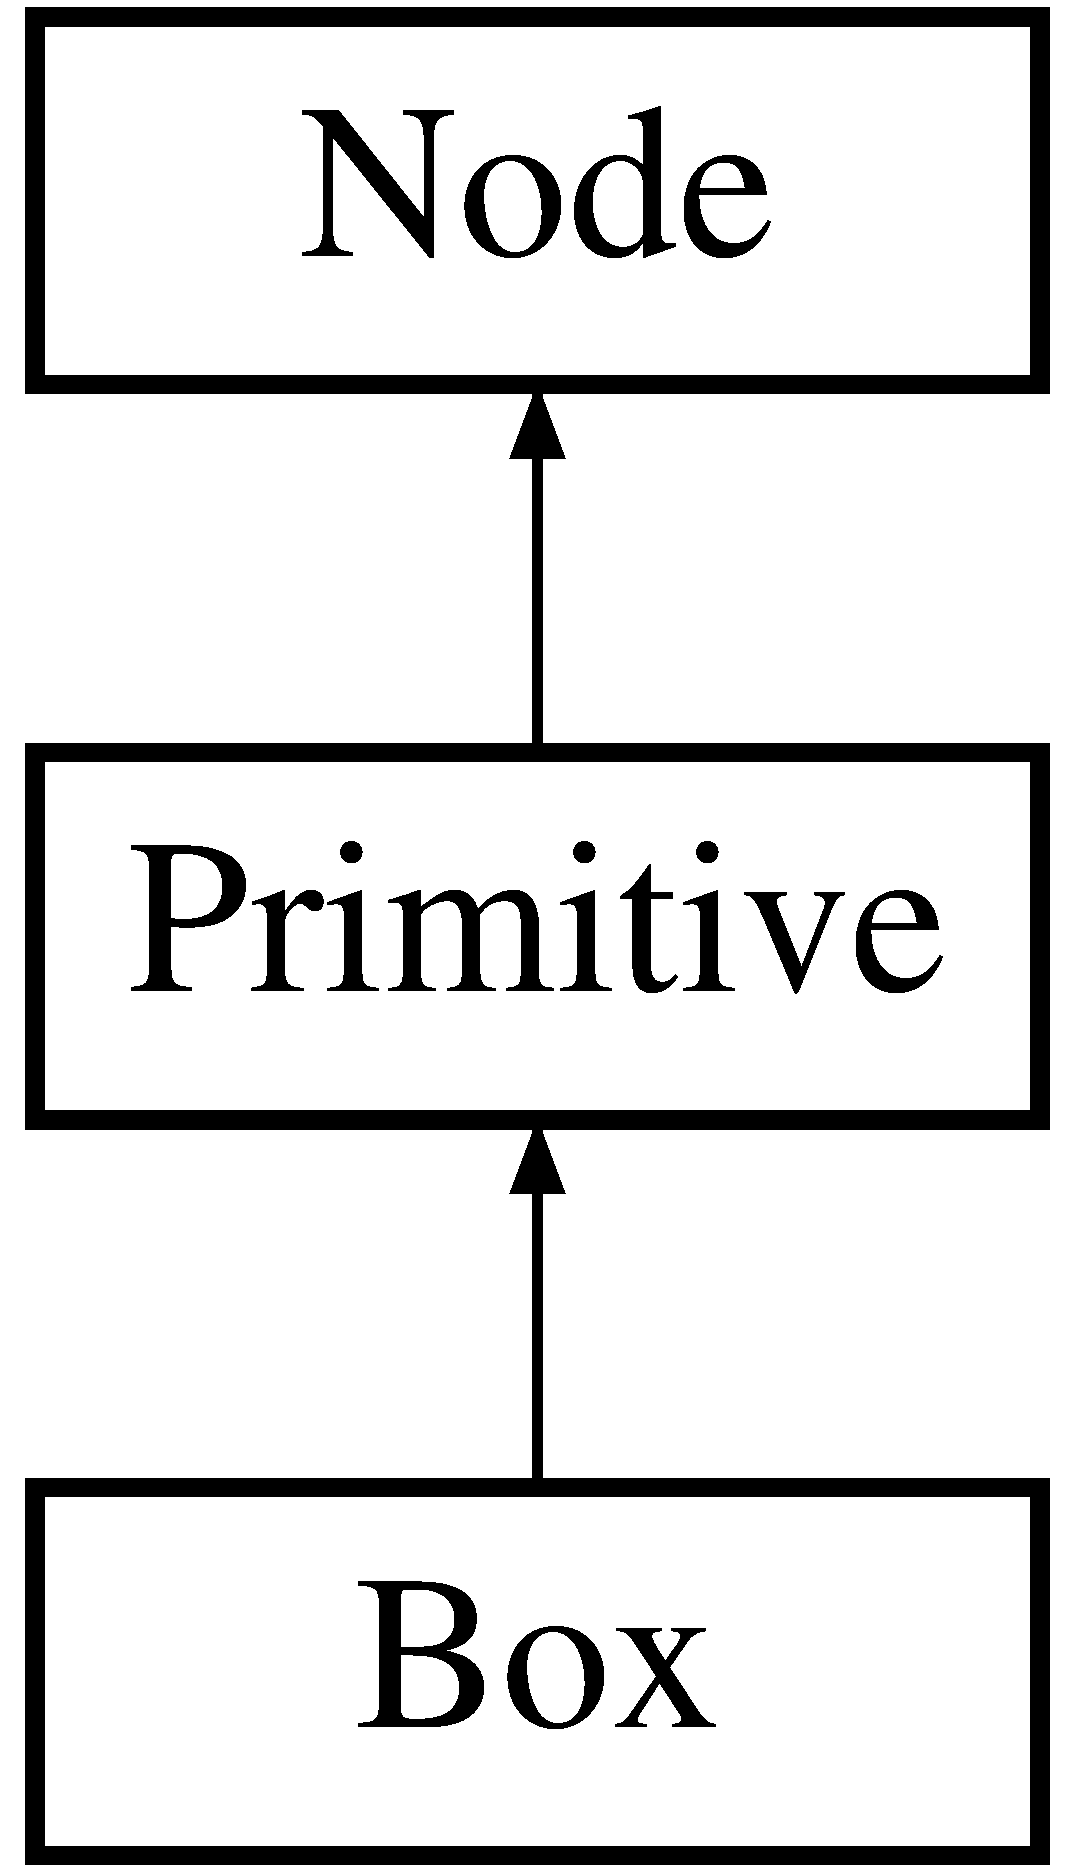
\includegraphics[height=3.000000cm]{class_box}
\end{center}
\end{figure}
\subsection*{\-Public \-Member \-Functions}
\begin{DoxyCompactItemize}
\item 
\hypertarget{class_box_aca78d7db44972bfa78d46b7bbc8796f6}{
\hyperlink{class_box_aca78d7db44972bfa78d46b7bbc8796f6}{\-Box} ()}
\label{class_box_aca78d7db44972bfa78d46b7bbc8796f6}

\begin{DoxyCompactList}\small\item\em \-Creates a generic box (empty). \end{DoxyCompactList}\item 
\hypertarget{class_box_ab4a2a18916c428de651b22cdf280bf3e}{
{\bfseries \-Box} (const \hyperlink{class_vector}{\-Vector} \&)}
\label{class_box_ab4a2a18916c428de651b22cdf280bf3e}

\item 
\hypertarget{class_box_a1f9d59659dc2304ed62088464f48c4da}{
{\bfseries \-Box} (const \hyperlink{class_vector}{\-Vector} \&, const \hyperlink{class_vector}{\-Vector} \&, const \hyperlink{class_vector}{\-Vector} \&, const \hyperlink{class_vector}{\-Vector} \&, int)}
\label{class_box_a1f9d59659dc2304ed62088464f48c4da}

\item 
\hypertarget{class_box_aa151dd75dfbe1632979853fe157322ea}{
{\bfseries \-Box} (const \hyperlink{class_vector}{\-Vector} \&, const double \&)}
\label{class_box_aa151dd75dfbe1632979853fe157322ea}

\item 
\hypertarget{class_box_a85ed08338073ace8d12833af0c861efb}{
{\bfseries \-Box} (\hyperlink{class_vector}{\-Vector} $\ast$, int)}
\label{class_box_a85ed08338073ace8d12833af0c861efb}

\item 
\hypertarget{class_box_a0a7c6f0b0405db01518bb3201b00c9a2}{
{\bfseries \-Box} (const \hyperlink{class_box}{\-Box} \&, const \hyperlink{class_box}{\-Box} \&)}
\label{class_box_a0a7c6f0b0405db01518bb3201b00c9a2}

\item 
\hypertarget{class_box_a6a5e09398e85d602a046b429062fb9c2}{
\hyperlink{class_box_a6a5e09398e85d602a046b429062fb9c2}{$\sim$\-Box} ()}
\label{class_box_a6a5e09398e85d602a046b429062fb9c2}

\begin{DoxyCompactList}\small\item\em \-Destroy a box, empty. \end{DoxyCompactList}\item 
\hypertarget{class_box_ad41f9a6efac5787613914b12e4c3d11d}{
\hyperlink{class_vector}{\-Vector} \& \hyperlink{class_box_ad41f9a6efac5787613914b12e4c3d11d}{operator\mbox{[}$\,$\mbox{]}} (int)}
\label{class_box_ad41f9a6efac5787613914b12e4c3d11d}

\begin{DoxyCompactList}\small\item\em \-Returns either end vertex of the box. \end{DoxyCompactList}\item 
\hypertarget{class_box_ae638073ba0eb5b6cb7a1f9de3b9a7bd8}{
\hyperlink{class_vector}{\-Vector} \hyperlink{class_box_ae638073ba0eb5b6cb7a1f9de3b9a7bd8}{operator\mbox{[}$\,$\mbox{]}} (int) const }
\label{class_box_ae638073ba0eb5b6cb7a1f9de3b9a7bd8}

\begin{DoxyCompactList}\small\item\em \-Overloaded. \end{DoxyCompactList}\item 
\hypertarget{class_box_a44e2805cb2a7acaaa3937522fae56d23}{
\hyperlink{class_vector}{\-Vector} \hyperlink{class_box_a44e2805cb2a7acaaa3937522fae56d23}{\-Center} () const }
\label{class_box_a44e2805cb2a7acaaa3937522fae56d23}

\begin{DoxyCompactList}\small\item\em \-Returns the center of the box. \end{DoxyCompactList}\item 
\hypertarget{class_box_a3e077400dd38d177c39bcc711788eed9}{
\hyperlink{class_vector}{\-Vector} \hyperlink{class_box_a3e077400dd38d177c39bcc711788eed9}{\-Diagonal} () const }
\label{class_box_a3e077400dd38d177c39bcc711788eed9}

\begin{DoxyCompactList}\small\item\em \-Returns the half diagonal of the box. \end{DoxyCompactList}\item 
\hypertarget{class_box_a44dd9300bf9713c9190c3a1e69ef5728}{
double \hyperlink{class_box_a44dd9300bf9713c9190c3a1e69ef5728}{\-Radius} () const }
\label{class_box_a44dd9300bf9713c9190c3a1e69ef5728}

\begin{DoxyCompactList}\small\item\em \-Returns the radius of the box, i.\-e. the length of the half diagonal of the box. \end{DoxyCompactList}\item 
\hypertarget{class_box_a35f5775304c754981b8a38d141737880}{
\hyperlink{class_vector}{\-Vector} \hyperlink{class_box_a35f5775304c754981b8a38d141737880}{\-Vertex} (int) const }
\label{class_box_a35f5775304c754981b8a38d141737880}

\begin{DoxyCompactList}\small\item\em \-Returns the k$^{\mbox{th}}$  vertex of the box. \end{DoxyCompactList}\item 
\hypertarget{class_box_a913a6b1487999917a85d87b49b3c1c52}{
double \hyperlink{class_box_a913a6b1487999917a85d87b49b3c1c52}{\-R} (const \hyperlink{class_vector}{\-Vector} \&) const }
\label{class_box_a913a6b1487999917a85d87b49b3c1c52}

\begin{DoxyCompactList}\small\item\em \-Computes the minimum distance between the box and a point in space. \end{DoxyCompactList}\item 
\hypertarget{class_box_a80db61cd35cae3122fe658ac079495ee}{
\hyperlink{class_vector}{\-Vector} \hyperlink{class_box_a80db61cd35cae3122fe658ac079495ee}{\-Normal} (const \hyperlink{class_vector}{\-Vector} \&) const }
\label{class_box_a80db61cd35cae3122fe658ac079495ee}

\begin{DoxyCompactList}\small\item\em \-Computes the normal vector between a point and a box. \end{DoxyCompactList}\item 
int \hyperlink{class_box_a6ac204afbbdc851645f33df16104292a}{\-Intersect} (const \hyperlink{class_ray}{\-Ray} \&, \hyperlink{class_intersection}{\-Intersection} \&)
\begin{DoxyCompactList}\small\item\em \-Intersecting function. \end{DoxyCompactList}\item 
int \hyperlink{class_box_a53e6a5db3bcc420700f88e6759da805d}{\-Intersect} (const \hyperlink{class_ray}{\-Ray} \&, \hyperlink{class_intersection}{\-Intersection} \&, \hyperlink{class_intersection}{\-Intersection} \&)
\begin{DoxyCompactList}\small\item\em \-Intersecting function. \end{DoxyCompactList}\item 
int \hyperlink{class_box_a13633b69e0fa7b8e6ca35c5d0fc65a8a}{\-Intersect} (const \hyperlink{class_ray}{\-Ray} \&, double \&, \hyperlink{class_vector}{\-Vector} \&) const 
\begin{DoxyCompactList}\small\item\em \-Intersecting function. \end{DoxyCompactList}\item 
\hypertarget{class_box_ac5702737ae3929edb195e49d48abe25d}{
int {\bfseries \-Intersect} (const \hyperlink{class_box}{\-Box} \&) const }
\label{class_box_ac5702737ae3929edb195e49d48abe25d}

\item 
int \hyperlink{class_box_abc15073158a80e02f4b1fb32b50e1eb6}{\-Inside} (const \hyperlink{class_box}{\-Box} \&) const 
\begin{DoxyCompactList}\small\item\em \-Containing function. \end{DoxyCompactList}\item 
int \hyperlink{class_box_aa3a80d26840216d02e1096e28333d65b}{\-Inside} (const \hyperlink{class_vector}{\-Vector} \&) const 
\begin{DoxyCompactList}\small\item\em \-Containing function. \end{DoxyCompactList}\item 
int \hyperlink{class_box_afb71788385a4f8ff91c6d8385972dde4}{\-P\-M\-C} (const \hyperlink{class_vector}{\-Vector} \&)
\begin{DoxyCompactList}\small\item\em \-Containing function. \end{DoxyCompactList}\item 
\hypertarget{class_box_ae6092debba95840365b79a02f60d245c}{
double \hyperlink{class_box_ae6092debba95840365b79a02f60d245c}{\-Volume} () const }
\label{class_box_ae6092debba95840365b79a02f60d245c}

\begin{DoxyCompactList}\small\item\em \-Compute the volume of a box. \end{DoxyCompactList}\item 
\hypertarget{class_box_a8e0a710afacb0bdeb3f751b40ab575b2}{
double \hyperlink{class_box_a8e0a710afacb0bdeb3f751b40ab575b2}{\-Area} () const }
\label{class_box_a8e0a710afacb0bdeb3f751b40ab575b2}

\begin{DoxyCompactList}\small\item\em \-Compute the surface area of a box. \end{DoxyCompactList}\item 
\hypertarget{class_box_a7bde7216a8ec3c840bdfd171f6c9b170}{
\hyperlink{class_vector}{\-Vector} {\bfseries get\-Position} ()}
\label{class_box_a7bde7216a8ec3c840bdfd171f6c9b170}

\end{DoxyCompactItemize}
\subsection*{\-Static \-Public \-Attributes}
\begin{DoxyCompactItemize}
\item 
static const double \hyperlink{class_box_ab038c94f04821a9ab0e0313819e5187c}{epsilon}
\end{DoxyCompactItemize}
\subsection*{\-Protected \-Attributes}
\begin{DoxyCompactItemize}
\item 
\hyperlink{class_vector}{\-Vector} \hyperlink{class_box_af9c25486a750badb5e746ba616e44bce}{a}
\item 
\hyperlink{class_vector}{\-Vector} \hyperlink{class_box_a9ba6812e3bc99ab5faf29f44550b57f5}{b}
\end{DoxyCompactItemize}


\subsection{\-Detailed \-Description}
\hyperlink{class_box}{\-Box} class. 

\hyperlink{class_box}{\-Box} is a primitive of the \-C\-S\-G 

\subsection{\-Member \-Function \-Documentation}
\hypertarget{class_box_abc15073158a80e02f4b1fb32b50e1eb6}{
\index{\-Box@{\-Box}!\-Inside@{\-Inside}}
\index{\-Inside@{\-Inside}!Box@{\-Box}}
\subsubsection[{\-Inside}]{\setlength{\rightskip}{0pt plus 5cm}int \-Box\-::\-Inside (
\begin{DoxyParamCaption}
\item[{const {\bf \-Box} \&}]{}
\end{DoxyParamCaption}
) const}}
\label{class_box_abc15073158a80e02f4b1fb32b50e1eb6}


\-Containing function. 

\-Checks if a box is inside the instance


\begin{DoxyParams}{\-Parameters}
{\em box} & \-: the box \\
\hline
\end{DoxyParams}
\hypertarget{class_box_aa3a80d26840216d02e1096e28333d65b}{
\index{\-Box@{\-Box}!\-Inside@{\-Inside}}
\index{\-Inside@{\-Inside}!Box@{\-Box}}
\subsubsection[{\-Inside}]{\setlength{\rightskip}{0pt plus 5cm}int \-Box\-::\-Inside (
\begin{DoxyParamCaption}
\item[{const {\bf \-Vector} \&}]{}
\end{DoxyParamCaption}
) const}}
\label{class_box_aa3a80d26840216d02e1096e28333d65b}


\-Containing function. 

\-Checks if a point is inside the instance


\begin{DoxyParams}{\-Parameters}
{\em u} & \-: the box \\
\hline
\end{DoxyParams}
\hypertarget{class_box_a6ac204afbbdc851645f33df16104292a}{
\index{\-Box@{\-Box}!\-Intersect@{\-Intersect}}
\index{\-Intersect@{\-Intersect}!Box@{\-Box}}
\subsubsection[{\-Intersect}]{\setlength{\rightskip}{0pt plus 5cm}int \-Box\-::\-Intersect (
\begin{DoxyParamCaption}
\item[{const {\bf \-Ray} \&}]{, }
\item[{{\bf \-Intersection} \&}]{}
\end{DoxyParamCaption}
)\hspace{0.3cm}{\ttfamily  \mbox{[}virtual\mbox{]}}}}
\label{class_box_a6ac204afbbdc851645f33df16104292a}


\-Intersecting function. 

\-Compute the intersection between a box and a ray


\begin{DoxyParams}{\-Parameters}
{\em ray} & \-: the ray \\
\hline
{\em inter1} & \-: the intersection \\
\hline
\end{DoxyParams}


\-Implements \hyperlink{class_node_ac0836475b7b0275dffe5ce89547f6852}{\-Node}.

\hypertarget{class_box_a53e6a5db3bcc420700f88e6759da805d}{
\index{\-Box@{\-Box}!\-Intersect@{\-Intersect}}
\index{\-Intersect@{\-Intersect}!Box@{\-Box}}
\subsubsection[{\-Intersect}]{\setlength{\rightskip}{0pt plus 5cm}int \-Box\-::\-Intersect (
\begin{DoxyParamCaption}
\item[{const {\bf \-Ray} \&}]{, }
\item[{{\bf \-Intersection} \&}]{, }
\item[{{\bf \-Intersection} \&}]{}
\end{DoxyParamCaption}
)\hspace{0.3cm}{\ttfamily  \mbox{[}virtual\mbox{]}}}}
\label{class_box_a53e6a5db3bcc420700f88e6759da805d}


\-Intersecting function. 

\-Compute the intersections between a box and a ray


\begin{DoxyParams}{\-Parameters}
{\em ray} & \-: the ray \\
\hline
{\em inter1} & \-: the first intersection \\
\hline
{\em inter2} & \-: the second intersection \\
\hline
\end{DoxyParams}


\-Implements \hyperlink{class_node_a8f308647523fba2603248b83149855a5}{\-Node}.

\hypertarget{class_box_a13633b69e0fa7b8e6ca35c5d0fc65a8a}{
\index{\-Box@{\-Box}!\-Intersect@{\-Intersect}}
\index{\-Intersect@{\-Intersect}!Box@{\-Box}}
\subsubsection[{\-Intersect}]{\setlength{\rightskip}{0pt plus 5cm}int \-Box\-::\-Intersect (
\begin{DoxyParamCaption}
\item[{const {\bf \-Ray} \&}]{, }
\item[{double \&}]{, }
\item[{{\bf \-Vector} \&}]{}
\end{DoxyParamCaption}
) const}}
\label{class_box_a13633b69e0fa7b8e6ca35c5d0fc65a8a}


\-Intersecting function. 

\-Compute the first positive intersection between an axis aligned box and a ray


\begin{DoxyParams}{\-Parameters}
{\em ray} & \-: the ray \\
\hline
{\em t} & \-: the first intersection \\
\hline
{\em n} & \-: the normal at intersection point \\
\hline
\end{DoxyParams}
\hypertarget{class_box_afb71788385a4f8ff91c6d8385972dde4}{
\index{\-Box@{\-Box}!\-P\-M\-C@{\-P\-M\-C}}
\index{\-P\-M\-C@{\-P\-M\-C}!Box@{\-Box}}
\subsubsection[{\-P\-M\-C}]{\setlength{\rightskip}{0pt plus 5cm}int \-Box\-::\-P\-M\-C (
\begin{DoxyParamCaption}
\item[{const {\bf \-Vector} \&}]{}
\end{DoxyParamCaption}
)\hspace{0.3cm}{\ttfamily  \mbox{[}virtual\mbox{]}}}}
\label{class_box_afb71788385a4f8ff91c6d8385972dde4}


\-Containing function. 

\-Checks if a point is inside the instance


\begin{DoxyParams}{\-Parameters}
{\em u} & \-: the point \\
\hline
\end{DoxyParams}


\-Implements \hyperlink{class_node_aeecdf01a88be40840b65eb34cecc7a3c}{\-Node}.



\subsection{\-Member \-Data \-Documentation}
\hypertarget{class_box_af9c25486a750badb5e746ba616e44bce}{
\index{\-Box@{\-Box}!a@{a}}
\index{a@{a}!Box@{\-Box}}
\subsubsection[{a}]{\setlength{\rightskip}{0pt plus 5cm}{\bf \-Vector} {\bf \-Box\-::a}\hspace{0.3cm}{\ttfamily  \mbox{[}protected\mbox{]}}}}
\label{class_box_af9c25486a750badb5e746ba616e44bce}
\hyperlink{class_box}{\-Box} bottom left point \hypertarget{class_box_a9ba6812e3bc99ab5faf29f44550b57f5}{
\index{\-Box@{\-Box}!b@{b}}
\index{b@{b}!Box@{\-Box}}
\subsubsection[{b}]{\setlength{\rightskip}{0pt plus 5cm}{\bf \-Vector} {\bf \-Box\-::b}\hspace{0.3cm}{\ttfamily  \mbox{[}protected\mbox{]}}}}
\label{class_box_a9ba6812e3bc99ab5faf29f44550b57f5}
\hyperlink{class_box}{\-Box} upper right point \hypertarget{class_box_ab038c94f04821a9ab0e0313819e5187c}{
\index{\-Box@{\-Box}!epsilon@{epsilon}}
\index{epsilon@{epsilon}!Box@{\-Box}}
\subsubsection[{epsilon}]{\setlength{\rightskip}{0pt plus 5cm}const double {\bf \-Box\-::epsilon}\hspace{0.3cm}{\ttfamily  \mbox{[}static\mbox{]}}}}
\label{class_box_ab038c94f04821a9ab0e0313819e5187c}
\-Epsilon value used to check intersections and some round off errors 

\-The documentation for this class was generated from the following file\-:\begin{DoxyCompactItemize}
\item 
headers/\hyperlink{box_8h}{box.\-h}\end{DoxyCompactItemize}

\hypertarget{class_cylinder}{
\section{\-Cylinder \-Class \-Reference}
\label{class_cylinder}\index{\-Cylinder@{\-Cylinder}}
}


\hyperlink{class_cylinder}{\-Cylinder} class.  




{\ttfamily \#include $<$cylinder.\-h$>$}

\-Inheritance diagram for \-Cylinder\-:\begin{figure}[H]
\begin{center}
\leavevmode
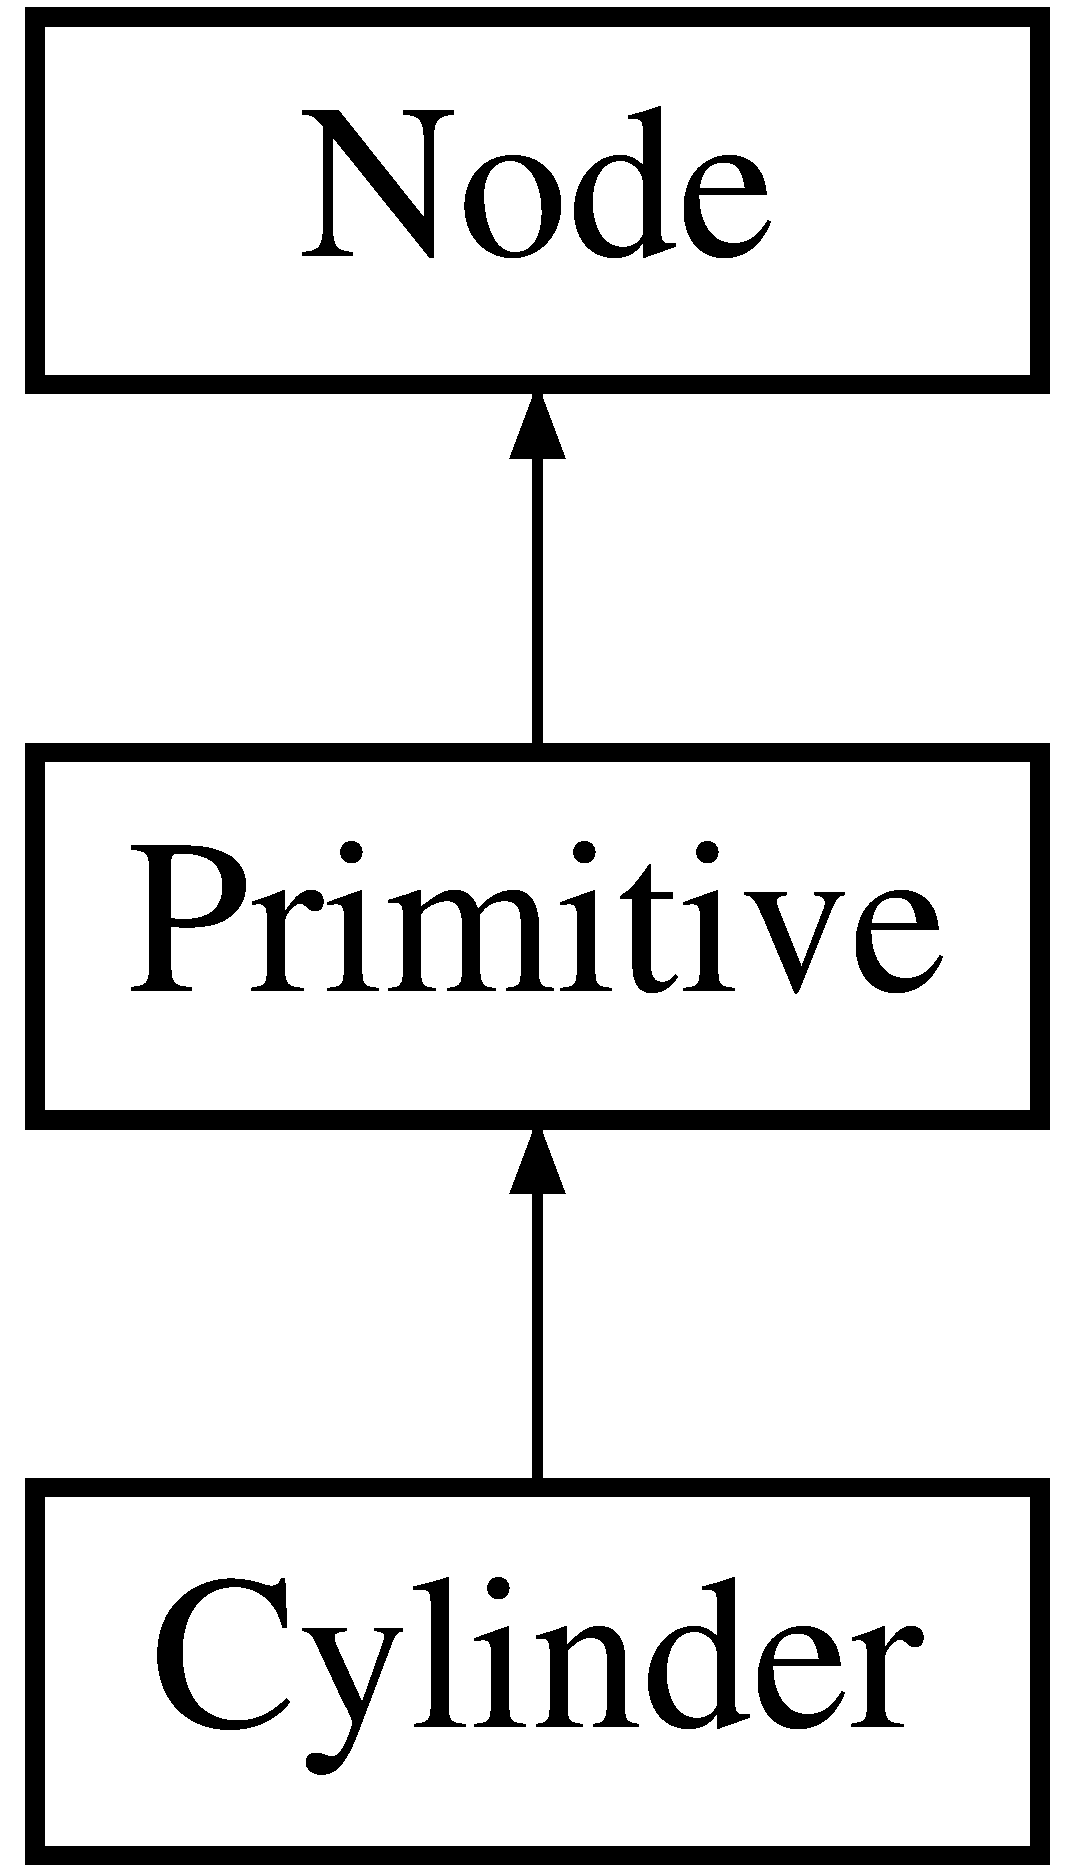
\includegraphics[height=3.000000cm]{class_cylinder}
\end{center}
\end{figure}
\subsection*{\-Public \-Member \-Functions}
\begin{DoxyCompactItemize}
\item 
\hypertarget{class_cylinder_aac916600a494275d514aa7ca14d1e61a}{
{\bfseries \-Cylinder} (const double \&, const \hyperlink{class_vector}{\-Vector} \&, const double, const \hyperlink{class_vector}{\-Vector} \&, const \hyperlink{class_vector}{\-Vector} \&, int)}
\label{class_cylinder_aac916600a494275d514aa7ca14d1e61a}

\item 
int \hyperlink{class_cylinder_ac0fefa4e21c59f64bd1b52d46ffc660f}{\-Intersect} (const \hyperlink{class_ray}{\-Ray} \&, \hyperlink{class_intersection}{\-Intersection} \&)
\begin{DoxyCompactList}\small\item\em \-Intersecting function. \end{DoxyCompactList}\item 
int \hyperlink{class_cylinder_ad5f756db8354800d0a95862f6de2a5fe}{\-Intersect} (const \hyperlink{class_ray}{\-Ray} \&, \hyperlink{class_intersection}{\-Intersection} \&, \hyperlink{class_intersection}{\-Intersection} \&)
\begin{DoxyCompactList}\small\item\em \-Intersecting function. \end{DoxyCompactList}\item 
int \hyperlink{class_cylinder_a54d8f47f574488e583868fbd5dfd9abf}{\-P\-M\-C} (const \hyperlink{class_vector}{\-Vector} \&)
\begin{DoxyCompactList}\small\item\em \-P\-M\-C function. \end{DoxyCompactList}\item 
\hyperlink{class_vector}{\-Vector} \hyperlink{class_cylinder_aaec0c6f325302a116df1d210791b575c}{get\-Position} ()
\begin{DoxyCompactList}\small\item\em \-Get position function. \end{DoxyCompactList}\end{DoxyCompactItemize}
\subsection*{\-Protected \-Attributes}
\begin{DoxyCompactItemize}
\item 
double \hyperlink{class_cylinder_a8a825799285bcf60b49b8aef0459b498}{radius}
\item 
double \hyperlink{class_cylinder_a211cebc37f1025850cdacffe1badb578}{height}
\item 
\hyperlink{class_vector}{\-Vector} \hyperlink{class_cylinder_ad6d4d4070807f4680a250ec1227fc482}{bottom}
\end{DoxyCompactItemize}


\subsection{\-Detailed \-Description}
\hyperlink{class_cylinder}{\-Cylinder} class. 

\hyperlink{class_cylinder}{\-Cylinder} is a primitive of the \-C\-S\-G 

\subsection{\-Member \-Function \-Documentation}
\hypertarget{class_cylinder_aaec0c6f325302a116df1d210791b575c}{
\index{\-Cylinder@{\-Cylinder}!get\-Position@{get\-Position}}
\index{get\-Position@{get\-Position}!Cylinder@{\-Cylinder}}
\subsubsection[{get\-Position}]{\setlength{\rightskip}{0pt plus 5cm}{\bf \-Vector} \-Cylinder\-::get\-Position (
\begin{DoxyParamCaption}
{}
\end{DoxyParamCaption}
)\hspace{0.3cm}{\ttfamily  \mbox{[}virtual\mbox{]}}}}
\label{class_cylinder_aaec0c6f325302a116df1d210791b575c}


\-Get position function. 

\-Compute the cylinder position 

\-Implements \hyperlink{class_node}{\-Node}.

\hypertarget{class_cylinder_ac0fefa4e21c59f64bd1b52d46ffc660f}{
\index{\-Cylinder@{\-Cylinder}!\-Intersect@{\-Intersect}}
\index{\-Intersect@{\-Intersect}!Cylinder@{\-Cylinder}}
\subsubsection[{\-Intersect}]{\setlength{\rightskip}{0pt plus 5cm}int \-Cylinder\-::\-Intersect (
\begin{DoxyParamCaption}
\item[{const {\bf \-Ray} \&}]{, }
\item[{{\bf \-Intersection} \&}]{}
\end{DoxyParamCaption}
)\hspace{0.3cm}{\ttfamily  \mbox{[}virtual\mbox{]}}}}
\label{class_cylinder_ac0fefa4e21c59f64bd1b52d46ffc660f}


\-Intersecting function. 

\-Compute the intersection between a node and a ray


\begin{DoxyParams}{\-Parameters}
{\em ray} & \-: the ray \\
\hline
{\em t} & \-: the intersection \\
\hline
\end{DoxyParams}


\-Implements \hyperlink{class_node_ac0836475b7b0275dffe5ce89547f6852}{\-Node}.

\hypertarget{class_cylinder_ad5f756db8354800d0a95862f6de2a5fe}{
\index{\-Cylinder@{\-Cylinder}!\-Intersect@{\-Intersect}}
\index{\-Intersect@{\-Intersect}!Cylinder@{\-Cylinder}}
\subsubsection[{\-Intersect}]{\setlength{\rightskip}{0pt plus 5cm}int \-Cylinder\-::\-Intersect (
\begin{DoxyParamCaption}
\item[{const {\bf \-Ray} \&}]{, }
\item[{{\bf \-Intersection} \&}]{, }
\item[{{\bf \-Intersection} \&}]{}
\end{DoxyParamCaption}
)\hspace{0.3cm}{\ttfamily  \mbox{[}virtual\mbox{]}}}}
\label{class_cylinder_ad5f756db8354800d0a95862f6de2a5fe}


\-Intersecting function. 

\-Compute the intersections between a cylinder and a ray


\begin{DoxyParams}{\-Parameters}
{\em ray} & \-: the ray \\
\hline
{\em inter1} & \-: the first intersection \\
\hline
{\em inter2} & \-: the second intersection \\
\hline
\end{DoxyParams}


\-Implements \hyperlink{class_node_a8f308647523fba2603248b83149855a5}{\-Node}.

\hypertarget{class_cylinder_a54d8f47f574488e583868fbd5dfd9abf}{
\index{\-Cylinder@{\-Cylinder}!\-P\-M\-C@{\-P\-M\-C}}
\index{\-P\-M\-C@{\-P\-M\-C}!Cylinder@{\-Cylinder}}
\subsubsection[{\-P\-M\-C}]{\setlength{\rightskip}{0pt plus 5cm}int \-Cylinder\-::\-P\-M\-C (
\begin{DoxyParamCaption}
\item[{const {\bf \-Vector} \&}]{}
\end{DoxyParamCaption}
)\hspace{0.3cm}{\ttfamily  \mbox{[}virtual\mbox{]}}}}
\label{class_cylinder_a54d8f47f574488e583868fbd5dfd9abf}


\-P\-M\-C function. 

\-Compute if the point is in the cylinder


\begin{DoxyParams}{\-Parameters}
{\em point} & \-: the point \\
\hline
\end{DoxyParams}


\-Implements \hyperlink{class_node_aeecdf01a88be40840b65eb34cecc7a3c}{\-Node}.



\subsection{\-Member \-Data \-Documentation}
\hypertarget{class_cylinder_ad6d4d4070807f4680a250ec1227fc482}{
\index{\-Cylinder@{\-Cylinder}!bottom@{bottom}}
\index{bottom@{bottom}!Cylinder@{\-Cylinder}}
\subsubsection[{bottom}]{\setlength{\rightskip}{0pt plus 5cm}{\bf \-Vector} {\bf \-Cylinder\-::bottom}\hspace{0.3cm}{\ttfamily  \mbox{[}protected\mbox{]}}}}
\label{class_cylinder_ad6d4d4070807f4680a250ec1227fc482}
\hyperlink{class_cylinder}{\-Cylinder} bottom center \hypertarget{class_cylinder_a211cebc37f1025850cdacffe1badb578}{
\index{\-Cylinder@{\-Cylinder}!height@{height}}
\index{height@{height}!Cylinder@{\-Cylinder}}
\subsubsection[{height}]{\setlength{\rightskip}{0pt plus 5cm}double {\bf \-Cylinder\-::height}\hspace{0.3cm}{\ttfamily  \mbox{[}protected\mbox{]}}}}
\label{class_cylinder_a211cebc37f1025850cdacffe1badb578}
\hyperlink{class_cylinder}{\-Cylinder} upper lenght \hypertarget{class_cylinder_a8a825799285bcf60b49b8aef0459b498}{
\index{\-Cylinder@{\-Cylinder}!radius@{radius}}
\index{radius@{radius}!Cylinder@{\-Cylinder}}
\subsubsection[{radius}]{\setlength{\rightskip}{0pt plus 5cm}double {\bf \-Cylinder\-::radius}\hspace{0.3cm}{\ttfamily  \mbox{[}protected\mbox{]}}}}
\label{class_cylinder_a8a825799285bcf60b49b8aef0459b498}
\hyperlink{class_cylinder}{\-Cylinder} radius 

\-The documentation for this class was generated from the following file\-:\begin{DoxyCompactItemize}
\item 
headers/\hyperlink{cylinder_8h}{cylinder.\-h}\end{DoxyCompactItemize}

\hypertarget{class_diff}{
\section{\-Diff \-Class \-Reference}
\label{class_diff}\index{\-Diff@{\-Diff}}
}


\hyperlink{class_diff}{\-Diff} class.  




{\ttfamily \#include $<$diff.\-h$>$}

\-Inheritance diagram for \-Diff\-:\begin{figure}[H]
\begin{center}
\leavevmode
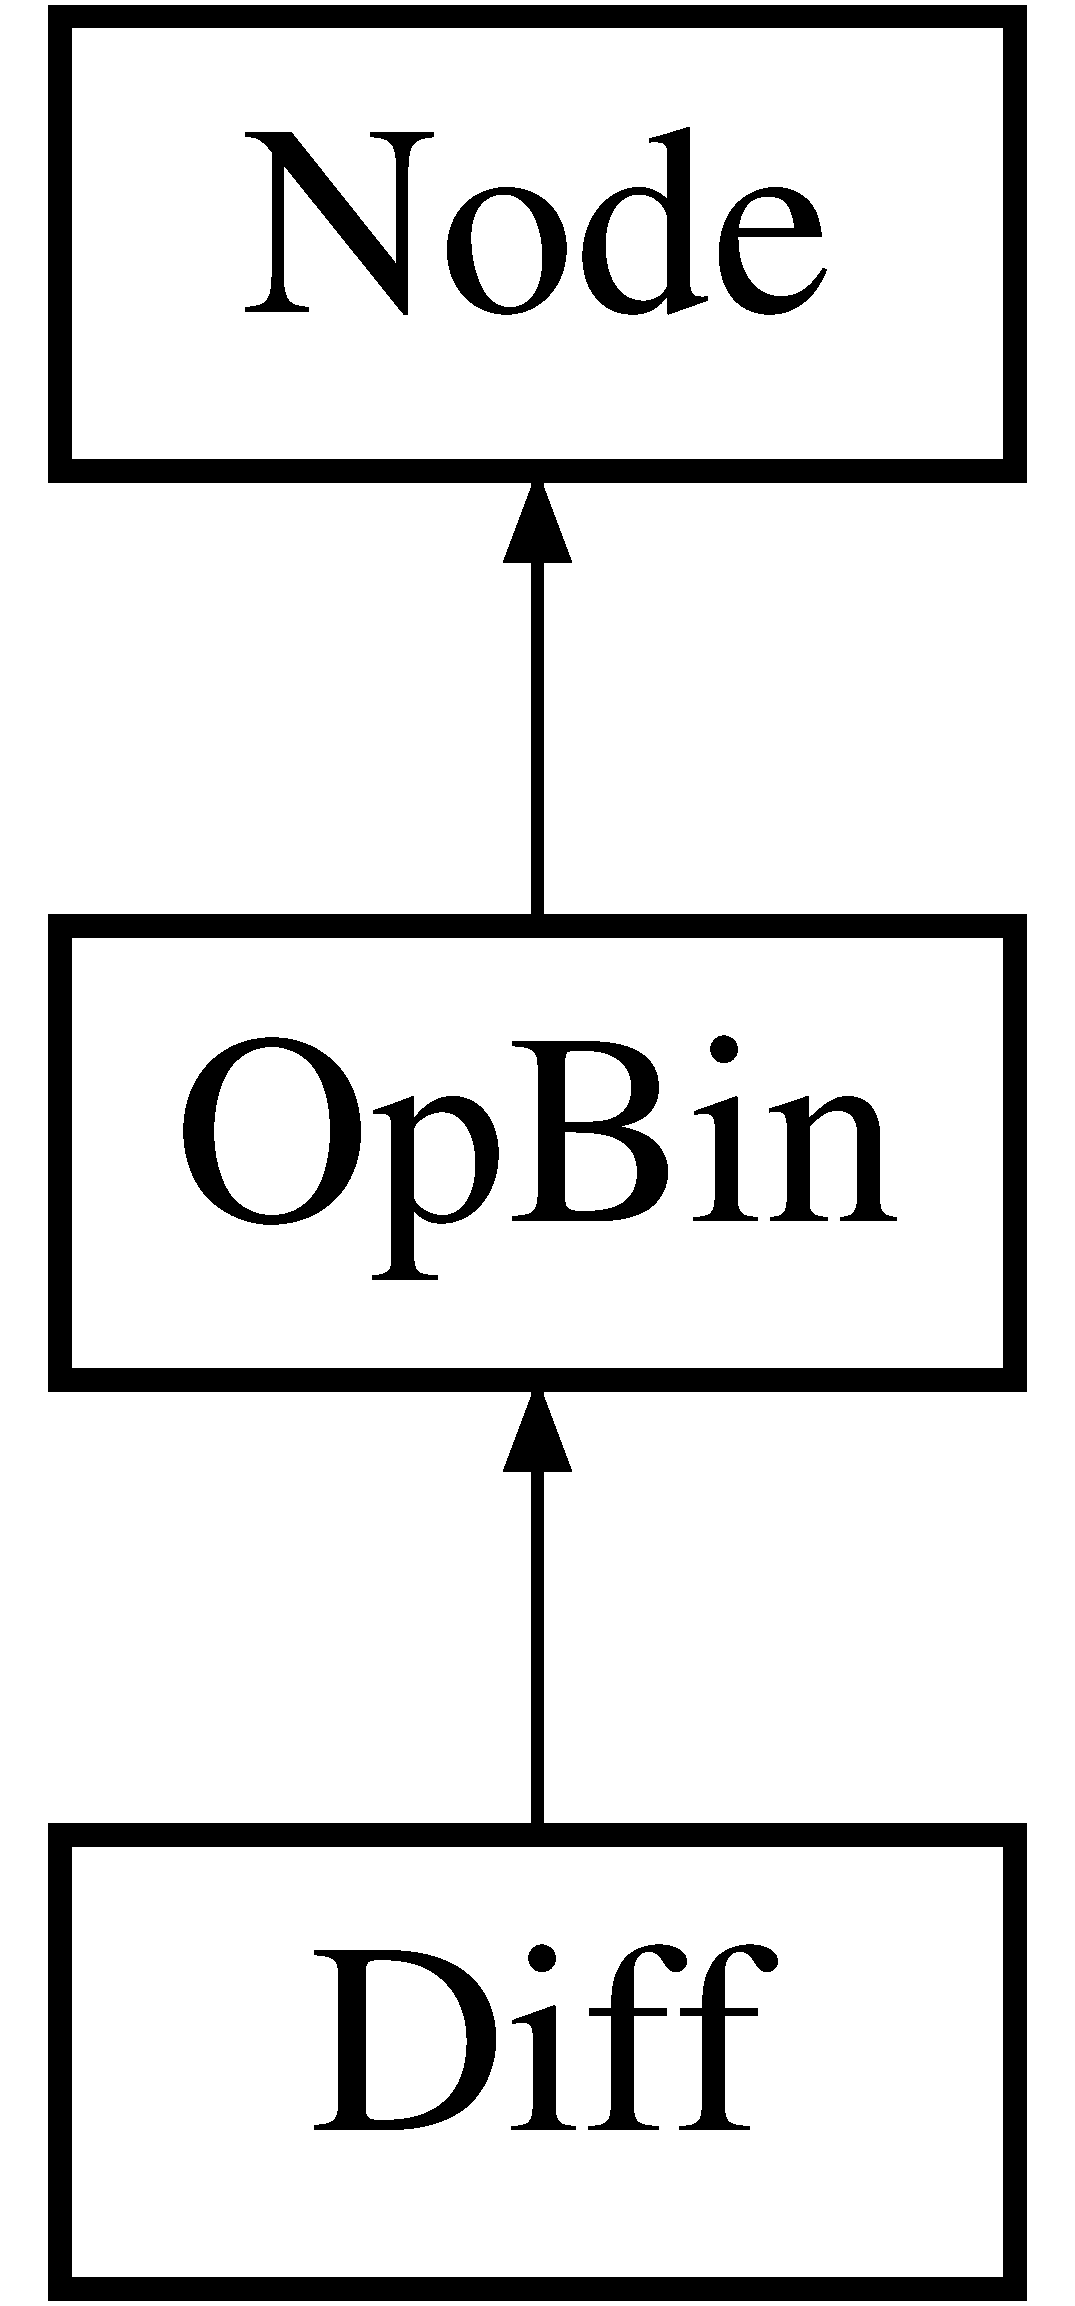
\includegraphics[height=3.000000cm]{class_diff}
\end{center}
\end{figure}
\subsection*{\-Public \-Member \-Functions}
\begin{DoxyCompactItemize}
\item 
\hypertarget{class_diff_a97d13870f4c698c6242937f91092330e}{
{\bfseries \-Diff} (\hyperlink{class_node}{\-Node} $\ast$, \hyperlink{class_node}{\-Node} $\ast$)}
\label{class_diff_a97d13870f4c698c6242937f91092330e}

\item 
int \hyperlink{class_diff_a9d9ee35accad3efbed3aba5fc9da022c}{\-Intersect} (const \hyperlink{class_ray}{\-Ray} \&, \hyperlink{class_intersection}{\-Intersection} \&)
\begin{DoxyCompactList}\small\item\em \-Intersecting function. \end{DoxyCompactList}\item 
int \hyperlink{class_diff_ad2e06f30b3998b3c9592821e9a037697}{\-Intersect} (const \hyperlink{class_ray}{\-Ray} \&, \hyperlink{class_intersection}{\-Intersection} \&, \hyperlink{class_intersection}{\-Intersection} \&)
\begin{DoxyCompactList}\small\item\em \-Intersecting function. \end{DoxyCompactList}\item 
int \hyperlink{class_diff_a9569764d64e3cc072c554ceffad7934a}{\-P\-M\-C} (const \hyperlink{class_vector}{\-Vector} \&)
\begin{DoxyCompactList}\small\item\em \-Containing function. \end{DoxyCompactList}\item 
\hypertarget{class_diff_a3c7c9dfc158002c877a4ef0aeac30900}{
\hyperlink{class_vector}{\-Vector} {\bfseries get\-Emission} ()}
\label{class_diff_a3c7c9dfc158002c877a4ef0aeac30900}

\item 
\hypertarget{class_diff_afb4a403e4cbc49710fb7b6f570c3fe39}{
\hyperlink{class_vector}{\-Vector} {\bfseries get\-Color} ()}
\label{class_diff_afb4a403e4cbc49710fb7b6f570c3fe39}

\item 
\hypertarget{class_diff_a8c962ee4f6a0df72e7a69322de3210b8}{
\hyperlink{class_vector}{\-Vector} {\bfseries get\-Position} ()}
\label{class_diff_a8c962ee4f6a0df72e7a69322de3210b8}

\item 
\hypertarget{class_diff_ad9c0799bfde75340e584a1ea20d7f564}{
int {\bfseries get\-Refl} ()}
\label{class_diff_ad9c0799bfde75340e584a1ea20d7f564}

\item 
\hypertarget{class_diff_a55bd9230b7be32d4e9a1e20a5ff5df10}{
double {\bfseries get\-F} ()}
\label{class_diff_a55bd9230b7be32d4e9a1e20a5ff5df10}

\end{DoxyCompactItemize}


\subsection{\-Detailed \-Description}
\hyperlink{class_diff}{\-Diff} class. 

\hyperlink{class_diff}{\-Diff} is a binary operand of the \-C\-S\-G 

\subsection{\-Member \-Function \-Documentation}
\hypertarget{class_diff_a9d9ee35accad3efbed3aba5fc9da022c}{
\index{\-Diff@{\-Diff}!\-Intersect@{\-Intersect}}
\index{\-Intersect@{\-Intersect}!Diff@{\-Diff}}
\subsubsection[{\-Intersect}]{\setlength{\rightskip}{0pt plus 5cm}int \-Diff\-::\-Intersect (
\begin{DoxyParamCaption}
\item[{const {\bf \-Ray} \&}]{, }
\item[{{\bf \-Intersection} \&}]{}
\end{DoxyParamCaption}
)\hspace{0.3cm}{\ttfamily  \mbox{[}virtual\mbox{]}}}}
\label{class_diff_a9d9ee35accad3efbed3aba5fc9da022c}


\-Intersecting function. 

\-Compute the intersection between a difference and a ray


\begin{DoxyParams}{\-Parameters}
{\em ray} & \-: the ray \\
\hline
{\em t} & \-: the intersection \\
\hline
\end{DoxyParams}


\-Implements \hyperlink{class_node_ac0836475b7b0275dffe5ce89547f6852}{\-Node}.

\hypertarget{class_diff_ad2e06f30b3998b3c9592821e9a037697}{
\index{\-Diff@{\-Diff}!\-Intersect@{\-Intersect}}
\index{\-Intersect@{\-Intersect}!Diff@{\-Diff}}
\subsubsection[{\-Intersect}]{\setlength{\rightskip}{0pt plus 5cm}int \-Diff\-::\-Intersect (
\begin{DoxyParamCaption}
\item[{const {\bf \-Ray} \&}]{, }
\item[{{\bf \-Intersection} \&}]{, }
\item[{{\bf \-Intersection} \&}]{}
\end{DoxyParamCaption}
)\hspace{0.3cm}{\ttfamily  \mbox{[}virtual\mbox{]}}}}
\label{class_diff_ad2e06f30b3998b3c9592821e9a037697}


\-Intersecting function. 

\-Compute the intersections between a difference and a ray


\begin{DoxyParams}{\-Parameters}
{\em ray} & \-: the ray \\
\hline
{\em t1} & \-: the first intersection \\
\hline
{\em t2} & \-: the second intersection \\
\hline
\end{DoxyParams}


\-Implements \hyperlink{class_node_a8f308647523fba2603248b83149855a5}{\-Node}.

\hypertarget{class_diff_a9569764d64e3cc072c554ceffad7934a}{
\index{\-Diff@{\-Diff}!\-P\-M\-C@{\-P\-M\-C}}
\index{\-P\-M\-C@{\-P\-M\-C}!Diff@{\-Diff}}
\subsubsection[{\-P\-M\-C}]{\setlength{\rightskip}{0pt plus 5cm}int \-Diff\-::\-P\-M\-C (
\begin{DoxyParamCaption}
\item[{const {\bf \-Vector} \&}]{}
\end{DoxyParamCaption}
)\hspace{0.3cm}{\ttfamily  \mbox{[}virtual\mbox{]}}}}
\label{class_diff_a9569764d64e3cc072c554ceffad7934a}


\-Containing function. 

\-Checks if a point is inside the instance


\begin{DoxyParams}{\-Parameters}
{\em u} & \-: the point \\
\hline
\end{DoxyParams}


\-Implements \hyperlink{class_node_aeecdf01a88be40840b65eb34cecc7a3c}{\-Node}.



\-The documentation for this class was generated from the following file\-:\begin{DoxyCompactItemize}
\item 
headers/\hyperlink{diff_8h}{diff.\-h}\end{DoxyCompactItemize}

\hypertarget{class_inter}{
\section{\-Inter \-Class \-Reference}
\label{class_inter}\index{\-Inter@{\-Inter}}
}


\hyperlink{class_inter}{\-Inter} class.  




{\ttfamily \#include $<$inter.\-h$>$}

\-Inheritance diagram for \-Inter\-:\begin{figure}[H]
\begin{center}
\leavevmode
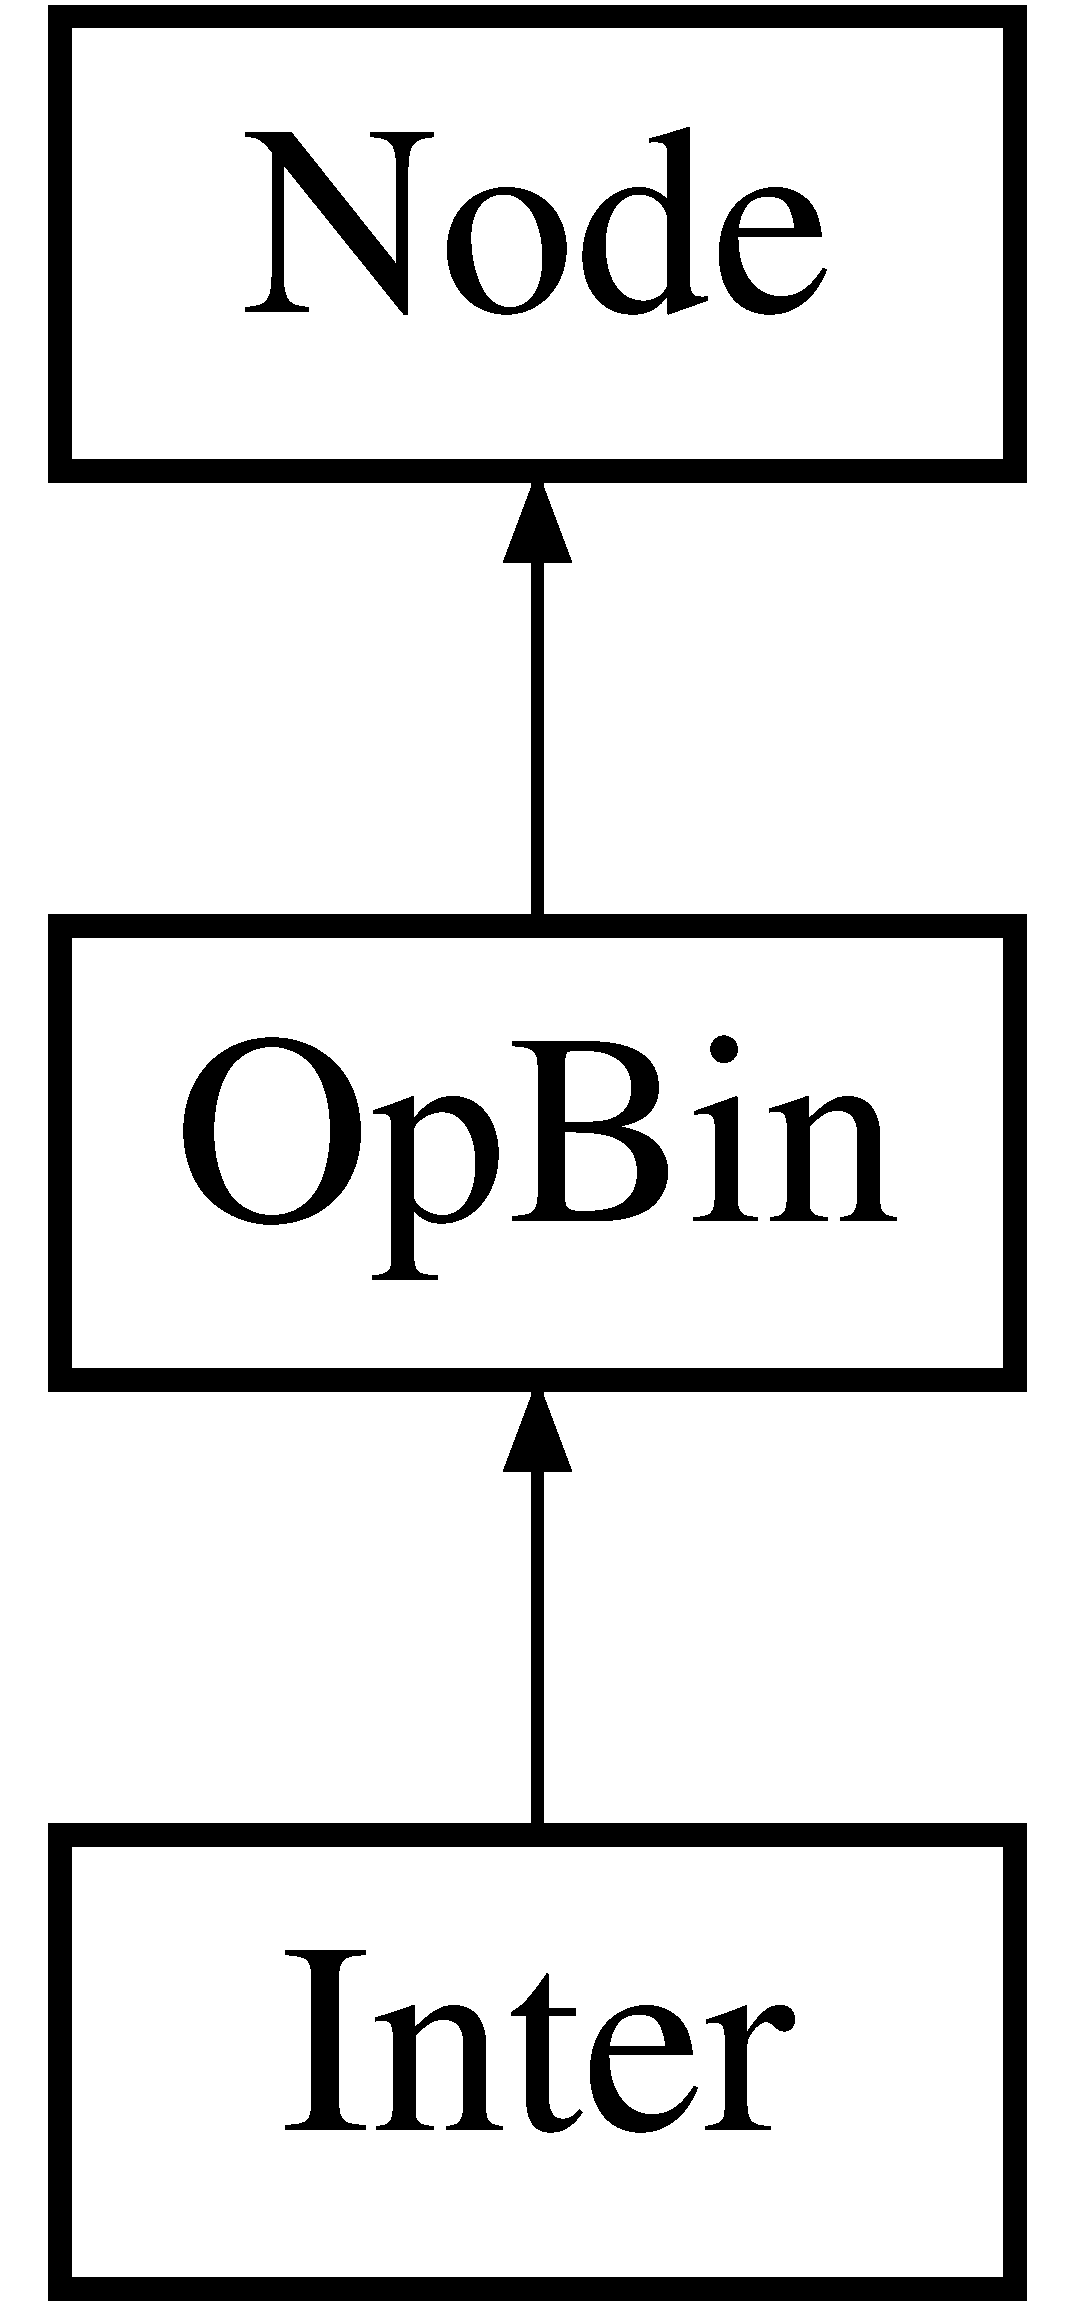
\includegraphics[height=3.000000cm]{class_inter}
\end{center}
\end{figure}
\subsection*{\-Public \-Member \-Functions}
\begin{DoxyCompactItemize}
\item 
\hypertarget{class_inter_aac4a41fc06f70c3daac8e38919cc9b79}{
{\bfseries \-Inter} (\hyperlink{class_node}{\-Node} $\ast$, \hyperlink{class_node}{\-Node} $\ast$)}
\label{class_inter_aac4a41fc06f70c3daac8e38919cc9b79}

\item 
int \hyperlink{class_inter_a8b67290ace7c86e6cba66b5571466204}{\-Intersect} (const \hyperlink{class_ray}{\-Ray} \&, \hyperlink{class_intersection}{\-Intersection} \&)
\begin{DoxyCompactList}\small\item\em \-Intersecting function. \end{DoxyCompactList}\item 
int \hyperlink{class_inter_a50b2aa819ddbd2c53d26e8e7342312da}{\-Intersect} (const \hyperlink{class_ray}{\-Ray} \&, \hyperlink{class_intersection}{\-Intersection} \&, \hyperlink{class_intersection}{\-Intersection} \&)
\begin{DoxyCompactList}\small\item\em \-Intersecting function. \end{DoxyCompactList}\item 
int \hyperlink{class_inter_a62fb756b8848c042f6ea48bbe204f4a6}{\-P\-M\-C} (const \hyperlink{class_vector}{\-Vector} \&)
\begin{DoxyCompactList}\small\item\em \-Containing function. \end{DoxyCompactList}\item 
\hypertarget{class_inter_a858d782251352e10594425ccff10b162}{
\hyperlink{class_vector}{\-Vector} {\bfseries get\-Emission} ()}
\label{class_inter_a858d782251352e10594425ccff10b162}

\item 
\hypertarget{class_inter_a9fafa04883ee457fd41e4a5cb0461470}{
\hyperlink{class_vector}{\-Vector} {\bfseries get\-Color} ()}
\label{class_inter_a9fafa04883ee457fd41e4a5cb0461470}

\item 
\hypertarget{class_inter_a2a1d193dacdbae9b7393fbdf3592c434}{
\hyperlink{class_vector}{\-Vector} {\bfseries get\-Position} ()}
\label{class_inter_a2a1d193dacdbae9b7393fbdf3592c434}

\item 
\hypertarget{class_inter_a6fe2fa17f2c74536482f8b24eee5cea4}{
int {\bfseries get\-Refl} ()}
\label{class_inter_a6fe2fa17f2c74536482f8b24eee5cea4}

\item 
\hypertarget{class_inter_affe69e09e6b0f4455699a23a93688cf4}{
double {\bfseries get\-F} ()}
\label{class_inter_affe69e09e6b0f4455699a23a93688cf4}

\end{DoxyCompactItemize}


\subsection{\-Detailed \-Description}
\hyperlink{class_inter}{\-Inter} class. 

\hyperlink{class_inter}{\-Inter} is a binary operand of the \-C\-S\-G 

\subsection{\-Member \-Function \-Documentation}
\hypertarget{class_inter_a8b67290ace7c86e6cba66b5571466204}{
\index{\-Inter@{\-Inter}!\-Intersect@{\-Intersect}}
\index{\-Intersect@{\-Intersect}!Inter@{\-Inter}}
\subsubsection[{\-Intersect}]{\setlength{\rightskip}{0pt plus 5cm}int \-Inter\-::\-Intersect (
\begin{DoxyParamCaption}
\item[{const {\bf \-Ray} \&}]{, }
\item[{{\bf \-Intersection} \&}]{}
\end{DoxyParamCaption}
)\hspace{0.3cm}{\ttfamily  \mbox{[}virtual\mbox{]}}}}
\label{class_inter_a8b67290ace7c86e6cba66b5571466204}


\-Intersecting function. 

\-Compute the intersection between a intersection and a ray


\begin{DoxyParams}{\-Parameters}
{\em ray} & \-: the ray \\
\hline
{\em t} & \-: the intersection \\
\hline
\end{DoxyParams}


\-Implements \hyperlink{class_node_ac0836475b7b0275dffe5ce89547f6852}{\-Node}.

\hypertarget{class_inter_a50b2aa819ddbd2c53d26e8e7342312da}{
\index{\-Inter@{\-Inter}!\-Intersect@{\-Intersect}}
\index{\-Intersect@{\-Intersect}!Inter@{\-Inter}}
\subsubsection[{\-Intersect}]{\setlength{\rightskip}{0pt plus 5cm}int \-Inter\-::\-Intersect (
\begin{DoxyParamCaption}
\item[{const {\bf \-Ray} \&}]{, }
\item[{{\bf \-Intersection} \&}]{, }
\item[{{\bf \-Intersection} \&}]{}
\end{DoxyParamCaption}
)\hspace{0.3cm}{\ttfamily  \mbox{[}virtual\mbox{]}}}}
\label{class_inter_a50b2aa819ddbd2c53d26e8e7342312da}


\-Intersecting function. 

\-Compute the intersections between a intersection and a ray


\begin{DoxyParams}{\-Parameters}
{\em ray} & \-: the ray \\
\hline
{\em t1} & \-: the first intersection \\
\hline
{\em t2} & \-: the second intersection \\
\hline
\end{DoxyParams}


\-Implements \hyperlink{class_node_a8f308647523fba2603248b83149855a5}{\-Node}.

\hypertarget{class_inter_a62fb756b8848c042f6ea48bbe204f4a6}{
\index{\-Inter@{\-Inter}!\-P\-M\-C@{\-P\-M\-C}}
\index{\-P\-M\-C@{\-P\-M\-C}!Inter@{\-Inter}}
\subsubsection[{\-P\-M\-C}]{\setlength{\rightskip}{0pt plus 5cm}int \-Inter\-::\-P\-M\-C (
\begin{DoxyParamCaption}
\item[{const {\bf \-Vector} \&}]{}
\end{DoxyParamCaption}
)\hspace{0.3cm}{\ttfamily  \mbox{[}virtual\mbox{]}}}}
\label{class_inter_a62fb756b8848c042f6ea48bbe204f4a6}


\-Containing function. 

\-Checks if a point is inside the instance


\begin{DoxyParams}{\-Parameters}
{\em u} & \-: the point \\
\hline
\end{DoxyParams}


\-Implements \hyperlink{class_node_aeecdf01a88be40840b65eb34cecc7a3c}{\-Node}.



\-The documentation for this class was generated from the following file\-:\begin{DoxyCompactItemize}
\item 
headers/\hyperlink{inter_8h}{inter.\-h}\end{DoxyCompactItemize}

\hypertarget{class_intersection}{
\section{\-Intersection \-Class \-Reference}
\label{class_intersection}\index{\-Intersection@{\-Intersection}}
}


\hyperlink{class_intersection}{\-Intersection} class.  




{\ttfamily \#include $<$intersection.\-h$>$}

\subsection*{\-Public \-Member \-Functions}
\begin{DoxyCompactItemize}
\item 
\hypertarget{class_intersection_aa2c2d7ad56b355eff34091ba1a27aa74}{
int {\bfseries operator$<$} (const \hyperlink{class_intersection}{\-Intersection} \&i) const }
\label{class_intersection_aa2c2d7ad56b355eff34091ba1a27aa74}

\item 
\hypertarget{class_intersection_a7718edebf53d3095ba153a39faf526f8}{
int {\bfseries operator$>$} (const \hyperlink{class_intersection}{\-Intersection} \&i) const }
\label{class_intersection_a7718edebf53d3095ba153a39faf526f8}

\end{DoxyCompactItemize}
\subsection*{\-Public \-Attributes}
\begin{DoxyCompactItemize}
\item 
double \hyperlink{class_intersection_a033072b1892bec18444dbb580063b00a}{t}
\item 
\hyperlink{class_node}{\-Node} $\ast$ \hyperlink{class_intersection_ae73304b7b0497012847612c3200f09d5}{obj}
\item 
\hyperlink{class_vector}{\-Vector} \hyperlink{class_intersection_ade1e9bdd28d83436ea31e55c762ae002}{pos}
\item 
\hyperlink{class_vector}{\-Vector} \hyperlink{class_intersection_aba8efd6d93c445e01f5f91dab79bb37d}{normal}
\end{DoxyCompactItemize}


\subsection{\-Detailed \-Description}
\hyperlink{class_intersection}{\-Intersection} class. 

\hyperlink{class_intersection}{\-Intersection} is data structure 

\subsection{\-Member \-Data \-Documentation}
\hypertarget{class_intersection_aba8efd6d93c445e01f5f91dab79bb37d}{
\index{\-Intersection@{\-Intersection}!normal@{normal}}
\index{normal@{normal}!Intersection@{\-Intersection}}
\subsubsection[{normal}]{\setlength{\rightskip}{0pt plus 5cm}{\bf \-Vector} {\bf \-Intersection\-::normal}}}
\label{class_intersection_aba8efd6d93c445e01f5f91dab79bb37d}
\hyperlink{class_intersection}{\-Intersection} normal \hypertarget{class_intersection_ae73304b7b0497012847612c3200f09d5}{
\index{\-Intersection@{\-Intersection}!obj@{obj}}
\index{obj@{obj}!Intersection@{\-Intersection}}
\subsubsection[{obj}]{\setlength{\rightskip}{0pt plus 5cm}{\bf \-Node}$\ast$ {\bf \-Intersection\-::obj}}}
\label{class_intersection_ae73304b7b0497012847612c3200f09d5}
\-Intersected object \hypertarget{class_intersection_ade1e9bdd28d83436ea31e55c762ae002}{
\index{\-Intersection@{\-Intersection}!pos@{pos}}
\index{pos@{pos}!Intersection@{\-Intersection}}
\subsubsection[{pos}]{\setlength{\rightskip}{0pt plus 5cm}{\bf \-Vector} {\bf \-Intersection\-::pos}}}
\label{class_intersection_ade1e9bdd28d83436ea31e55c762ae002}
\hyperlink{class_intersection}{\-Intersection} coordinates \hypertarget{class_intersection_a033072b1892bec18444dbb580063b00a}{
\index{\-Intersection@{\-Intersection}!t@{t}}
\index{t@{t}!Intersection@{\-Intersection}}
\subsubsection[{t}]{\setlength{\rightskip}{0pt plus 5cm}double {\bf \-Intersection\-::t}}}
\label{class_intersection_a033072b1892bec18444dbb580063b00a}
\-Distance to the origin 

\-The documentation for this class was generated from the following file\-:\begin{DoxyCompactItemize}
\item 
headers/\hyperlink{intersection_8h}{intersection.\-h}\end{DoxyCompactItemize}

\hypertarget{class_matrix4_df}{
\section{\-Matrix4\-Df \-Class \-Reference}
\label{class_matrix4_df}\index{\-Matrix4\-Df@{\-Matrix4\-Df}}
}


\-Matri4\-Df class.  




{\ttfamily \#include $<$\-Matrix4\-D.\-h$>$}

\subsection*{\-Public \-Member \-Functions}
\begin{DoxyCompactItemize}
\item 
\hyperlink{class_matrix4_df_a2fe54703eee28a4223a28eefa68296d7}{\-Matrix4\-Df} ()
\begin{DoxyCompactList}\small\item\em \-Empty constructor. \end{DoxyCompactList}\item 
\hyperlink{class_matrix4_df_a2c3d926646349c153b1e8e7fd5735b09}{\-Matrix4\-Df} (const float m00, const float m10, const float m20, const float m30, const float m01, const float m11, const float m21, const float m31, const float m02, const float m12, const float m22, const float m32, const float m03, const float m13, const float m23, const float m33)
\begin{DoxyCompactList}\small\item\em \-Element-\/by-\/element matrix initialization. \end{DoxyCompactList}\item 
\hypertarget{class_matrix4_df_a7ccf1f4d0904efdc8e532c5f9e2486d8}{
{\bfseries \-Matrix4\-Df} (const \hyperlink{class_vector}{\-Vector} \&vec\-X, const \hyperlink{class_vector}{\-Vector} \&vec\-Y, const \hyperlink{class_vector}{\-Vector} \&vec\-Z, const \hyperlink{class_vector}{\-Vector} \&vec\-T)}
\label{class_matrix4_df_a7ccf1f4d0904efdc8e532c5f9e2486d8}

\item 
\hypertarget{class_matrix4_df_a0634ea4d8f7312adaa5f780d42b8d5e3}{
\hyperlink{class_matrix4_df_a0634ea4d8f7312adaa5f780d42b8d5e3}{\-Matrix4\-Df} (const float $\ast$val)}
\label{class_matrix4_df_a0634ea4d8f7312adaa5f780d42b8d5e3}

\begin{DoxyCompactList}\small\item\em \-Matrix initialization from an array of scalars (column-\/first order) \end{DoxyCompactList}\item 
\hypertarget{class_matrix4_df_a14ce89423a261129333c5bd1f0ff6644}{
\hyperlink{class_matrix4_df_a14ce89423a261129333c5bd1f0ff6644}{\-Matrix4\-Df} (const \hyperlink{class_matrix4_df}{\-Matrix4\-Df} \&m)}
\label{class_matrix4_df_a14ce89423a261129333c5bd1f0ff6644}

\begin{DoxyCompactList}\small\item\em \-Matrix initialization by copy. \end{DoxyCompactList}\item 
\hypertarget{class_matrix4_df_a2310ba8d71b1b3077b6df339beea6f8a}{
\hyperlink{class_matrix4_df}{\-Matrix4\-Df} \& \hyperlink{class_matrix4_df_a2310ba8d71b1b3077b6df339beea6f8a}{operator=} (const \hyperlink{class_matrix4_df}{\-Matrix4\-Df} \&m)}
\label{class_matrix4_df_a2310ba8d71b1b3077b6df339beea6f8a}

\begin{DoxyCompactList}\small\item\em \-Assignment. \end{DoxyCompactList}\item 
float \& \hyperlink{class_matrix4_df_ad7e75be328ebc701a3cba9a37a424939}{operator()} (const unsigned int l, const unsigned int c)
\begin{DoxyCompactList}\small\item\em \-Indexed access to the matrix elements. \end{DoxyCompactList}\item 
const float \& \hyperlink{class_matrix4_df_a4403f205c494937bd4992dc186466026}{operator()} (const unsigned int l, const unsigned int c) const 
\begin{DoxyCompactList}\small\item\em \-Indexed access to the matrix elements (read-\/only version) \end{DoxyCompactList}\item 
\hypertarget{class_matrix4_df_a167312c1af18eaf230dff051bde772a4}{
\hyperlink{class_matrix4_df}{\-Matrix4\-Df} \& \hyperlink{class_matrix4_df_a167312c1af18eaf230dff051bde772a4}{operator+=} (const \hyperlink{class_matrix4_df}{\-Matrix4\-Df} \&m)}
\label{class_matrix4_df_a167312c1af18eaf230dff051bde772a4}

\begin{DoxyCompactList}\small\item\em \-Elementwise addition assignement. \end{DoxyCompactList}\item 
\hypertarget{class_matrix4_df_add536edec4c836d1f5a3fe02cbfd04ff}{
\hyperlink{class_matrix4_df}{\-Matrix4\-Df} \& \hyperlink{class_matrix4_df_add536edec4c836d1f5a3fe02cbfd04ff}{operator-\/=} (const \hyperlink{class_matrix4_df}{\-Matrix4\-Df} \&m)}
\label{class_matrix4_df_add536edec4c836d1f5a3fe02cbfd04ff}

\begin{DoxyCompactList}\small\item\em \-Elementwise substraction assignement. \end{DoxyCompactList}\item 
\hypertarget{class_matrix4_df_a640aaeab5bd481cb386b4215a96e9b11}{
\hyperlink{class_matrix4_df}{\-Matrix4\-Df} \& \hyperlink{class_matrix4_df_a640aaeab5bd481cb386b4215a96e9b11}{operator$\ast$=} (const \hyperlink{class_matrix4_df}{\-Matrix4\-Df} \&m)}
\label{class_matrix4_df_a640aaeab5bd481cb386b4215a96e9b11}

\begin{DoxyCompactList}\small\item\em \-Matrix product (multiplication assignement) \end{DoxyCompactList}\item 
\hypertarget{class_matrix4_df_a9b55ffcbb7a04cf4be18d94f353de640}{
\hyperlink{class_matrix4_df}{\-Matrix4\-Df} \& \hyperlink{class_matrix4_df_a9b55ffcbb7a04cf4be18d94f353de640}{operator$\ast$=} (const float f)}
\label{class_matrix4_df_a9b55ffcbb7a04cf4be18d94f353de640}

\begin{DoxyCompactList}\small\item\em \-Multiplication assignement by a scalar. \end{DoxyCompactList}\item 
\hypertarget{class_matrix4_df_a664d6f9bba8780ed3e1d95e963415035}{
\hyperlink{class_vector}{\-Vector} \hyperlink{class_matrix4_df_a664d6f9bba8780ed3e1d95e963415035}{\-Mul} (const \hyperlink{class_vector}{\-Vector} \&v, const float w) const }
\label{class_matrix4_df_a664d6f9bba8780ed3e1d95e963415035}

\begin{DoxyCompactList}\small\item\em \-Mixed matrix vector ops. \end{DoxyCompactList}\item 
\hypertarget{class_matrix4_df_adc095474932b5b365bbd146d9be18577}{
\hyperlink{class_vector}{\-Vector} \hyperlink{class_matrix4_df_adc095474932b5b365bbd146d9be18577}{\-Mul\-Pt} (const \hyperlink{class_vector}{\-Vector} \&v) const }
\label{class_matrix4_df_adc095474932b5b365bbd146d9be18577}

\begin{DoxyCompactList}\small\item\em \-Matrix/vector product. \end{DoxyCompactList}\item 
\hypertarget{class_matrix4_df_adfe24f1ecc992078c6408c4ebf8d6377}{
\hyperlink{class_vector}{\-Vector} \hyperlink{class_matrix4_df_adfe24f1ecc992078c6408c4ebf8d6377}{\-Mul\-Dir} (const \hyperlink{class_vector}{\-Vector} \&v) const }
\label{class_matrix4_df_adfe24f1ecc992078c6408c4ebf8d6377}

\begin{DoxyCompactList}\small\item\em \-Matrix/vector product. \end{DoxyCompactList}\item 
\hypertarget{class_matrix4_df_abe972ba129800a38927c1a1c6dfb8b54}{
\hyperlink{class_matrix4_df}{\-Matrix4\-Df} \& \hyperlink{class_matrix4_df_abe972ba129800a38927c1a1c6dfb8b54}{\-Transpose} ()}
\label{class_matrix4_df_abe972ba129800a38927c1a1c6dfb8b54}

\begin{DoxyCompactList}\small\item\em \-Matrix transposition. \end{DoxyCompactList}\item 
\hypertarget{class_matrix4_df_ac760c789d0dc8b540b8b3784d4b2eeeb}{
\hyperlink{class_matrix4_df}{\-Matrix4\-Df} \hyperlink{class_matrix4_df_ac760c789d0dc8b540b8b3784d4b2eeeb}{\-Invert} (const \hyperlink{class_matrix4_df}{\-Matrix4\-Df} \&m)}
\label{class_matrix4_df_ac760c789d0dc8b540b8b3784d4b2eeeb}

\begin{DoxyCompactList}\small\item\em \-Recovery of matrix invert. \end{DoxyCompactList}\item 
\hypertarget{class_matrix4_df_a4e569837b04785ee487ed6ad6aad5bd7}{
void \hyperlink{class_matrix4_df_a4e569837b04785ee487ed6ad6aad5bd7}{\-Invert} ()}
\label{class_matrix4_df_a4e569837b04785ee487ed6ad6aad5bd7}

\begin{DoxyCompactList}\small\item\em \-Matrix inversion. \end{DoxyCompactList}\item 
\hypertarget{class_matrix4_df_af5a26bc64adf73064f59a36ccb4ffb1c}{
float \hyperlink{class_matrix4_df_af5a26bc64adf73064f59a36ccb4ffb1c}{\-Trace} () const }
\label{class_matrix4_df_af5a26bc64adf73064f59a36ccb4ffb1c}

\begin{DoxyCompactList}\small\item\em \-Recovery of matrix trace. \end{DoxyCompactList}\item 
\hypertarget{class_matrix4_df_a80fcdeff5b17e0af14720a3363e3ec08}{
float \hyperlink{class_matrix4_df_a80fcdeff5b17e0af14720a3363e3ec08}{\-Determinant} () const }
\label{class_matrix4_df_a80fcdeff5b17e0af14720a3363e3ec08}

\begin{DoxyCompactList}\small\item\em \-Recovery of matrix determinant. \end{DoxyCompactList}\item 
\hypertarget{class_matrix4_df_ad618c9a4c6085ead309d487c147b094f}{
void \hyperlink{class_matrix4_df_ad618c9a4c6085ead309d487c147b094f}{\-Set\-Zero} ()}
\label{class_matrix4_df_ad618c9a4c6085ead309d487c147b094f}

\begin{DoxyCompactList}\small\item\em \-Initialization to null matrix. \end{DoxyCompactList}\item 
\hypertarget{class_matrix4_df_aeaa2ae0ce7fc69f6260a60a274135204}{
void \hyperlink{class_matrix4_df_aeaa2ae0ce7fc69f6260a60a274135204}{\-Set\-Identity} ()}
\label{class_matrix4_df_aeaa2ae0ce7fc69f6260a60a274135204}

\begin{DoxyCompactList}\small\item\em \-Initialization to identity matrix. \end{DoxyCompactList}\item 
\hypertarget{class_matrix4_df_a7621000713ff579f426e362cb85c1e03}{
void \hyperlink{class_matrix4_df_a7621000713ff579f426e362cb85c1e03}{\-Set\-Scalar} (const float f)}
\label{class_matrix4_df_a7621000713ff579f426e362cb85c1e03}

\begin{DoxyCompactList}\small\item\em \-Initialization by setting all matrix elements to the same scalar value. \end{DoxyCompactList}\item 
\hypertarget{class_matrix4_df_a69f275480d89821fc6db2215cff22f57}{
void \hyperlink{class_matrix4_df_a69f275480d89821fc6db2215cff22f57}{\-Set\-Diagonal} (const float f1, const float f2, const float f3, const float f4)}
\label{class_matrix4_df_a69f275480d89821fc6db2215cff22f57}

\begin{DoxyCompactList}\small\item\em \-Initialization to a diagonal matrix. \end{DoxyCompactList}\item 
\hypertarget{class_matrix4_df_a2608d195dcfcf2ef0dec831600b5ecb9}{
void {\bfseries \-Print} ()}
\label{class_matrix4_df_a2608d195dcfcf2ef0dec831600b5ecb9}

\end{DoxyCompactItemize}
\subsection*{\-Public \-Attributes}
\begin{DoxyCompactItemize}
\item 
\hypertarget{class_matrix4_df_a6ab3777076d9cf39f46adf2a8c1f404e}{
float {\bfseries v} \mbox{[}16\mbox{]}}
\label{class_matrix4_df_a6ab3777076d9cf39f46adf2a8c1f404e}

\end{DoxyCompactItemize}
\subsection*{\-Friends}
\begin{DoxyCompactItemize}
\item 
\hypertarget{class_matrix4_df_aa8b49e6b5d204995a97bdcdff56e1ff8}{
\hyperlink{class_matrix4_df}{\-Matrix4\-Df} \hyperlink{class_matrix4_df_aa8b49e6b5d204995a97bdcdff56e1ff8}{operator+} (const \hyperlink{class_matrix4_df}{\-Matrix4\-Df} \&m1, const \hyperlink{class_matrix4_df}{\-Matrix4\-Df} \&m2)}
\label{class_matrix4_df_aa8b49e6b5d204995a97bdcdff56e1ff8}

\begin{DoxyCompactList}\small\item\em \-Elementwise addition. \end{DoxyCompactList}\item 
\hypertarget{class_matrix4_df_a4cd11065198b040b1bc3e3026835b368}{
\hyperlink{class_matrix4_df}{\-Matrix4\-Df} \hyperlink{class_matrix4_df_a4cd11065198b040b1bc3e3026835b368}{operator-\/} (const \hyperlink{class_matrix4_df}{\-Matrix4\-Df} \&m1, const \hyperlink{class_matrix4_df}{\-Matrix4\-Df} \&m2)}
\label{class_matrix4_df_a4cd11065198b040b1bc3e3026835b368}

\begin{DoxyCompactList}\small\item\em \-Elementwise substraction. \end{DoxyCompactList}\item 
\hypertarget{class_matrix4_df_ac4aad75706ee141200622ba4c5b59aae}{
\hyperlink{class_matrix4_df}{\-Matrix4\-Df} \hyperlink{class_matrix4_df_ac4aad75706ee141200622ba4c5b59aae}{operator$\ast$} (const \hyperlink{class_matrix4_df}{\-Matrix4\-Df} \&m1, const \hyperlink{class_matrix4_df}{\-Matrix4\-Df} \&m2)}
\label{class_matrix4_df_ac4aad75706ee141200622ba4c5b59aae}

\begin{DoxyCompactList}\small\item\em \-Matrix product. \end{DoxyCompactList}\item 
\hypertarget{class_matrix4_df_a6e845817f2128ac90102744e21e98a27}{
\hyperlink{class_matrix4_df}{\-Matrix4\-Df} \hyperlink{class_matrix4_df_a6e845817f2128ac90102744e21e98a27}{operator-\/} (const \hyperlink{class_matrix4_df}{\-Matrix4\-Df} \&m)}
\label{class_matrix4_df_a6e845817f2128ac90102744e21e98a27}

\begin{DoxyCompactList}\small\item\em \-Negation. \end{DoxyCompactList}\item 
\hypertarget{class_matrix4_df_a58ee3262b5ce3fba49f1a3de3cac112e}{
\hyperlink{class_matrix4_df}{\-Matrix4\-Df} \hyperlink{class_matrix4_df_a58ee3262b5ce3fba49f1a3de3cac112e}{operator$\ast$} (const float f, const \hyperlink{class_matrix4_df}{\-Matrix4\-Df} \&m)}
\label{class_matrix4_df_a58ee3262b5ce3fba49f1a3de3cac112e}

\begin{DoxyCompactList}\small\item\em \-Multiplication by a scalar. \end{DoxyCompactList}\item 
\hypertarget{class_matrix4_df_aa310e684369ce51992642e9371f87228}{
\hyperlink{class_matrix4_df}{\-Matrix4\-Df} \hyperlink{class_matrix4_df_aa310e684369ce51992642e9371f87228}{operator$\ast$} (const \hyperlink{class_matrix4_df}{\-Matrix4\-Df} \&m, const float f)}
\label{class_matrix4_df_aa310e684369ce51992642e9371f87228}

\begin{DoxyCompactList}\small\item\em \-Multiplication by a scalar. \end{DoxyCompactList}\end{DoxyCompactItemize}


\subsection{\-Detailed \-Description}
\-Matri4\-Df class. 

\hyperlink{class_matrix4_df}{\-Matrix4\-Df} allows transformations 

\subsection{\-Constructor \& \-Destructor \-Documentation}
\hypertarget{class_matrix4_df_a2fe54703eee28a4223a28eefa68296d7}{
\index{\-Matrix4\-Df@{\-Matrix4\-Df}!\-Matrix4\-Df@{\-Matrix4\-Df}}
\index{\-Matrix4\-Df@{\-Matrix4\-Df}!Matrix4Df@{\-Matrix4\-Df}}
\subsubsection[{\-Matrix4\-Df}]{\setlength{\rightskip}{0pt plus 5cm}\-Matrix4\-Df\-::\-Matrix4\-Df (
\begin{DoxyParamCaption}
{}
\end{DoxyParamCaption}
)\hspace{0.3cm}{\ttfamily  \mbox{[}inline\mbox{]}}}}
\label{class_matrix4_df_a2fe54703eee28a4223a28eefa68296d7}


\-Empty constructor. 

/$\ast$ \hypertarget{class_matrix4_df_a2c3d926646349c153b1e8e7fd5735b09}{
\index{\-Matrix4\-Df@{\-Matrix4\-Df}!\-Matrix4\-Df@{\-Matrix4\-Df}}
\index{\-Matrix4\-Df@{\-Matrix4\-Df}!Matrix4Df@{\-Matrix4\-Df}}
\subsubsection[{\-Matrix4\-Df}]{\setlength{\rightskip}{0pt plus 5cm}\-Matrix4\-Df\-::\-Matrix4\-Df (
\begin{DoxyParamCaption}
\item[{const float}]{m00, }
\item[{const float}]{m10, }
\item[{const float}]{m20, }
\item[{const float}]{m30, }
\item[{const float}]{m01, }
\item[{const float}]{m11, }
\item[{const float}]{m21, }
\item[{const float}]{m31, }
\item[{const float}]{m02, }
\item[{const float}]{m12, }
\item[{const float}]{m22, }
\item[{const float}]{m32, }
\item[{const float}]{m03, }
\item[{const float}]{m13, }
\item[{const float}]{m23, }
\item[{const float}]{m33}
\end{DoxyParamCaption}
)\hspace{0.3cm}{\ttfamily  \mbox{[}inline\mbox{]}}}}
\label{class_matrix4_df_a2c3d926646349c153b1e8e7fd5735b09}


\-Element-\/by-\/element matrix initialization. 

/$\ast$ 

\subsection{\-Member \-Function \-Documentation}
\hypertarget{class_matrix4_df_ad7e75be328ebc701a3cba9a37a424939}{
\index{\-Matrix4\-Df@{\-Matrix4\-Df}!operator()@{operator()}}
\index{operator()@{operator()}!Matrix4Df@{\-Matrix4\-Df}}
\subsubsection[{operator()}]{\setlength{\rightskip}{0pt plus 5cm}float \& \-Matrix4\-Df\-::operator() (
\begin{DoxyParamCaption}
\item[{const unsigned int}]{l, }
\item[{const unsigned int}]{c}
\end{DoxyParamCaption}
)\hspace{0.3cm}{\ttfamily  \mbox{[}inline\mbox{]}}}}
\label{class_matrix4_df_ad7e75be328ebc701a3cba9a37a424939}


\-Indexed access to the matrix elements. 


\begin{DoxyParams}[1]{\-Parameters}
\mbox{\tt in}  & {\em l} & \-: \-Row number in \mbox{[}0,3\mbox{]} \\
\hline
\mbox{\tt in}  & {\em c} & \-: \-Column number in \mbox{[}0,3\mbox{]} \\
\hline
\end{DoxyParams}
\hypertarget{class_matrix4_df_a4403f205c494937bd4992dc186466026}{
\index{\-Matrix4\-Df@{\-Matrix4\-Df}!operator()@{operator()}}
\index{operator()@{operator()}!Matrix4Df@{\-Matrix4\-Df}}
\subsubsection[{operator()}]{\setlength{\rightskip}{0pt plus 5cm}const float \& \-Matrix4\-Df\-::operator() (
\begin{DoxyParamCaption}
\item[{const unsigned int}]{l, }
\item[{const unsigned int}]{c}
\end{DoxyParamCaption}
) const\hspace{0.3cm}{\ttfamily  \mbox{[}inline\mbox{]}}}}
\label{class_matrix4_df_a4403f205c494937bd4992dc186466026}


\-Indexed access to the matrix elements (read-\/only version) 


\begin{DoxyParams}[1]{\-Parameters}
\mbox{\tt in}  & {\em l} & \-: \-Row number in \mbox{[}0,3\mbox{]} \\
\hline
\mbox{\tt in}  & {\em c} & \-: \-Column number in \mbox{[}0,3\mbox{]} \\
\hline
\end{DoxyParams}


\-The documentation for this class was generated from the following file\-:\begin{DoxyCompactItemize}
\item 
headers/\hyperlink{_matrix4_d_8h}{\-Matrix4\-D.\-h}\end{DoxyCompactItemize}

\hypertarget{class_node}{
\section{\-Node \-Class \-Reference}
\label{class_node}\index{\-Node@{\-Node}}
}


\hyperlink{class_node}{\-Node} class.  




{\ttfamily \#include $<$node.\-h$>$}

\-Inheritance diagram for \-Node\-:\begin{figure}[H]
\begin{center}
\leavevmode
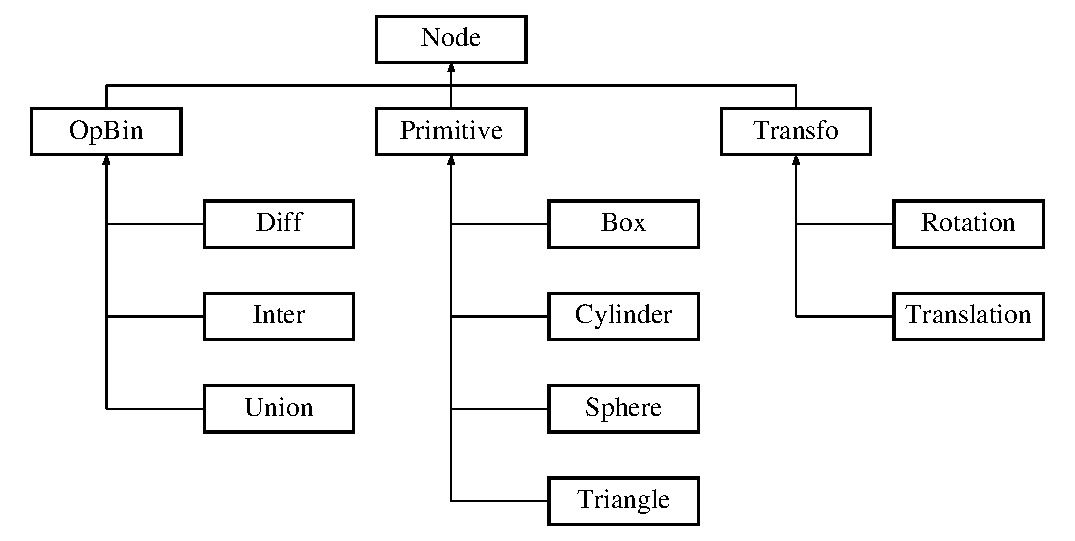
\includegraphics[height=6.000000cm]{class_node}
\end{center}
\end{figure}
\subsection*{\-Public \-Member \-Functions}
\begin{DoxyCompactItemize}
\item 
virtual int \hyperlink{class_node_ac0836475b7b0275dffe5ce89547f6852}{\-Intersect} (const \hyperlink{class_ray}{\-Ray} \&, \hyperlink{class_intersection}{\-Intersection} \&)=0
\begin{DoxyCompactList}\small\item\em \-Intersecting function. \end{DoxyCompactList}\item 
virtual int \hyperlink{class_node_a8f308647523fba2603248b83149855a5}{\-Intersect} (const \hyperlink{class_ray}{\-Ray} \&, \hyperlink{class_intersection}{\-Intersection} \&, \hyperlink{class_intersection}{\-Intersection} \&)=0
\begin{DoxyCompactList}\small\item\em \-Intersecting function. \end{DoxyCompactList}\item 
virtual int \hyperlink{class_node_aeecdf01a88be40840b65eb34cecc7a3c}{\-P\-M\-C} (const \hyperlink{class_vector}{\-Vector} \&)=0
\begin{DoxyCompactList}\small\item\em \-Containing function. \end{DoxyCompactList}\item 
\hypertarget{class_node_a3bc79b1fef701d1638b631ae384d9010}{
virtual \hyperlink{class_vector}{\-Vector} {\bfseries get\-Position} ()=0}
\label{class_node_a3bc79b1fef701d1638b631ae384d9010}

\item 
\hypertarget{class_node_ad7d3f20cd68ea44a02b0588d32cfd131}{
virtual \hyperlink{class_vector}{\-Vector} {\bfseries get\-Emission} ()=0}
\label{class_node_ad7d3f20cd68ea44a02b0588d32cfd131}

\item 
\hypertarget{class_node_aceea01792d77f81e26c83c7edc68dbe7}{
virtual \hyperlink{class_vector}{\-Vector} {\bfseries get\-Color} ()=0}
\label{class_node_aceea01792d77f81e26c83c7edc68dbe7}

\item 
\hypertarget{class_node_a1f77eb4564cc3ac5729173a48687d5b4}{
virtual double {\bfseries get\-F} ()=0}
\label{class_node_a1f77eb4564cc3ac5729173a48687d5b4}

\item 
\hypertarget{class_node_ac6efd2280f80887317b7e34b7656ac02}{
virtual int {\bfseries get\-Refl} ()=0}
\label{class_node_ac6efd2280f80887317b7e34b7656ac02}

\end{DoxyCompactItemize}


\subsection{\-Detailed \-Description}
\hyperlink{class_node}{\-Node} class. 

\hyperlink{class_node}{\-Node} is abstract class 

\subsection{\-Member \-Function \-Documentation}
\hypertarget{class_node_ac0836475b7b0275dffe5ce89547f6852}{
\index{\-Node@{\-Node}!\-Intersect@{\-Intersect}}
\index{\-Intersect@{\-Intersect}!Node@{\-Node}}
\subsubsection[{\-Intersect}]{\setlength{\rightskip}{0pt plus 5cm}virtual int \-Node\-::\-Intersect (
\begin{DoxyParamCaption}
\item[{const {\bf \-Ray} \&}]{, }
\item[{{\bf \-Intersection} \&}]{}
\end{DoxyParamCaption}
)\hspace{0.3cm}{\ttfamily  \mbox{[}pure virtual\mbox{]}}}}
\label{class_node_ac0836475b7b0275dffe5ce89547f6852}


\-Intersecting function. 

\-Compute the intersection between a node and a ray


\begin{DoxyParams}{\-Parameters}
{\em ray} & \-: the ray \\
\hline
{\em t} & \-: the intersection \\
\hline
\end{DoxyParams}


\-Implemented in \hyperlink{class_box_a6ac204afbbdc851645f33df16104292a}{\-Box}, \hyperlink{class_sphere_a4d1505b571540d40c3a6a60bd06e5fe8}{\-Sphere}, \hyperlink{class_translation_a4bd8b42e23e632d986b9b781d73676fa}{\-Translation}, \hyperlink{class_diff_a9d9ee35accad3efbed3aba5fc9da022c}{\-Diff}, \hyperlink{class_inter_a8b67290ace7c86e6cba66b5571466204}{\-Inter}, \hyperlink{class_rotation_a1209bbedf18d64a7fd7411235fb651bf}{\-Rotation}, \hyperlink{class_union_afa492095314d22df3372b4b1a3efaeca}{\-Union}, \hyperlink{class_cylinder_ac0fefa4e21c59f64bd1b52d46ffc660f}{\-Cylinder}, and \hyperlink{class_triangle_a24e02176baf3ba8b613bef47e4f416a9}{\-Triangle}.

\hypertarget{class_node_a8f308647523fba2603248b83149855a5}{
\index{\-Node@{\-Node}!\-Intersect@{\-Intersect}}
\index{\-Intersect@{\-Intersect}!Node@{\-Node}}
\subsubsection[{\-Intersect}]{\setlength{\rightskip}{0pt plus 5cm}virtual int \-Node\-::\-Intersect (
\begin{DoxyParamCaption}
\item[{const {\bf \-Ray} \&}]{, }
\item[{{\bf \-Intersection} \&}]{, }
\item[{{\bf \-Intersection} \&}]{}
\end{DoxyParamCaption}
)\hspace{0.3cm}{\ttfamily  \mbox{[}pure virtual\mbox{]}}}}
\label{class_node_a8f308647523fba2603248b83149855a5}


\-Intersecting function. 

\-Compute the intersections between a node and a ray


\begin{DoxyParams}{\-Parameters}
{\em ray} & \-: the ray \\
\hline
{\em t1} & \-: the first intersection \\
\hline
{\em t2} & \-: the second intersection \\
\hline
\end{DoxyParams}


\-Implemented in \hyperlink{class_box_a53e6a5db3bcc420700f88e6759da805d}{\-Box}, \hyperlink{class_sphere_a4199ccb2215a5c4ba1d2e80ffc842592}{\-Sphere}, \hyperlink{class_translation_aedd95cffebc575c47464090c4ac24c6f}{\-Translation}, \hyperlink{class_diff_ad2e06f30b3998b3c9592821e9a037697}{\-Diff}, \hyperlink{class_inter_a50b2aa819ddbd2c53d26e8e7342312da}{\-Inter}, \hyperlink{class_rotation_a1b1ecff10f85a2f7ab778c06e9f6f263}{\-Rotation}, \hyperlink{class_union_a2ecdc6c70bd44426bc20d88885ec497f}{\-Union}, \hyperlink{class_cylinder_ad5f756db8354800d0a95862f6de2a5fe}{\-Cylinder}, and \hyperlink{class_triangle_a4c4505c8ada8702526051f53f5a951cd}{\-Triangle}.

\hypertarget{class_node_aeecdf01a88be40840b65eb34cecc7a3c}{
\index{\-Node@{\-Node}!\-P\-M\-C@{\-P\-M\-C}}
\index{\-P\-M\-C@{\-P\-M\-C}!Node@{\-Node}}
\subsubsection[{\-P\-M\-C}]{\setlength{\rightskip}{0pt plus 5cm}virtual int \-Node\-::\-P\-M\-C (
\begin{DoxyParamCaption}
\item[{const {\bf \-Vector} \&}]{}
\end{DoxyParamCaption}
)\hspace{0.3cm}{\ttfamily  \mbox{[}pure virtual\mbox{]}}}}
\label{class_node_aeecdf01a88be40840b65eb34cecc7a3c}


\-Containing function. 

\-Checks if the point is inside the instance


\begin{DoxyParams}{\-Parameters}
{\em u} & \-: the point \\
\hline
\end{DoxyParams}


\-Implemented in \hyperlink{class_box_afb71788385a4f8ff91c6d8385972dde4}{\-Box}, \hyperlink{class_sphere_abccfe78233b90c14e6e2afe74e27e6d5}{\-Sphere}, \hyperlink{class_translation_a23217f05d1442f4f5fc7db511dd57434}{\-Translation}, \hyperlink{class_diff_a9569764d64e3cc072c554ceffad7934a}{\-Diff}, \hyperlink{class_inter_a62fb756b8848c042f6ea48bbe204f4a6}{\-Inter}, \hyperlink{class_rotation_a1dbfa88ef89ea7bd50a875ca7fe9f911}{\-Rotation}, \hyperlink{class_union_ae9430083fcfdc62199b26db6e511d150}{\-Union}, \hyperlink{class_cylinder_a54d8f47f574488e583868fbd5dfd9abf}{\-Cylinder}, and \hyperlink{class_triangle_ab6066a8828559d40c1f88dfcf92723bb}{\-Triangle}.



\-The documentation for this class was generated from the following file\-:\begin{DoxyCompactItemize}
\item 
headers/\hyperlink{node_8h}{node.\-h}\end{DoxyCompactItemize}

\hypertarget{class_op_bin}{
\section{\-Op\-Bin \-Class \-Reference}
\label{class_op_bin}\index{\-Op\-Bin@{\-Op\-Bin}}
}


\hyperlink{class_op_bin}{\-Op\-Bin} class.  




{\ttfamily \#include $<$opbin.\-h$>$}

\-Inheritance diagram for \-Op\-Bin\-:\begin{figure}[H]
\begin{center}
\leavevmode
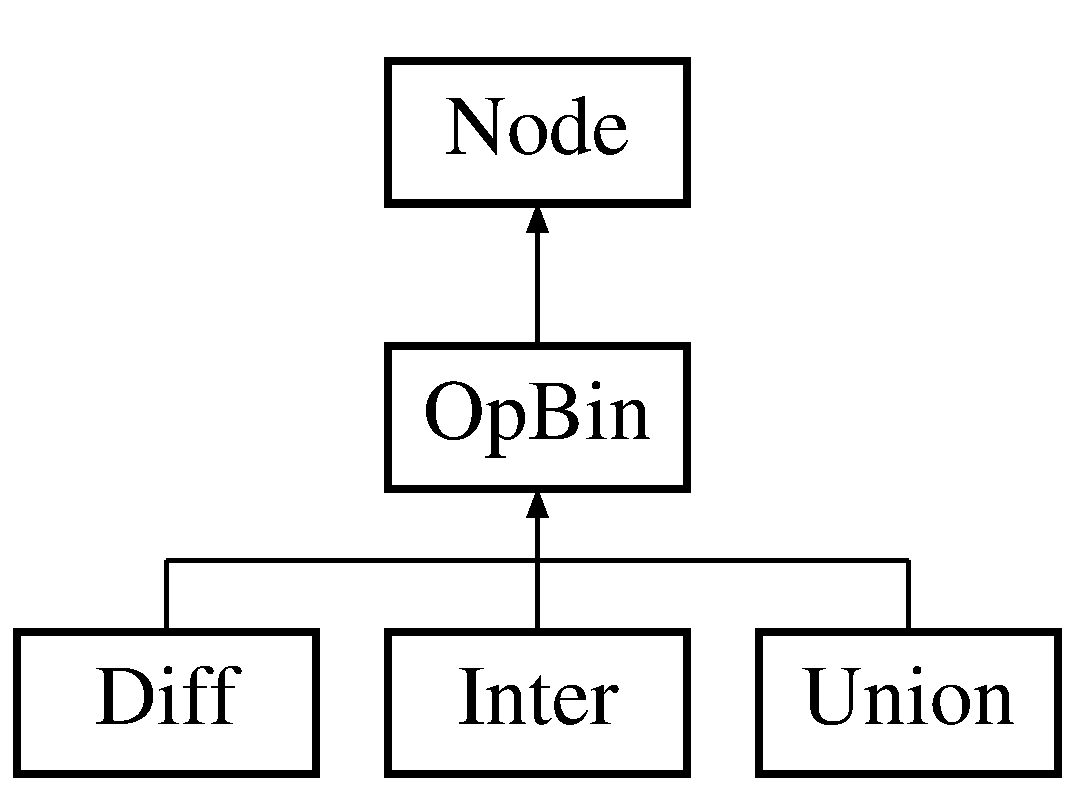
\includegraphics[height=3.000000cm]{class_op_bin}
\end{center}
\end{figure}
\subsection*{\-Public \-Member \-Functions}
\begin{DoxyCompactItemize}
\item 
\hypertarget{class_op_bin_a9dbb8dfeff7846ea176eb6ceb72cd729}{
{\bfseries \-Op\-Bin} (\hyperlink{class_node}{\-Node} $\ast$, \hyperlink{class_node}{\-Node} $\ast$)}
\label{class_op_bin_a9dbb8dfeff7846ea176eb6ceb72cd729}

\end{DoxyCompactItemize}
\subsection*{\-Protected \-Attributes}
\begin{DoxyCompactItemize}
\item 
\hyperlink{class_node}{\-Node} $\ast$ \hyperlink{class_op_bin_a5f5db8a000a36f5c609313d0d880ed61}{left}
\item 
\hyperlink{class_node}{\-Node} $\ast$ \hyperlink{class_op_bin_a1c79a6c7464203dbf5aa7167dfbdb301}{right}
\end{DoxyCompactItemize}


\subsection{\-Detailed \-Description}
\hyperlink{class_op_bin}{\-Op\-Bin} class. 

\hyperlink{class_op_bin}{\-Op\-Bin} is a operand with two primitives 

\subsection{\-Member \-Data \-Documentation}
\hypertarget{class_op_bin_a5f5db8a000a36f5c609313d0d880ed61}{
\index{\-Op\-Bin@{\-Op\-Bin}!left@{left}}
\index{left@{left}!OpBin@{\-Op\-Bin}}
\subsubsection[{left}]{\setlength{\rightskip}{0pt plus 5cm}{\bf \-Node}$\ast$ {\bf \-Op\-Bin\-::left}\hspace{0.3cm}{\ttfamily  \mbox{[}protected\mbox{]}}}}
\label{class_op_bin_a5f5db8a000a36f5c609313d0d880ed61}
\-Left element of the operation \hypertarget{class_op_bin_a1c79a6c7464203dbf5aa7167dfbdb301}{
\index{\-Op\-Bin@{\-Op\-Bin}!right@{right}}
\index{right@{right}!OpBin@{\-Op\-Bin}}
\subsubsection[{right}]{\setlength{\rightskip}{0pt plus 5cm}{\bf \-Node}$\ast$ {\bf \-Op\-Bin\-::right}\hspace{0.3cm}{\ttfamily  \mbox{[}protected\mbox{]}}}}
\label{class_op_bin_a1c79a6c7464203dbf5aa7167dfbdb301}
\-Right element of the operation 

\-The documentation for this class was generated from the following file\-:\begin{DoxyCompactItemize}
\item 
headers/\hyperlink{opbin_8h}{opbin.\-h}\end{DoxyCompactItemize}

\hypertarget{class_primitive}{
\section{\-Primitive \-Class \-Reference}
\label{class_primitive}\index{\-Primitive@{\-Primitive}}
}


\hyperlink{class_primitive}{\-Primitive} class.  




{\ttfamily \#include $<$primitive.\-h$>$}

\-Inheritance diagram for \-Primitive\-:\begin{figure}[H]
\begin{center}
\leavevmode
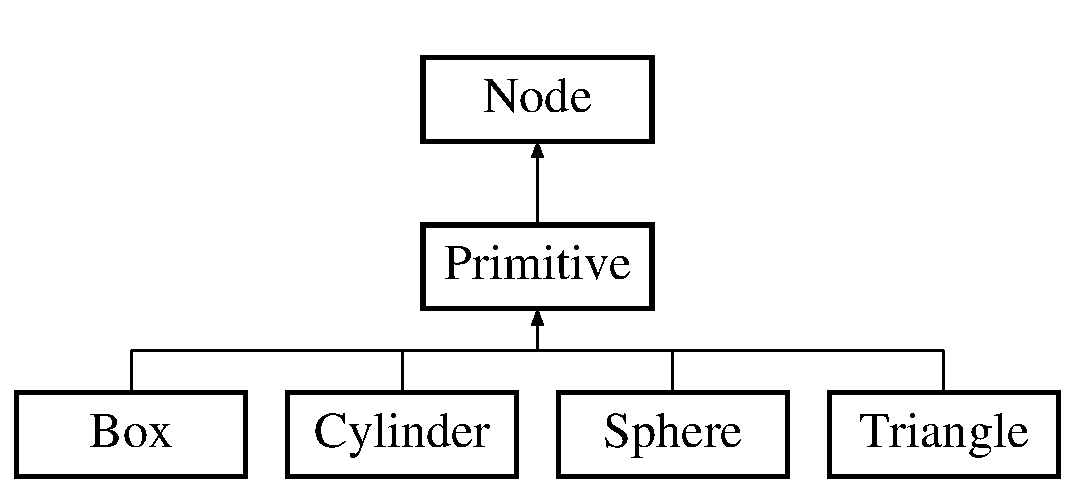
\includegraphics[height=3.000000cm]{class_primitive}
\end{center}
\end{figure}
\subsection*{\-Public \-Member \-Functions}
\begin{DoxyCompactItemize}
\item 
\hypertarget{class_primitive_a91a5e120794dfe52e920c75a1bff0008}{
{\bfseries \-Primitive} (const \hyperlink{class_vector}{\-Vector} \&, const \hyperlink{class_vector}{\-Vector} \&, int)}
\label{class_primitive_a91a5e120794dfe52e920c75a1bff0008}

\item 
\hypertarget{class_primitive_a1a0a0c026a30397c23944b4270fdfbc0}{
\hyperlink{class_vector}{\-Vector} {\bfseries get\-Emission} ()}
\label{class_primitive_a1a0a0c026a30397c23944b4270fdfbc0}

\item 
\hypertarget{class_primitive_ae092397067c2197f62f70ab930146f3a}{
\hyperlink{class_vector}{\-Vector} {\bfseries get\-Color} ()}
\label{class_primitive_ae092397067c2197f62f70ab930146f3a}

\item 
\hypertarget{class_primitive_acc17c8f82c1e434be04c1d13aaccb69c}{
int {\bfseries get\-Refl} ()}
\label{class_primitive_acc17c8f82c1e434be04c1d13aaccb69c}

\item 
\hypertarget{class_primitive_ab0f0642b9a163d32462be8e8edcb30ff}{
double {\bfseries get\-F} ()}
\label{class_primitive_ab0f0642b9a163d32462be8e8edcb30ff}

\end{DoxyCompactItemize}
\subsection*{\-Protected \-Attributes}
\begin{DoxyCompactItemize}
\item 
\hyperlink{class_vector}{\-Vector} \hyperlink{class_primitive_aa60d41fbc09fbf11f6dd24b6e0252c5d}{e}
\item 
\hyperlink{class_vector}{\-Vector} \hyperlink{class_primitive_a3952aadb4a03a2e98e6ba5bdfbd0842f}{c}
\item 
int \hyperlink{class_primitive_a39a03ec4e90d63a30e1594b4d396fa77}{refl}
\item 
double \hyperlink{class_primitive_a6e6c2ea0ddfaaca10a3b18bb08af0706}{f}
\end{DoxyCompactItemize}


\subsection{\-Detailed \-Description}
\hyperlink{class_primitive}{\-Primitive} class. 

\hyperlink{class_primitive}{\-Primitive} is a kind of node 

\subsection{\-Member \-Data \-Documentation}
\hypertarget{class_primitive_a3952aadb4a03a2e98e6ba5bdfbd0842f}{
\index{\-Primitive@{\-Primitive}!c@{c}}
\index{c@{c}!Primitive@{\-Primitive}}
\subsubsection[{c}]{\setlength{\rightskip}{0pt plus 5cm}{\bf \-Vector} {\bf \-Primitive\-::c}\hspace{0.3cm}{\ttfamily  \mbox{[}protected\mbox{]}}}}
\label{class_primitive_a3952aadb4a03a2e98e6ba5bdfbd0842f}
\-Color \hypertarget{class_primitive_aa60d41fbc09fbf11f6dd24b6e0252c5d}{
\index{\-Primitive@{\-Primitive}!e@{e}}
\index{e@{e}!Primitive@{\-Primitive}}
\subsubsection[{e}]{\setlength{\rightskip}{0pt plus 5cm}{\bf \-Vector} {\bf \-Primitive\-::e}\hspace{0.3cm}{\ttfamily  \mbox{[}protected\mbox{]}}}}
\label{class_primitive_aa60d41fbc09fbf11f6dd24b6e0252c5d}
\-Emission \hypertarget{class_primitive_a6e6c2ea0ddfaaca10a3b18bb08af0706}{
\index{\-Primitive@{\-Primitive}!f@{f}}
\index{f@{f}!Primitive@{\-Primitive}}
\subsubsection[{f}]{\setlength{\rightskip}{0pt plus 5cm}double {\bf \-Primitive\-::f}\hspace{0.3cm}{\ttfamily  \mbox{[}protected\mbox{]}}}}
\label{class_primitive_a6e6c2ea0ddfaaca10a3b18bb08af0706}
\-Maximum color channel value \hypertarget{class_primitive_a39a03ec4e90d63a30e1594b4d396fa77}{
\index{\-Primitive@{\-Primitive}!refl@{refl}}
\index{refl@{refl}!Primitive@{\-Primitive}}
\subsubsection[{refl}]{\setlength{\rightskip}{0pt plus 5cm}int {\bf \-Primitive\-::refl}\hspace{0.3cm}{\ttfamily  \mbox{[}protected\mbox{]}}}}
\label{class_primitive_a39a03ec4e90d63a30e1594b4d396fa77}
\-Reflection type 

\-The documentation for this class was generated from the following file\-:\begin{DoxyCompactItemize}
\item 
headers/\hyperlink{primitive_8h}{primitive.\-h}\end{DoxyCompactItemize}

\hypertarget{class_ray}{
\section{\-Ray \-Class \-Reference}
\label{class_ray}\index{\-Ray@{\-Ray}}
}


\hyperlink{class_ray}{\-Ray} class.  




{\ttfamily \#include $<$ray.\-h$>$}

\subsection*{\-Public \-Member \-Functions}
\begin{DoxyCompactItemize}
\item 
\hyperlink{class_ray_ac042e01bad2bc40d7b82782d606d73bc}{\-Ray} (const \hyperlink{class_vector}{\-Vector} \&, const \hyperlink{class_vector}{\-Vector} \&)
\begin{DoxyCompactList}\small\item\em \hyperlink{class_ray}{\-Ray} constructor. \end{DoxyCompactList}\item 
\hypertarget{class_ray_ac7370340c4d068b895e96197affbdd55}{
\hyperlink{class_ray}{\-Ray} {\bfseries \-Reflect} (const \hyperlink{class_vector}{\-Vector} \&, const \hyperlink{class_vector}{\-Vector} \&) const }
\label{class_ray_ac7370340c4d068b895e96197affbdd55}

\item 
\hyperlink{class_vector}{\-Vector} \hyperlink{class_ray_a001ec0c1257895bfd10cd707f17b10b7}{operator()} (const double \&t) const 
\begin{DoxyCompactList}\small\item\em \-Computes the location of a vertex along the ray. \end{DoxyCompactList}\item 
\hypertarget{class_ray_a1f64bed4515cb96aadbe4d0e5f86458f}{
\hyperlink{class_vector}{\-Vector} {\bfseries \-Origin} () const }
\label{class_ray_a1f64bed4515cb96aadbe4d0e5f86458f}

\item 
\hypertarget{class_ray_a03b73a4709636a9a2c526c569265f84e}{
\hyperlink{class_vector}{\-Vector} {\bfseries \-Direction} () const }
\label{class_ray_a03b73a4709636a9a2c526c569265f84e}

\end{DoxyCompactItemize}
\subsection*{\-Protected \-Attributes}
\begin{DoxyCompactItemize}
\item 
\hyperlink{class_vector}{\-Vector} \hyperlink{class_ray_a2e41a40406edbbb3103ca0734a435c08}{c}
\item 
\hyperlink{class_vector}{\-Vector} \hyperlink{class_ray_a70e0d3a943faf00a399e432c386fd146}{n}
\end{DoxyCompactItemize}


\subsection{\-Detailed \-Description}
\hyperlink{class_ray}{\-Ray} class. 

\hyperlink{class_ray}{\-Ray} is a data structure 

\subsection{\-Constructor \& \-Destructor \-Documentation}
\hypertarget{class_ray_ac042e01bad2bc40d7b82782d606d73bc}{
\index{\-Ray@{\-Ray}!\-Ray@{\-Ray}}
\index{\-Ray@{\-Ray}!Ray@{\-Ray}}
\subsubsection[{\-Ray}]{\setlength{\rightskip}{0pt plus 5cm}\-Ray\-::\-Ray (
\begin{DoxyParamCaption}
\item[{const {\bf \-Vector} \&}]{p, }
\item[{const {\bf \-Vector} \&}]{d}
\end{DoxyParamCaption}
)\hspace{0.3cm}{\ttfamily  \mbox{[}inline\mbox{]}}}}
\label{class_ray_ac042e01bad2bc40d7b82782d606d73bc}


\hyperlink{class_ray}{\-Ray} constructor. 


\begin{DoxyParams}{\-Parameters}
{\em p} & \-: \-Origin \\
\hline
{\em d} & \-: \-Direction \\
\hline
\end{DoxyParams}


\subsection{\-Member \-Function \-Documentation}
\hypertarget{class_ray_a001ec0c1257895bfd10cd707f17b10b7}{
\index{\-Ray@{\-Ray}!operator()@{operator()}}
\index{operator()@{operator()}!Ray@{\-Ray}}
\subsubsection[{operator()}]{\setlength{\rightskip}{0pt plus 5cm}{\bf \-Vector} \-Ray\-::operator() (
\begin{DoxyParamCaption}
\item[{const double \&}]{t}
\end{DoxyParamCaption}
) const\hspace{0.3cm}{\ttfamily  \mbox{[}inline\mbox{]}}}}
\label{class_ray_a001ec0c1257895bfd10cd707f17b10b7}


\-Computes the location of a vertex along the ray. 


\begin{DoxyParams}{\-Parameters}
{\em t} & \-: \-Distance between the ray origin and the vertex \\
\hline
\end{DoxyParams}


\subsection{\-Member \-Data \-Documentation}
\hypertarget{class_ray_a2e41a40406edbbb3103ca0734a435c08}{
\index{\-Ray@{\-Ray}!c@{c}}
\index{c@{c}!Ray@{\-Ray}}
\subsubsection[{c}]{\setlength{\rightskip}{0pt plus 5cm}{\bf \-Vector} {\bf \-Ray\-::c}\hspace{0.3cm}{\ttfamily  \mbox{[}protected\mbox{]}}}}
\label{class_ray_a2e41a40406edbbb3103ca0734a435c08}
\-Origin of the ray \hypertarget{class_ray_a70e0d3a943faf00a399e432c386fd146}{
\index{\-Ray@{\-Ray}!n@{n}}
\index{n@{n}!Ray@{\-Ray}}
\subsubsection[{n}]{\setlength{\rightskip}{0pt plus 5cm}{\bf \-Vector} {\bf \-Ray\-::n}\hspace{0.3cm}{\ttfamily  \mbox{[}protected\mbox{]}}}}
\label{class_ray_a70e0d3a943faf00a399e432c386fd146}
\-Direction 

\-The documentation for this class was generated from the following file\-:\begin{DoxyCompactItemize}
\item 
headers/\hyperlink{ray_8h}{ray.\-h}\end{DoxyCompactItemize}

\hypertarget{class_rotation}{
\section{\-Rotation \-Class \-Reference}
\label{class_rotation}\index{\-Rotation@{\-Rotation}}
}


\hyperlink{class_rotation}{\-Rotation} class.  




{\ttfamily \#include $<$rotation.\-h$>$}

\-Inheritance diagram for \-Rotation\-:\begin{figure}[H]
\begin{center}
\leavevmode
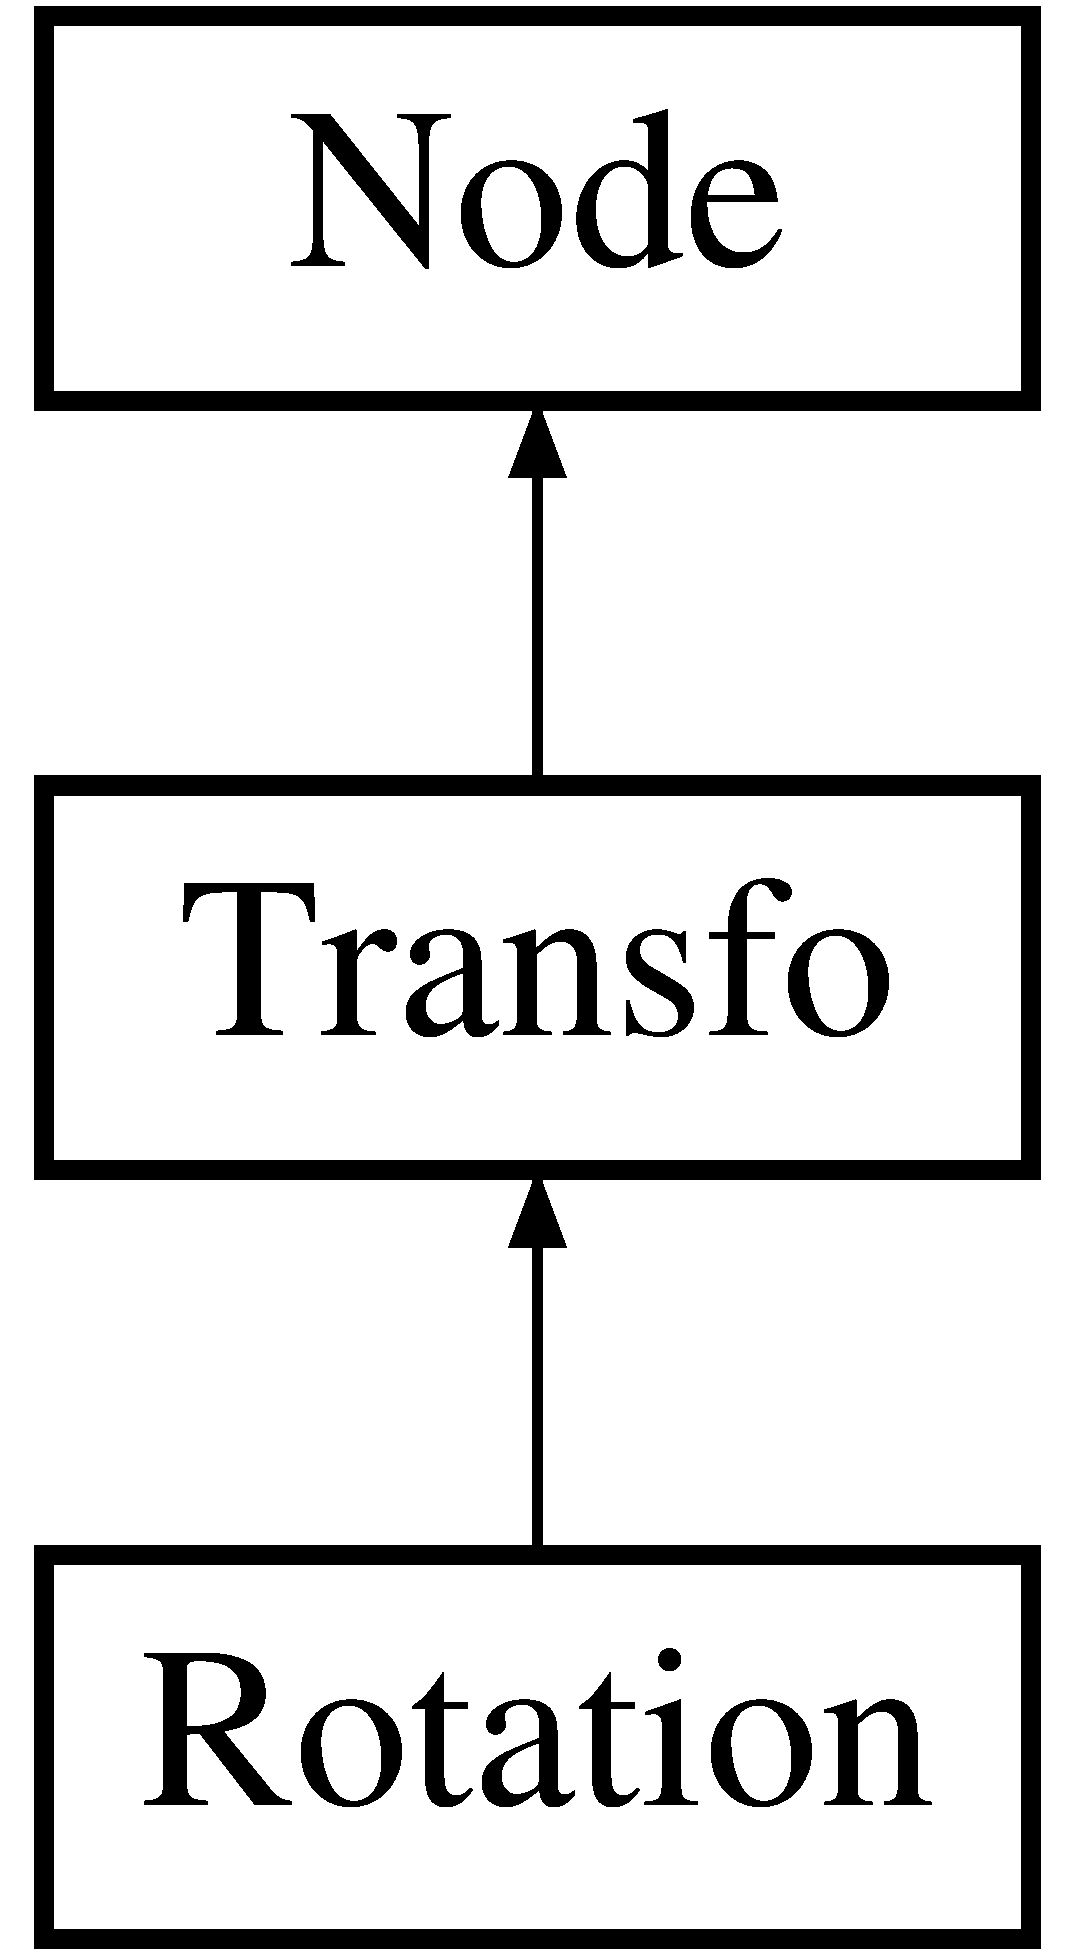
\includegraphics[height=3.000000cm]{class_rotation}
\end{center}
\end{figure}
\subsection*{\-Public \-Member \-Functions}
\begin{DoxyCompactItemize}
\item 
\hypertarget{class_rotation_a19ef7fb0baa64a4a518923f5c831fdd2}{
{\bfseries \-Rotation} (\hyperlink{class_node}{\-Node} $\ast$, const \hyperlink{class_vector}{\-Vector}, float angle)}
\label{class_rotation_a19ef7fb0baa64a4a518923f5c831fdd2}

\item 
int \hyperlink{class_rotation_a1209bbedf18d64a7fd7411235fb651bf}{\-Intersect} (const \hyperlink{class_ray}{\-Ray} \&, \hyperlink{class_intersection}{\-Intersection} \&)
\begin{DoxyCompactList}\small\item\em \-Intersecting function. \end{DoxyCompactList}\item 
int \hyperlink{class_rotation_a1b1ecff10f85a2f7ab778c06e9f6f263}{\-Intersect} (const \hyperlink{class_ray}{\-Ray} \&, \hyperlink{class_intersection}{\-Intersection} \&, \hyperlink{class_intersection}{\-Intersection} \&)
\begin{DoxyCompactList}\small\item\em \-Intersecting function. \end{DoxyCompactList}\item 
int \hyperlink{class_rotation_a1dbfa88ef89ea7bd50a875ca7fe9f911}{\-P\-M\-C} (const \hyperlink{class_vector}{\-Vector} \&)
\begin{DoxyCompactList}\small\item\em \-Containing function. \end{DoxyCompactList}\item 
\hypertarget{class_rotation_a16df69dc33ea554cfde8c8fa2d0174f2}{
\hyperlink{class_vector}{\-Vector} {\bfseries get\-Emission} ()}
\label{class_rotation_a16df69dc33ea554cfde8c8fa2d0174f2}

\item 
\hypertarget{class_rotation_a15418e82c782df1687eb2dd11cc469eb}{
\hyperlink{class_vector}{\-Vector} {\bfseries get\-Color} ()}
\label{class_rotation_a15418e82c782df1687eb2dd11cc469eb}

\item 
\hypertarget{class_rotation_a3dd8b11ab6ff47d626e49d766702210c}{
\hyperlink{class_vector}{\-Vector} {\bfseries get\-Position} ()}
\label{class_rotation_a3dd8b11ab6ff47d626e49d766702210c}

\item 
\hypertarget{class_rotation_acd09beb7679985b103b4e638deae0904}{
int {\bfseries get\-Refl} ()}
\label{class_rotation_acd09beb7679985b103b4e638deae0904}

\item 
\hypertarget{class_rotation_acea503033dd5293b86e3481682f6b29b}{
double {\bfseries get\-F} ()}
\label{class_rotation_acea503033dd5293b86e3481682f6b29b}

\end{DoxyCompactItemize}
\subsection*{\-Public \-Attributes}
\begin{DoxyCompactItemize}
\item 
\hypertarget{class_rotation_a3abe27c3f55eefef38dd5097485a3b2b}{
\hyperlink{class_matrix4_df}{\-Matrix4\-Df} {\bfseries m\-Rotate}}
\label{class_rotation_a3abe27c3f55eefef38dd5097485a3b2b}

\item 
\hypertarget{class_rotation_a3a6d1397aaa3ed90101e705747ebf19a}{
\hyperlink{class_matrix4_df}{\-Matrix4\-Df} {\bfseries m\-Rotate\-Inv}}
\label{class_rotation_a3a6d1397aaa3ed90101e705747ebf19a}

\end{DoxyCompactItemize}


\subsection{\-Detailed \-Description}
\hyperlink{class_rotation}{\-Rotation} class. 

\hyperlink{class_rotation}{\-Rotation} is a transformation for the \-C\-S\-G 

\subsection{\-Member \-Function \-Documentation}
\hypertarget{class_rotation_a1209bbedf18d64a7fd7411235fb651bf}{
\index{\-Rotation@{\-Rotation}!\-Intersect@{\-Intersect}}
\index{\-Intersect@{\-Intersect}!Rotation@{\-Rotation}}
\subsubsection[{\-Intersect}]{\setlength{\rightskip}{0pt plus 5cm}int \-Rotation\-::\-Intersect (
\begin{DoxyParamCaption}
\item[{const {\bf \-Ray} \&}]{, }
\item[{{\bf \-Intersection} \&}]{}
\end{DoxyParamCaption}
)\hspace{0.3cm}{\ttfamily  \mbox{[}virtual\mbox{]}}}}
\label{class_rotation_a1209bbedf18d64a7fd7411235fb651bf}


\-Intersecting function. 

\-Compute the intersection between a rotation and a ray


\begin{DoxyParams}{\-Parameters}
{\em ray} & \-: the ray \\
\hline
{\em t} & \-: the intersection \\
\hline
\end{DoxyParams}


\-Implements \hyperlink{class_node_ac0836475b7b0275dffe5ce89547f6852}{\-Node}.

\hypertarget{class_rotation_a1b1ecff10f85a2f7ab778c06e9f6f263}{
\index{\-Rotation@{\-Rotation}!\-Intersect@{\-Intersect}}
\index{\-Intersect@{\-Intersect}!Rotation@{\-Rotation}}
\subsubsection[{\-Intersect}]{\setlength{\rightskip}{0pt plus 5cm}int \-Rotation\-::\-Intersect (
\begin{DoxyParamCaption}
\item[{const {\bf \-Ray} \&}]{, }
\item[{{\bf \-Intersection} \&}]{, }
\item[{{\bf \-Intersection} \&}]{}
\end{DoxyParamCaption}
)\hspace{0.3cm}{\ttfamily  \mbox{[}virtual\mbox{]}}}}
\label{class_rotation_a1b1ecff10f85a2f7ab778c06e9f6f263}


\-Intersecting function. 

\-Compute the intersections between a rotation and a ray


\begin{DoxyParams}{\-Parameters}
{\em ray} & \-: the ray \\
\hline
{\em t} & \-: the first intersection \\
\hline
{\em t2} & \-: the second intersection \\
\hline
\end{DoxyParams}


\-Implements \hyperlink{class_node_a8f308647523fba2603248b83149855a5}{\-Node}.

\hypertarget{class_rotation_a1dbfa88ef89ea7bd50a875ca7fe9f911}{
\index{\-Rotation@{\-Rotation}!\-P\-M\-C@{\-P\-M\-C}}
\index{\-P\-M\-C@{\-P\-M\-C}!Rotation@{\-Rotation}}
\subsubsection[{\-P\-M\-C}]{\setlength{\rightskip}{0pt plus 5cm}int \-Rotation\-::\-P\-M\-C (
\begin{DoxyParamCaption}
\item[{const {\bf \-Vector} \&}]{}
\end{DoxyParamCaption}
)\hspace{0.3cm}{\ttfamily  \mbox{[}virtual\mbox{]}}}}
\label{class_rotation_a1dbfa88ef89ea7bd50a875ca7fe9f911}


\-Containing function. 

\-Checks if a point is inside the instance


\begin{DoxyParams}{\-Parameters}
{\em u} & \-: the point \\
\hline
\end{DoxyParams}


\-Implements \hyperlink{class_node_aeecdf01a88be40840b65eb34cecc7a3c}{\-Node}.



\-The documentation for this class was generated from the following file\-:\begin{DoxyCompactItemize}
\item 
headers/\hyperlink{rotation_8h}{rotation.\-h}\end{DoxyCompactItemize}

\hypertarget{class_sphere}{
\section{\-Sphere \-Class \-Reference}
\label{class_sphere}\index{\-Sphere@{\-Sphere}}
}


\hyperlink{class_sphere}{\-Sphere} class.  




{\ttfamily \#include $<$sphere.\-h$>$}

\-Inheritance diagram for \-Sphere\-:\begin{figure}[H]
\begin{center}
\leavevmode
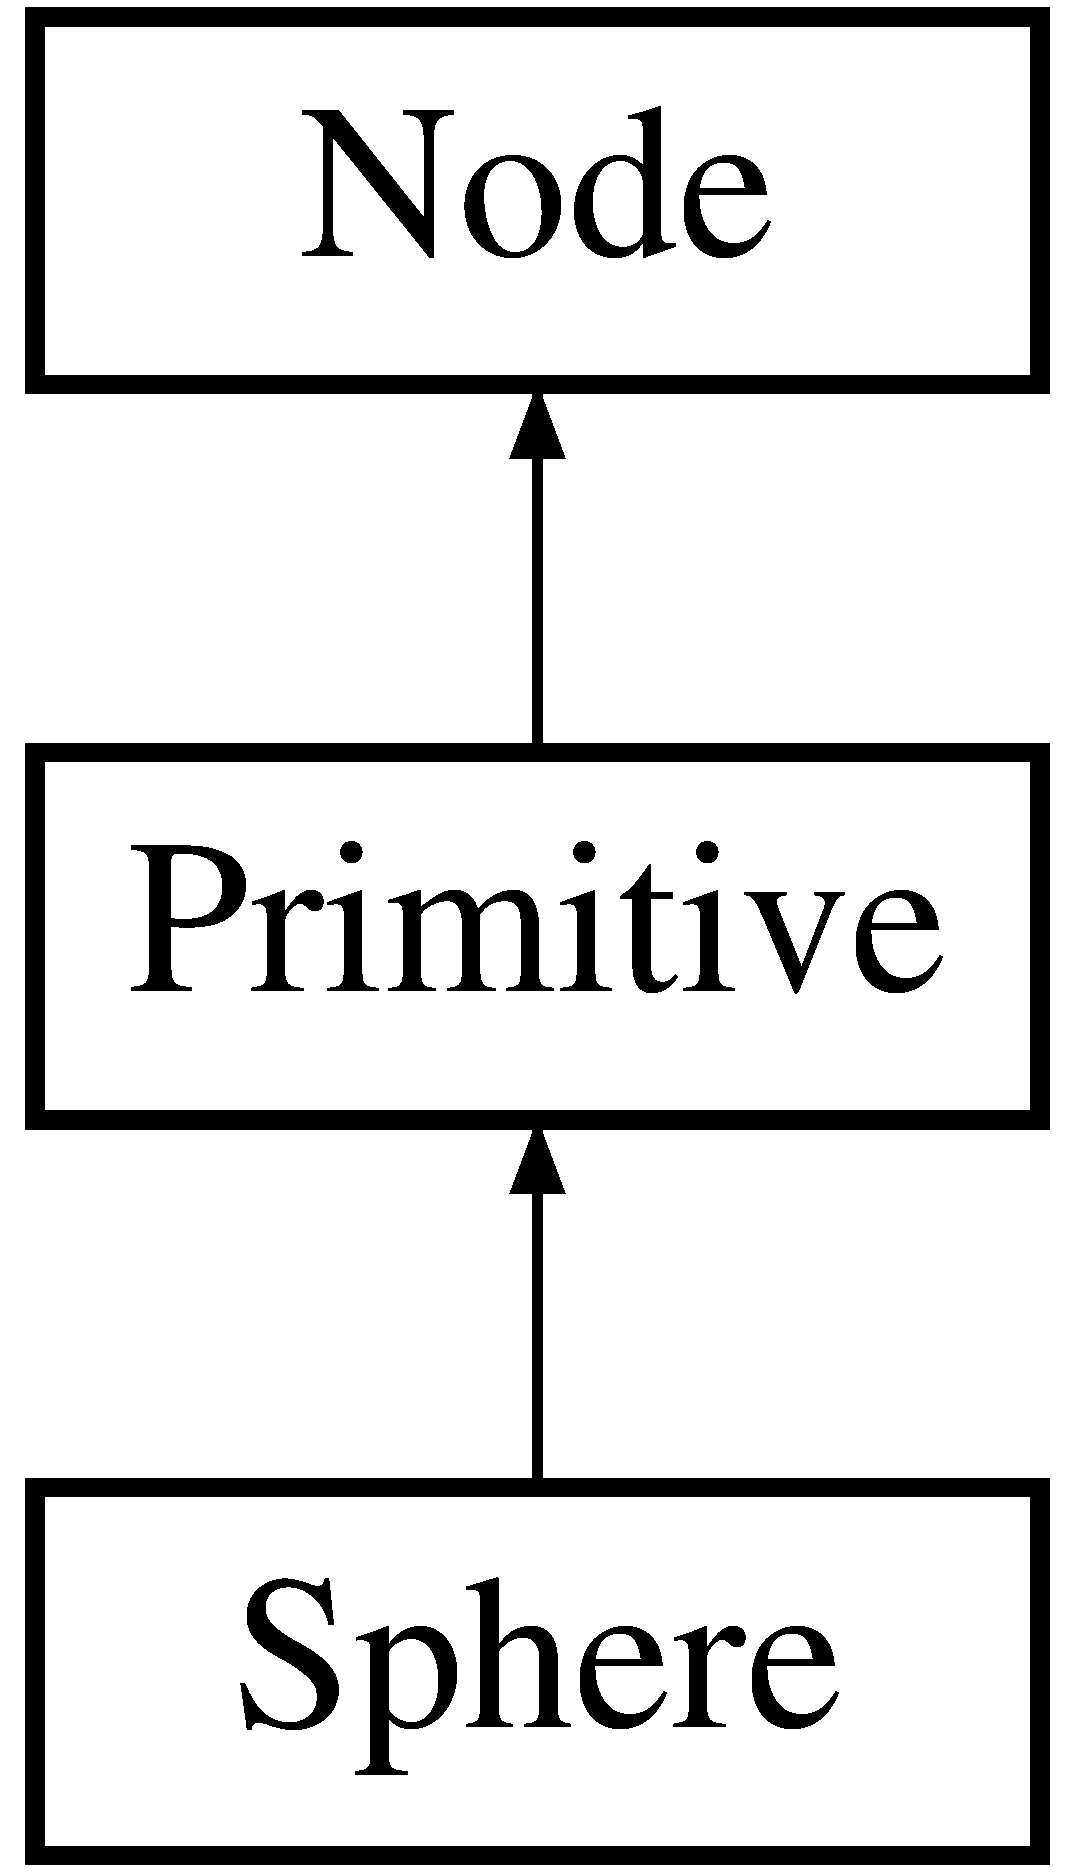
\includegraphics[height=3.000000cm]{class_sphere}
\end{center}
\end{figure}
\subsection*{\-Public \-Member \-Functions}
\begin{DoxyCompactItemize}
\item 
\hypertarget{class_sphere_ae1b26180ec6543e7705c69dc680a54b5}{
{\bfseries \-Sphere} (const double \&, const \hyperlink{class_vector}{\-Vector} \&, const \hyperlink{class_vector}{\-Vector} \&, const \hyperlink{class_vector}{\-Vector} \&, int)}
\label{class_sphere_ae1b26180ec6543e7705c69dc680a54b5}

\item 
int \hyperlink{class_sphere_a4d1505b571540d40c3a6a60bd06e5fe8}{\-Intersect} (const \hyperlink{class_ray}{\-Ray} \&r, \hyperlink{class_intersection}{\-Intersection} \&)
\begin{DoxyCompactList}\small\item\em \-Intersecting function. \end{DoxyCompactList}\item 
int \hyperlink{class_sphere_a4199ccb2215a5c4ba1d2e80ffc842592}{\-Intersect} (const \hyperlink{class_ray}{\-Ray} \&, \hyperlink{class_intersection}{\-Intersection} \&, \hyperlink{class_intersection}{\-Intersection} \&)
\begin{DoxyCompactList}\small\item\em \-Intersecting function. \end{DoxyCompactList}\item 
int \hyperlink{class_sphere_abccfe78233b90c14e6e2afe74e27e6d5}{\-P\-M\-C} (const \hyperlink{class_vector}{\-Vector} \&)
\begin{DoxyCompactList}\small\item\em \-Containing function. \end{DoxyCompactList}\item 
\hypertarget{class_sphere_af1989cb4d1c48de8e2f90c7e9ef21db8}{
\hyperlink{class_vector}{\-Vector} {\bfseries get\-Position} ()}
\label{class_sphere_af1989cb4d1c48de8e2f90c7e9ef21db8}

\end{DoxyCompactItemize}
\subsection*{\-Public \-Attributes}
\begin{DoxyCompactItemize}
\item 
\hypertarget{class_sphere_a78176ca986a3d21fe84fbff0a82e2ed1}{
double \hyperlink{class_sphere_a78176ca986a3d21fe84fbff0a82e2ed1}{rad}}
\label{class_sphere_a78176ca986a3d21fe84fbff0a82e2ed1}

\begin{DoxyCompactList}\small\item\em \-Radius. \end{DoxyCompactList}\item 
\hypertarget{class_sphere_a66360df163b9107d8ee28b67a41fe4af}{
\hyperlink{class_vector}{\-Vector} \hyperlink{class_sphere_a66360df163b9107d8ee28b67a41fe4af}{p}}
\label{class_sphere_a66360df163b9107d8ee28b67a41fe4af}

\begin{DoxyCompactList}\small\item\em position, emission, color \end{DoxyCompactList}\end{DoxyCompactItemize}


\subsection{\-Detailed \-Description}
\hyperlink{class_sphere}{\-Sphere} class. 

\hyperlink{class_sphere}{\-Sphere} is a primitive of the \-C\-S\-G 

\subsection{\-Member \-Function \-Documentation}
\hypertarget{class_sphere_a4d1505b571540d40c3a6a60bd06e5fe8}{
\index{\-Sphere@{\-Sphere}!\-Intersect@{\-Intersect}}
\index{\-Intersect@{\-Intersect}!Sphere@{\-Sphere}}
\subsubsection[{\-Intersect}]{\setlength{\rightskip}{0pt plus 5cm}int \-Sphere\-::\-Intersect (
\begin{DoxyParamCaption}
\item[{const {\bf \-Ray} \&}]{r, }
\item[{{\bf \-Intersection} \&}]{}
\end{DoxyParamCaption}
)\hspace{0.3cm}{\ttfamily  \mbox{[}virtual\mbox{]}}}}
\label{class_sphere_a4d1505b571540d40c3a6a60bd06e5fe8}


\-Intersecting function. 

\-Compute the intersection between a sphere and a ray


\begin{DoxyParams}{\-Parameters}
{\em ray} & \-: the ray \\
\hline
{\em inter} & \-: the intersection \\
\hline
\end{DoxyParams}


\-Implements \hyperlink{class_node_ac0836475b7b0275dffe5ce89547f6852}{\-Node}.

\hypertarget{class_sphere_a4199ccb2215a5c4ba1d2e80ffc842592}{
\index{\-Sphere@{\-Sphere}!\-Intersect@{\-Intersect}}
\index{\-Intersect@{\-Intersect}!Sphere@{\-Sphere}}
\subsubsection[{\-Intersect}]{\setlength{\rightskip}{0pt plus 5cm}int \-Sphere\-::\-Intersect (
\begin{DoxyParamCaption}
\item[{const {\bf \-Ray} \&}]{, }
\item[{{\bf \-Intersection} \&}]{, }
\item[{{\bf \-Intersection} \&}]{}
\end{DoxyParamCaption}
)\hspace{0.3cm}{\ttfamily  \mbox{[}virtual\mbox{]}}}}
\label{class_sphere_a4199ccb2215a5c4ba1d2e80ffc842592}


\-Intersecting function. 

\-Compute the intersections between a sphere and a ray


\begin{DoxyParams}{\-Parameters}
{\em ray} & \-: the ray \\
\hline
{\em intermin} & \-: the first intersection \\
\hline
{\em intermax} & \-: the second intersection \\
\hline
\end{DoxyParams}


\-Implements \hyperlink{class_node_a8f308647523fba2603248b83149855a5}{\-Node}.

\hypertarget{class_sphere_abccfe78233b90c14e6e2afe74e27e6d5}{
\index{\-Sphere@{\-Sphere}!\-P\-M\-C@{\-P\-M\-C}}
\index{\-P\-M\-C@{\-P\-M\-C}!Sphere@{\-Sphere}}
\subsubsection[{\-P\-M\-C}]{\setlength{\rightskip}{0pt plus 5cm}int \-Sphere\-::\-P\-M\-C (
\begin{DoxyParamCaption}
\item[{const {\bf \-Vector} \&}]{}
\end{DoxyParamCaption}
)\hspace{0.3cm}{\ttfamily  \mbox{[}virtual\mbox{]}}}}
\label{class_sphere_abccfe78233b90c14e6e2afe74e27e6d5}


\-Containing function. 

\-Checks if a point is inside the instance


\begin{DoxyParams}{\-Parameters}
{\em a} & \-: the point \\
\hline
\end{DoxyParams}


\-Implements \hyperlink{class_node_aeecdf01a88be40840b65eb34cecc7a3c}{\-Node}.



\-The documentation for this class was generated from the following file\-:\begin{DoxyCompactItemize}
\item 
headers/\hyperlink{sphere_8h}{sphere.\-h}\end{DoxyCompactItemize}

\hypertarget{class_transfo}{
\section{\-Transfo \-Class \-Reference}
\label{class_transfo}\index{\-Transfo@{\-Transfo}}
}


\hyperlink{class_transfo}{\-Transfo} class.  




{\ttfamily \#include $<$transfo.\-h$>$}

\-Inheritance diagram for \-Transfo\-:\begin{figure}[H]
\begin{center}
\leavevmode
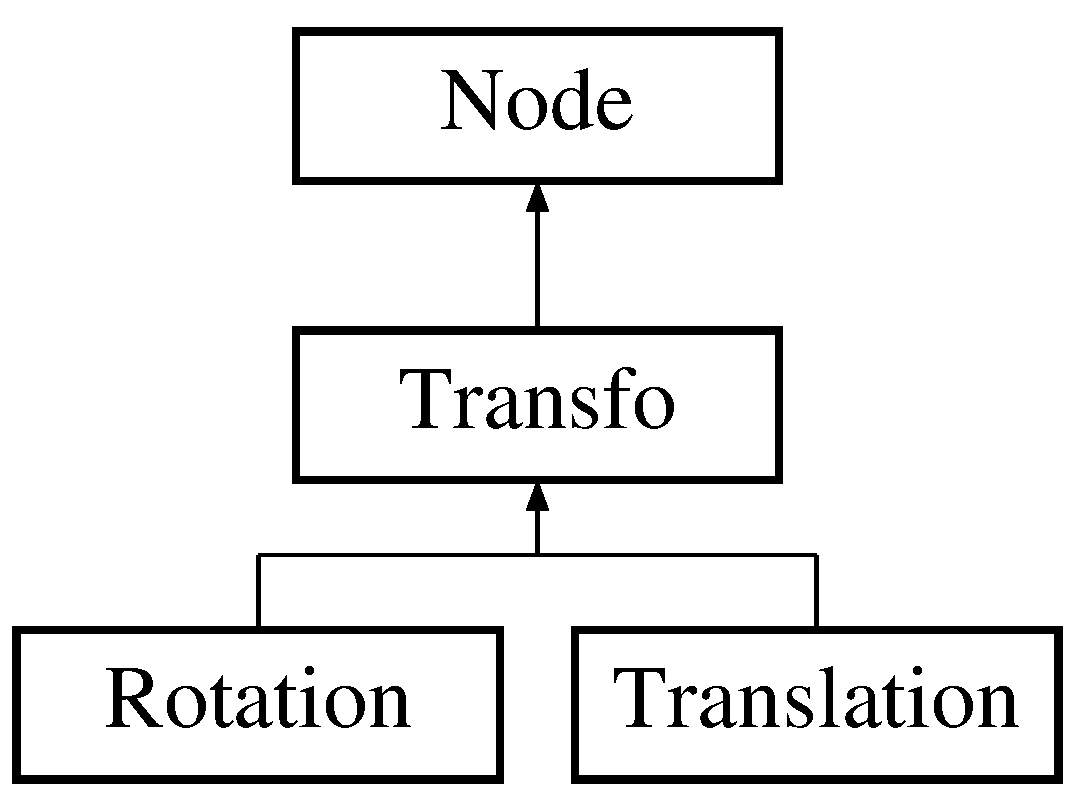
\includegraphics[height=3.000000cm]{class_transfo}
\end{center}
\end{figure}
\subsection*{\-Public \-Member \-Functions}
\begin{DoxyCompactItemize}
\item 
\hypertarget{class_transfo_a37b1c80234fdd7bb1e8f6191baf1a03c}{
{\bfseries \-Transfo} (\hyperlink{class_node}{\-Node} $\ast$l)}
\label{class_transfo_a37b1c80234fdd7bb1e8f6191baf1a03c}

\end{DoxyCompactItemize}
\subsection*{\-Protected \-Attributes}
\begin{DoxyCompactItemize}
\item 
\hypertarget{class_transfo_a09757e6952c70b4c5d533f76937cd01c}{
\hyperlink{class_node}{\-Node} $\ast$ {\bfseries left}}
\label{class_transfo_a09757e6952c70b4c5d533f76937cd01c}

\item 
\hypertarget{class_transfo_aadda74e44474e62e2d530dbc51ddfe84}{
\hyperlink{class_node}{\-Node} $\ast$ {\bfseries right}}
\label{class_transfo_aadda74e44474e62e2d530dbc51ddfe84}

\item 
\hypertarget{class_transfo_a4b903a28698fd3697f18e9df9e829372}{
\hyperlink{class_matrix4_df}{\-Matrix4\-Df} {\bfseries m}}
\label{class_transfo_a4b903a28698fd3697f18e9df9e829372}

\item 
\hypertarget{class_transfo_aab329728f1f9ba1f270c438990021eb8}{
\hyperlink{class_matrix4_df}{\-Matrix4\-Df} {\bfseries m\-Inv}}
\label{class_transfo_aab329728f1f9ba1f270c438990021eb8}

\end{DoxyCompactItemize}


\subsection{\-Detailed \-Description}
\hyperlink{class_transfo}{\-Transfo} class. 

\hyperlink{class_transfo}{\-Transfo} is a kind of node 

\-The documentation for this class was generated from the following file\-:\begin{DoxyCompactItemize}
\item 
headers/\hyperlink{transfo_8h}{transfo.\-h}\end{DoxyCompactItemize}

\hypertarget{class_translation}{
\section{\-Translation \-Class \-Reference}
\label{class_translation}\index{\-Translation@{\-Translation}}
}


\hyperlink{class_translation}{\-Translation} class.  




{\ttfamily \#include $<$translation.\-h$>$}

\-Inheritance diagram for \-Translation\-:\begin{figure}[H]
\begin{center}
\leavevmode
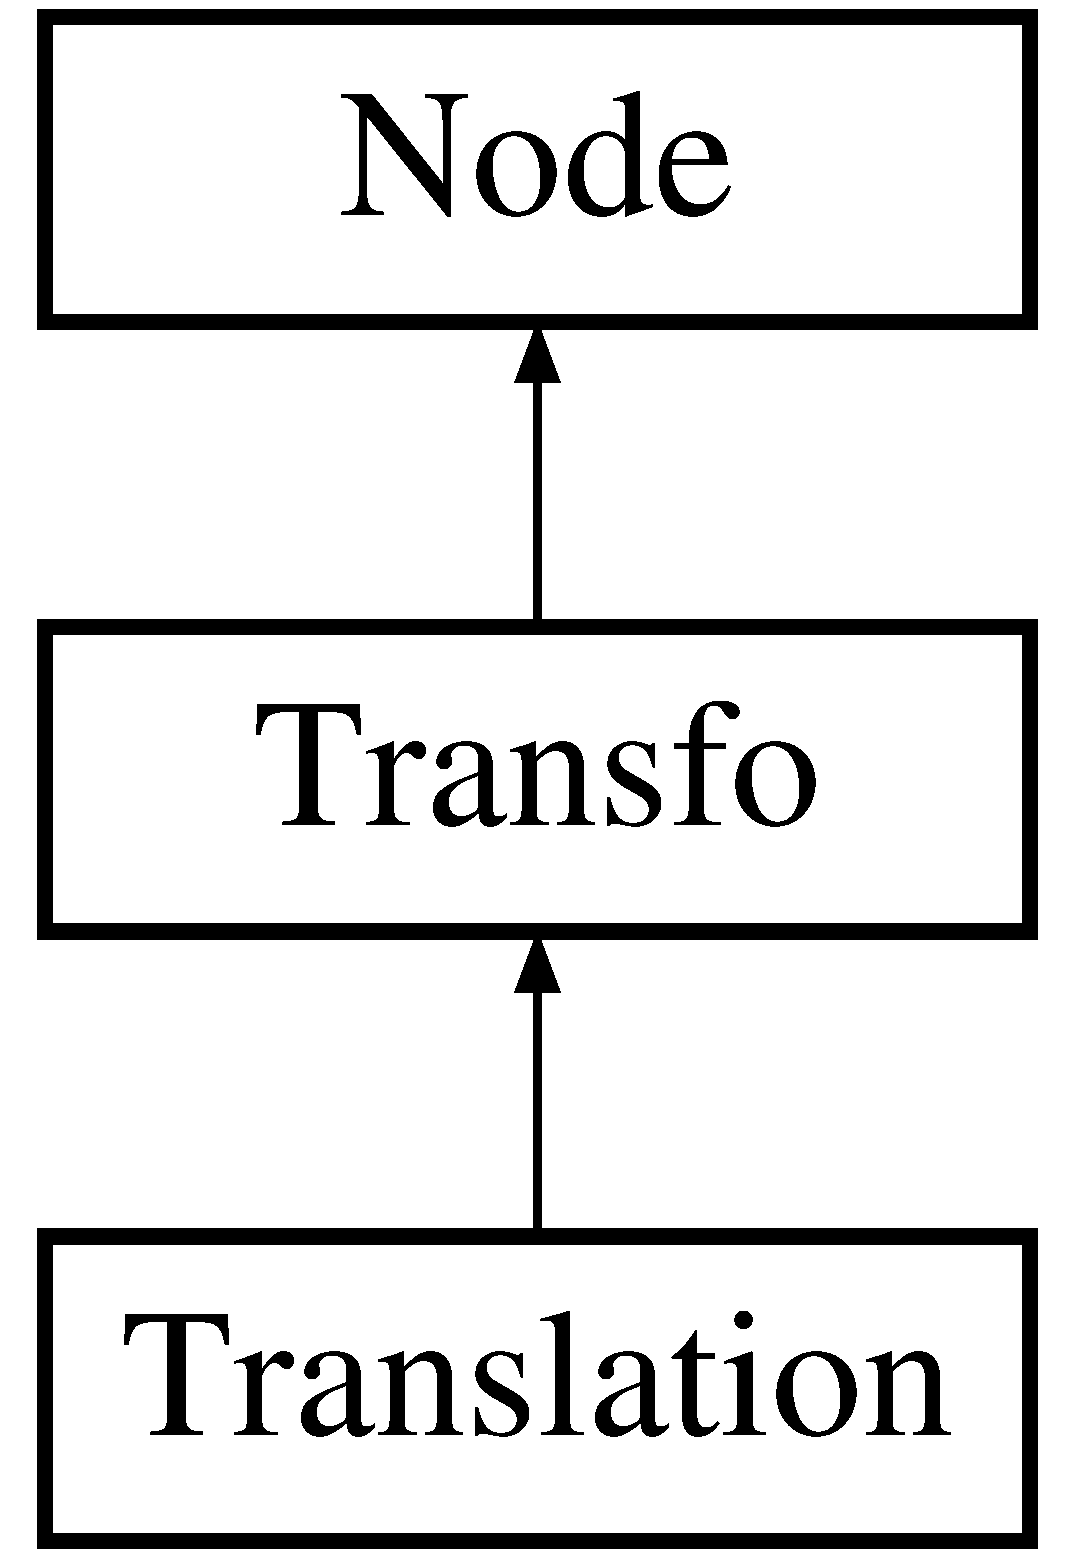
\includegraphics[height=3.000000cm]{class_translation}
\end{center}
\end{figure}
\subsection*{\-Public \-Member \-Functions}
\begin{DoxyCompactItemize}
\item 
\hypertarget{class_translation_a1ecd9177ce516202fe010b47ef007265}{
{\bfseries \-Translation} (\hyperlink{class_node}{\-Node} $\ast$, const \hyperlink{class_vector}{\-Vector})}
\label{class_translation_a1ecd9177ce516202fe010b47ef007265}

\item 
int \hyperlink{class_translation_a4bd8b42e23e632d986b9b781d73676fa}{\-Intersect} (const \hyperlink{class_ray}{\-Ray} \&, \hyperlink{class_intersection}{\-Intersection} \&)
\begin{DoxyCompactList}\small\item\em \-Intersecting function. \end{DoxyCompactList}\item 
int \hyperlink{class_translation_aedd95cffebc575c47464090c4ac24c6f}{\-Intersect} (const \hyperlink{class_ray}{\-Ray} \&, \hyperlink{class_intersection}{\-Intersection} \&, \hyperlink{class_intersection}{\-Intersection} \&)
\begin{DoxyCompactList}\small\item\em \-Intersecting function. \end{DoxyCompactList}\item 
int \hyperlink{class_translation_a23217f05d1442f4f5fc7db511dd57434}{\-P\-M\-C} (const \hyperlink{class_vector}{\-Vector} \&)
\begin{DoxyCompactList}\small\item\em \-Containing function. \end{DoxyCompactList}\item 
\hypertarget{class_translation_af54c9803dfefa1ec04c13a40daedb823}{
\hyperlink{class_vector}{\-Vector} {\bfseries get\-Emission} ()}
\label{class_translation_af54c9803dfefa1ec04c13a40daedb823}

\item 
\hypertarget{class_translation_abdb54c49d261e8770d1d12119542fc1b}{
\hyperlink{class_vector}{\-Vector} {\bfseries get\-Color} ()}
\label{class_translation_abdb54c49d261e8770d1d12119542fc1b}

\item 
\hypertarget{class_translation_a27c4202120108256e3f5cbc940d619b1}{
\hyperlink{class_vector}{\-Vector} {\bfseries get\-Position} ()}
\label{class_translation_a27c4202120108256e3f5cbc940d619b1}

\item 
\hypertarget{class_translation_ae2dce5d15431d1a602dc763ebe615495}{
int {\bfseries get\-Refl} ()}
\label{class_translation_ae2dce5d15431d1a602dc763ebe615495}

\item 
\hypertarget{class_translation_aeefc7fa602cd2eb815f1a9c06f1d4d0c}{
double {\bfseries get\-F} ()}
\label{class_translation_aeefc7fa602cd2eb815f1a9c06f1d4d0c}

\end{DoxyCompactItemize}


\subsection{\-Detailed \-Description}
\hyperlink{class_translation}{\-Translation} class. 

\hyperlink{class_translation}{\-Translation} is a transformation for the \-C\-S\-G 

\subsection{\-Member \-Function \-Documentation}
\hypertarget{class_translation_a4bd8b42e23e632d986b9b781d73676fa}{
\index{\-Translation@{\-Translation}!\-Intersect@{\-Intersect}}
\index{\-Intersect@{\-Intersect}!Translation@{\-Translation}}
\subsubsection[{\-Intersect}]{\setlength{\rightskip}{0pt plus 5cm}int \-Translation\-::\-Intersect (
\begin{DoxyParamCaption}
\item[{const {\bf \-Ray} \&}]{, }
\item[{{\bf \-Intersection} \&}]{}
\end{DoxyParamCaption}
)\hspace{0.3cm}{\ttfamily  \mbox{[}virtual\mbox{]}}}}
\label{class_translation_a4bd8b42e23e632d986b9b781d73676fa}


\-Intersecting function. 

\-Compute the intersection between a translation and a ray


\begin{DoxyParams}{\-Parameters}
{\em ray} & \-: the ray \\
\hline
{\em t} & \-: the intersection \\
\hline
\end{DoxyParams}


\-Implements \hyperlink{class_node_ac0836475b7b0275dffe5ce89547f6852}{\-Node}.

\hypertarget{class_translation_aedd95cffebc575c47464090c4ac24c6f}{
\index{\-Translation@{\-Translation}!\-Intersect@{\-Intersect}}
\index{\-Intersect@{\-Intersect}!Translation@{\-Translation}}
\subsubsection[{\-Intersect}]{\setlength{\rightskip}{0pt plus 5cm}int \-Translation\-::\-Intersect (
\begin{DoxyParamCaption}
\item[{const {\bf \-Ray} \&}]{, }
\item[{{\bf \-Intersection} \&}]{, }
\item[{{\bf \-Intersection} \&}]{}
\end{DoxyParamCaption}
)\hspace{0.3cm}{\ttfamily  \mbox{[}virtual\mbox{]}}}}
\label{class_translation_aedd95cffebc575c47464090c4ac24c6f}


\-Intersecting function. 

\-Compute the intersections between a translation and a ray


\begin{DoxyParams}{\-Parameters}
{\em ray} & \-: the ray \\
\hline
{\em t} & \-: the first intersection \\
\hline
{\em t2} & \-: the second intersection \\
\hline
\end{DoxyParams}


\-Implements \hyperlink{class_node_a8f308647523fba2603248b83149855a5}{\-Node}.

\hypertarget{class_translation_a23217f05d1442f4f5fc7db511dd57434}{
\index{\-Translation@{\-Translation}!\-P\-M\-C@{\-P\-M\-C}}
\index{\-P\-M\-C@{\-P\-M\-C}!Translation@{\-Translation}}
\subsubsection[{\-P\-M\-C}]{\setlength{\rightskip}{0pt plus 5cm}int \-Translation\-::\-P\-M\-C (
\begin{DoxyParamCaption}
\item[{const {\bf \-Vector} \&}]{}
\end{DoxyParamCaption}
)\hspace{0.3cm}{\ttfamily  \mbox{[}virtual\mbox{]}}}}
\label{class_translation_a23217f05d1442f4f5fc7db511dd57434}


\-Containing function. 

\-Checks if a point is inside the instance


\begin{DoxyParams}{\-Parameters}
{\em u} & \-: the point \\
\hline
\end{DoxyParams}


\-Implements \hyperlink{class_node_aeecdf01a88be40840b65eb34cecc7a3c}{\-Node}.



\-The documentation for this class was generated from the following file\-:\begin{DoxyCompactItemize}
\item 
headers/\hyperlink{translation_8h}{translation.\-h}\end{DoxyCompactItemize}

\hypertarget{class_triangle}{
\section{\-Triangle \-Class \-Reference}
\label{class_triangle}\index{\-Triangle@{\-Triangle}}
}


\hyperlink{class_triangle}{\-Triangle} class.  




{\ttfamily \#include $<$triangle.\-h$>$}

\-Inheritance diagram for \-Triangle\-:\begin{figure}[H]
\begin{center}
\leavevmode
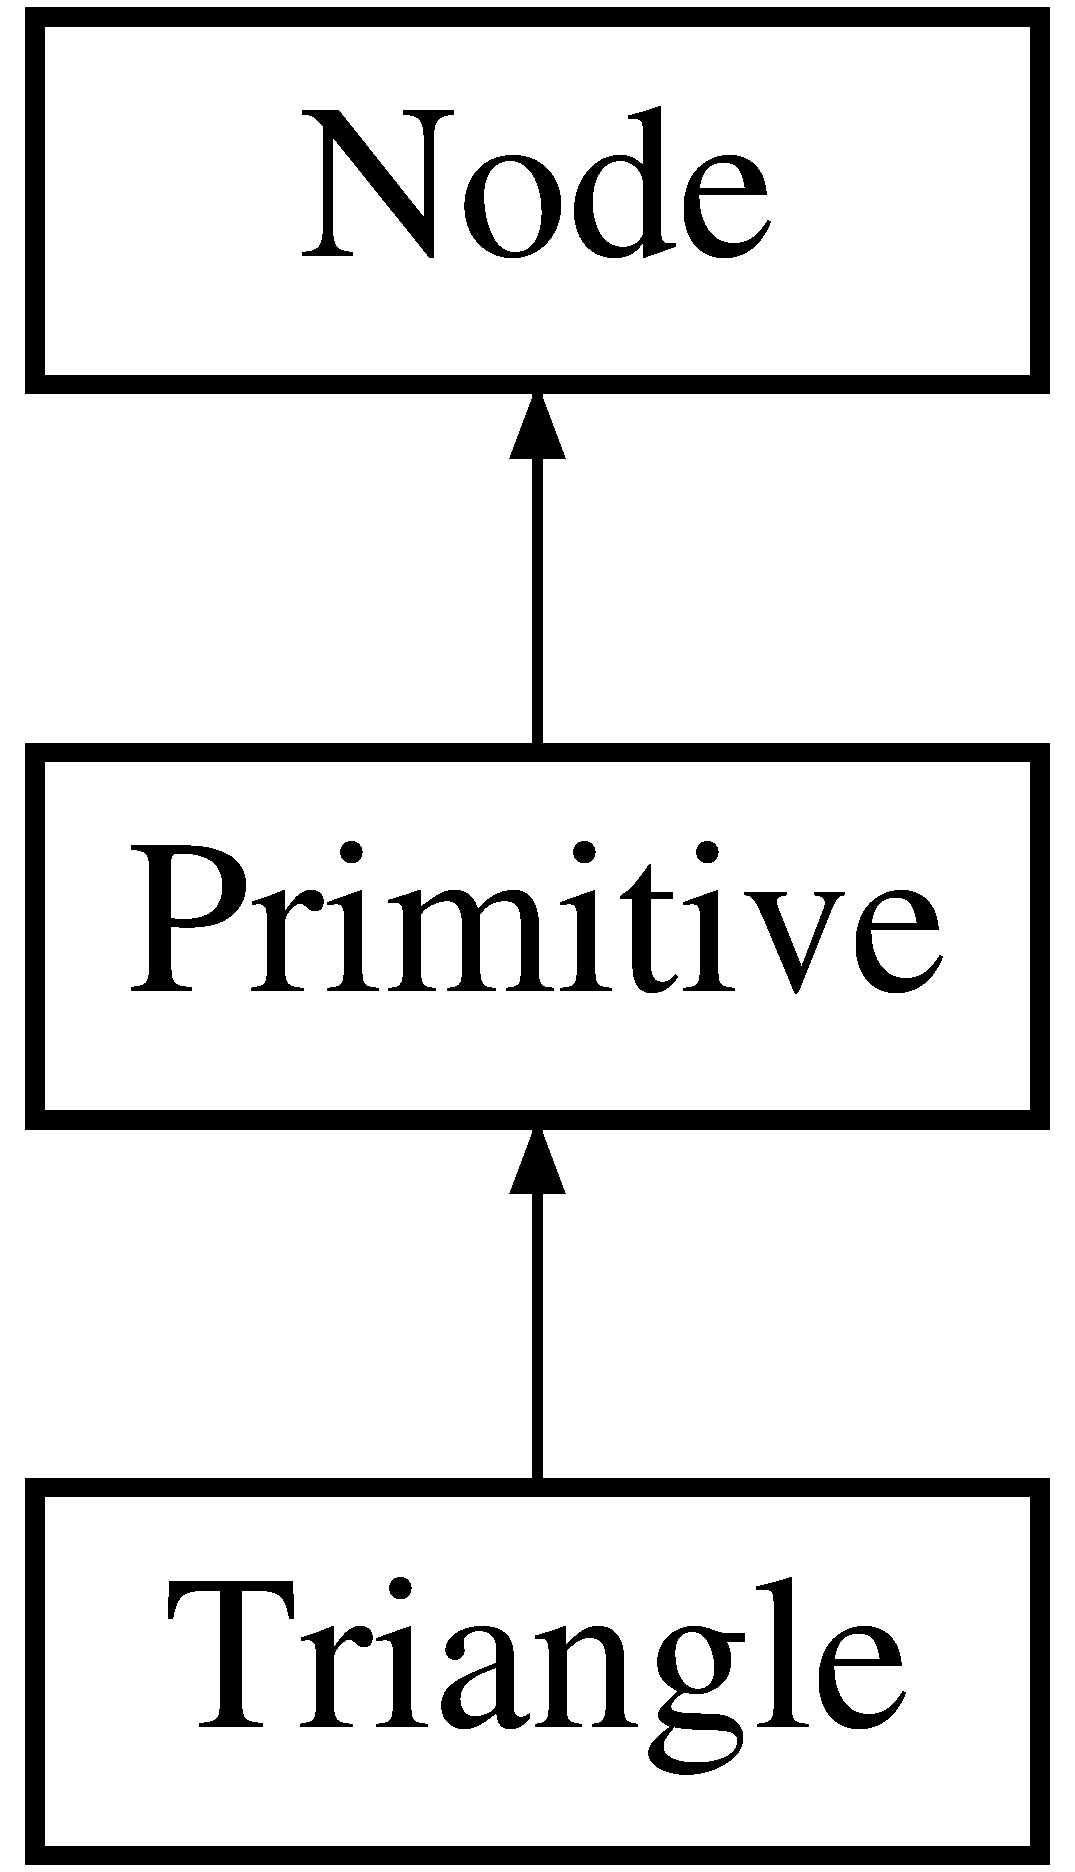
\includegraphics[height=3.000000cm]{class_triangle}
\end{center}
\end{figure}
\subsection*{\-Public \-Member \-Functions}
\begin{DoxyCompactItemize}
\item 
\hypertarget{class_triangle_a793ed45b623e913b5ea59799a29a2ebf}{
{\bfseries \-Triangle} (const \hyperlink{class_vector}{\-Vector} \&, const \hyperlink{class_vector}{\-Vector} \&, const \hyperlink{class_vector}{\-Vector} \&, const \hyperlink{class_vector}{\-Vector} \&, const \hyperlink{class_vector}{\-Vector} \&, int)}
\label{class_triangle_a793ed45b623e913b5ea59799a29a2ebf}

\item 
int \hyperlink{class_triangle_a24e02176baf3ba8b613bef47e4f416a9}{\-Intersect} (const \hyperlink{class_ray}{\-Ray} \&, \hyperlink{class_intersection}{\-Intersection} \&)
\begin{DoxyCompactList}\small\item\em \-Intersecting function. \end{DoxyCompactList}\item 
int \hyperlink{class_triangle_a4c4505c8ada8702526051f53f5a951cd}{\-Intersect} (const \hyperlink{class_ray}{\-Ray} \&, \hyperlink{class_intersection}{\-Intersection} \&, \hyperlink{class_intersection}{\-Intersection} \&)
\begin{DoxyCompactList}\small\item\em \-Intersecting function. \end{DoxyCompactList}\item 
int \hyperlink{class_triangle_ab6066a8828559d40c1f88dfcf92723bb}{\-P\-M\-C} (const \hyperlink{class_vector}{\-Vector} \&)
\begin{DoxyCompactList}\small\item\em \-P\-M\-C function. \end{DoxyCompactList}\item 
\hyperlink{class_vector}{\-Vector} \hyperlink{class_triangle_ad26a8346e3d5f5c65c3e982d8e1f260e}{get\-Position} ()
\begin{DoxyCompactList}\small\item\em \-Get position function. \end{DoxyCompactList}\end{DoxyCompactItemize}
\subsection*{\-Protected \-Attributes}
\begin{DoxyCompactItemize}
\item 
\hyperlink{class_vector}{\-Vector} \hyperlink{class_triangle_adebd4b41a74691d5da67db5c8f852672}{p1}
\item 
\hyperlink{class_vector}{\-Vector} \hyperlink{class_triangle_a7bba48c61a088c93914768018b2329af}{p2}
\item 
\hyperlink{class_vector}{\-Vector} \hyperlink{class_triangle_a7df8e8ed225f77daee7e5eb4bf5b9f99}{p3}
\end{DoxyCompactItemize}


\subsection{\-Detailed \-Description}
\hyperlink{class_triangle}{\-Triangle} class. 

\hyperlink{class_triangle}{\-Triangle} is a primitive of the \-C\-S\-G 

\subsection{\-Member \-Function \-Documentation}
\hypertarget{class_triangle_ad26a8346e3d5f5c65c3e982d8e1f260e}{
\index{\-Triangle@{\-Triangle}!get\-Position@{get\-Position}}
\index{get\-Position@{get\-Position}!Triangle@{\-Triangle}}
\subsubsection[{get\-Position}]{\setlength{\rightskip}{0pt plus 5cm}{\bf \-Vector} \-Triangle\-::get\-Position (
\begin{DoxyParamCaption}
{}
\end{DoxyParamCaption}
)\hspace{0.3cm}{\ttfamily  \mbox{[}virtual\mbox{]}}}}
\label{class_triangle_ad26a8346e3d5f5c65c3e982d8e1f260e}


\-Get position function. 

\-Compute the triangle position 

\-Implements \hyperlink{class_node}{\-Node}.

\hypertarget{class_triangle_a24e02176baf3ba8b613bef47e4f416a9}{
\index{\-Triangle@{\-Triangle}!\-Intersect@{\-Intersect}}
\index{\-Intersect@{\-Intersect}!Triangle@{\-Triangle}}
\subsubsection[{\-Intersect}]{\setlength{\rightskip}{0pt plus 5cm}int \-Triangle\-::\-Intersect (
\begin{DoxyParamCaption}
\item[{const {\bf \-Ray} \&}]{, }
\item[{{\bf \-Intersection} \&}]{}
\end{DoxyParamCaption}
)\hspace{0.3cm}{\ttfamily  \mbox{[}virtual\mbox{]}}}}
\label{class_triangle_a24e02176baf3ba8b613bef47e4f416a9}


\-Intersecting function. 

\-Compute the intersection between a node and a ray


\begin{DoxyParams}{\-Parameters}
{\em ray} & \-: the ray \\
\hline
{\em t} & \-: the intersection \\
\hline
\end{DoxyParams}


\-Implements \hyperlink{class_node_ac0836475b7b0275dffe5ce89547f6852}{\-Node}.

\hypertarget{class_triangle_a4c4505c8ada8702526051f53f5a951cd}{
\index{\-Triangle@{\-Triangle}!\-Intersect@{\-Intersect}}
\index{\-Intersect@{\-Intersect}!Triangle@{\-Triangle}}
\subsubsection[{\-Intersect}]{\setlength{\rightskip}{0pt plus 5cm}int \-Triangle\-::\-Intersect (
\begin{DoxyParamCaption}
\item[{const {\bf \-Ray} \&}]{, }
\item[{{\bf \-Intersection} \&}]{, }
\item[{{\bf \-Intersection} \&}]{}
\end{DoxyParamCaption}
)\hspace{0.3cm}{\ttfamily  \mbox{[}virtual\mbox{]}}}}
\label{class_triangle_a4c4505c8ada8702526051f53f5a951cd}


\-Intersecting function. 

\-Compute the intersections between a triangle and a ray


\begin{DoxyParams}{\-Parameters}
{\em ray} & \-: the ray \\
\hline
{\em inter1} & \-: the first intersection \\
\hline
{\em inter2} & \-: the second intersection \\
\hline
\end{DoxyParams}


\-Implements \hyperlink{class_node_a8f308647523fba2603248b83149855a5}{\-Node}.

\hypertarget{class_triangle_ab6066a8828559d40c1f88dfcf92723bb}{
\index{\-Triangle@{\-Triangle}!\-P\-M\-C@{\-P\-M\-C}}
\index{\-P\-M\-C@{\-P\-M\-C}!Triangle@{\-Triangle}}
\subsubsection[{\-P\-M\-C}]{\setlength{\rightskip}{0pt plus 5cm}int \-Triangle\-::\-P\-M\-C (
\begin{DoxyParamCaption}
\item[{const {\bf \-Vector} \&}]{}
\end{DoxyParamCaption}
)\hspace{0.3cm}{\ttfamily  \mbox{[}virtual\mbox{]}}}}
\label{class_triangle_ab6066a8828559d40c1f88dfcf92723bb}


\-P\-M\-C function. 

\-Compute if the point is in the triangle


\begin{DoxyParams}{\-Parameters}
{\em point} & \-: the point \\
\hline
\end{DoxyParams}


\-Implements \hyperlink{class_node_aeecdf01a88be40840b65eb34cecc7a3c}{\-Node}.



\subsection{\-Member \-Data \-Documentation}
\hypertarget{class_triangle_adebd4b41a74691d5da67db5c8f852672}{
\index{\-Triangle@{\-Triangle}!p1@{p1}}
\index{p1@{p1}!Triangle@{\-Triangle}}
\subsubsection[{p1}]{\setlength{\rightskip}{0pt plus 5cm}{\bf \-Vector} {\bf \-Triangle\-::p1}\hspace{0.3cm}{\ttfamily  \mbox{[}protected\mbox{]}}}}
\label{class_triangle_adebd4b41a74691d5da67db5c8f852672}
\hyperlink{class_triangle}{\-Triangle} point p1 \hypertarget{class_triangle_a7bba48c61a088c93914768018b2329af}{
\index{\-Triangle@{\-Triangle}!p2@{p2}}
\index{p2@{p2}!Triangle@{\-Triangle}}
\subsubsection[{p2}]{\setlength{\rightskip}{0pt plus 5cm}{\bf \-Vector} {\bf \-Triangle\-::p2}\hspace{0.3cm}{\ttfamily  \mbox{[}protected\mbox{]}}}}
\label{class_triangle_a7bba48c61a088c93914768018b2329af}
\hyperlink{class_triangle}{\-Triangle} point p2 \hypertarget{class_triangle_a7df8e8ed225f77daee7e5eb4bf5b9f99}{
\index{\-Triangle@{\-Triangle}!p3@{p3}}
\index{p3@{p3}!Triangle@{\-Triangle}}
\subsubsection[{p3}]{\setlength{\rightskip}{0pt plus 5cm}{\bf \-Vector} {\bf \-Triangle\-::p3}\hspace{0.3cm}{\ttfamily  \mbox{[}protected\mbox{]}}}}
\label{class_triangle_a7df8e8ed225f77daee7e5eb4bf5b9f99}
\hyperlink{class_triangle}{\-Triangle} point p3 

\-The documentation for this class was generated from the following file\-:\begin{DoxyCompactItemize}
\item 
headers/\hyperlink{triangle_8h}{triangle.\-h}\end{DoxyCompactItemize}

\hypertarget{class_union}{
\section{\-Union \-Class \-Reference}
\label{class_union}\index{\-Union@{\-Union}}
}


\hyperlink{class_union}{\-Union} class.  




{\ttfamily \#include $<$union.\-h$>$}

\-Inheritance diagram for \-Union\-:\begin{figure}[H]
\begin{center}
\leavevmode
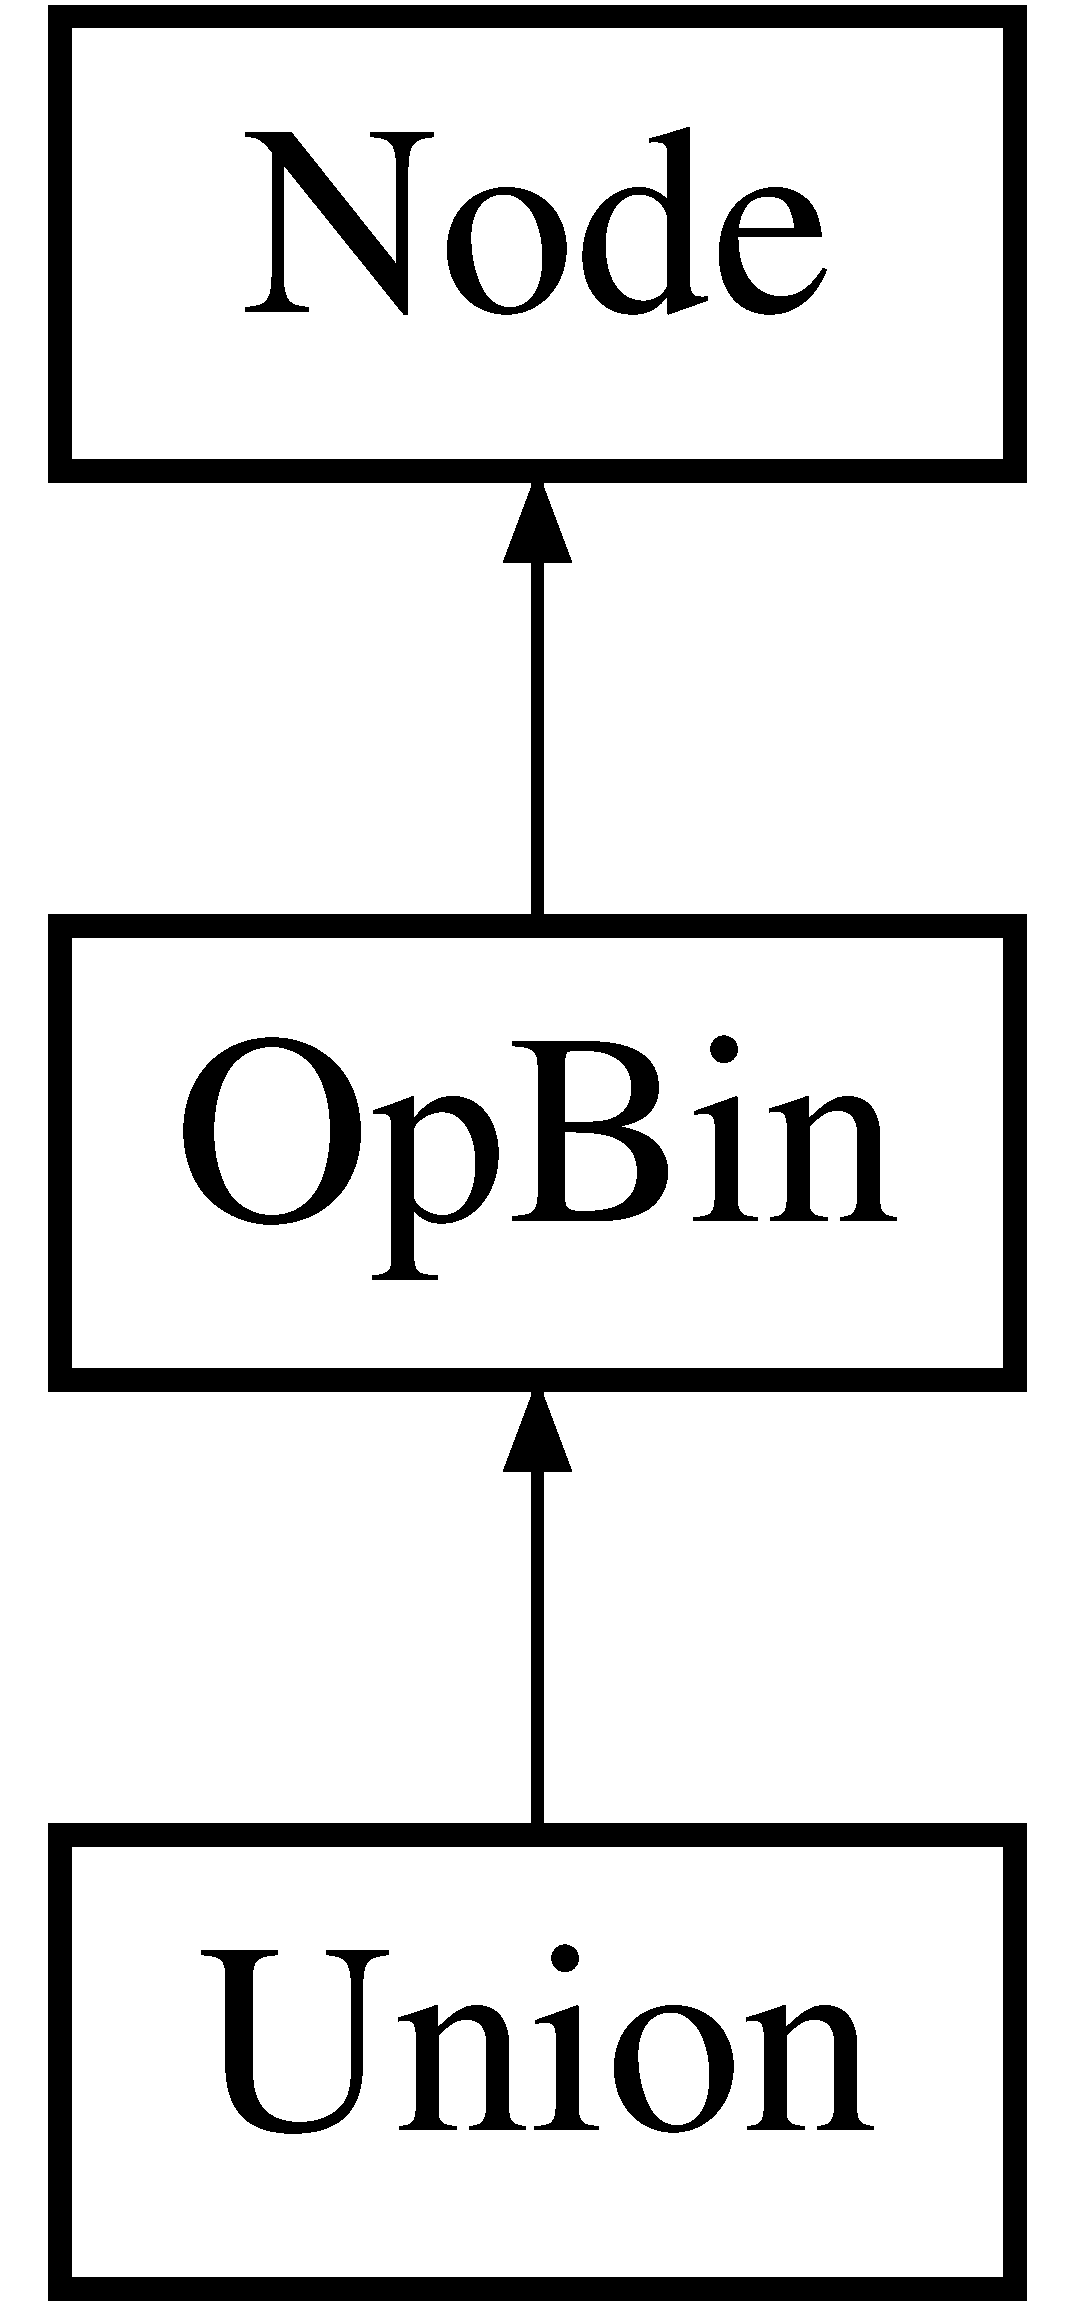
\includegraphics[height=3.000000cm]{class_union}
\end{center}
\end{figure}
\subsection*{\-Public \-Member \-Functions}
\begin{DoxyCompactItemize}
\item 
\hypertarget{class_union_aa5437274642585a29ae3de688d13d854}{
{\bfseries \-Union} (\hyperlink{class_node}{\-Node} $\ast$, \hyperlink{class_node}{\-Node} $\ast$)}
\label{class_union_aa5437274642585a29ae3de688d13d854}

\item 
int \hyperlink{class_union_afa492095314d22df3372b4b1a3efaeca}{\-Intersect} (const \hyperlink{class_ray}{\-Ray} \&, \hyperlink{class_intersection}{\-Intersection} \&)
\begin{DoxyCompactList}\small\item\em \-Intersecting function. \end{DoxyCompactList}\item 
int \hyperlink{class_union_a2ecdc6c70bd44426bc20d88885ec497f}{\-Intersect} (const \hyperlink{class_ray}{\-Ray} \&, \hyperlink{class_intersection}{\-Intersection} \&, \hyperlink{class_intersection}{\-Intersection} \&)
\begin{DoxyCompactList}\small\item\em \-Intersecting function. \end{DoxyCompactList}\item 
int \hyperlink{class_union_ae9430083fcfdc62199b26db6e511d150}{\-P\-M\-C} (const \hyperlink{class_vector}{\-Vector} \&)
\begin{DoxyCompactList}\small\item\em \-Containing function. \end{DoxyCompactList}\item 
\hypertarget{class_union_aa6784389abd98cb2695dd19013b3fd5d}{
\hyperlink{class_vector}{\-Vector} {\bfseries get\-Emission} ()}
\label{class_union_aa6784389abd98cb2695dd19013b3fd5d}

\item 
\hypertarget{class_union_a3960fc7e0d24a0e67fc936d31339c42f}{
\hyperlink{class_vector}{\-Vector} {\bfseries get\-Color} ()}
\label{class_union_a3960fc7e0d24a0e67fc936d31339c42f}

\item 
\hypertarget{class_union_ae42e6df118a33668b35837f58069d269}{
\hyperlink{class_vector}{\-Vector} {\bfseries get\-Position} ()}
\label{class_union_ae42e6df118a33668b35837f58069d269}

\item 
\hypertarget{class_union_ab5d1751fa3af64b7804db79f4e5e3413}{
int {\bfseries get\-Refl} ()}
\label{class_union_ab5d1751fa3af64b7804db79f4e5e3413}

\item 
\hypertarget{class_union_a7ba79196a182f3ed1dfc50607000d1cc}{
double {\bfseries get\-F} ()}
\label{class_union_a7ba79196a182f3ed1dfc50607000d1cc}

\end{DoxyCompactItemize}


\subsection{\-Detailed \-Description}
\hyperlink{class_union}{\-Union} class. 

\hyperlink{class_union}{\-Union} is a binary operand of the \-C\-S\-G 

\subsection{\-Member \-Function \-Documentation}
\hypertarget{class_union_afa492095314d22df3372b4b1a3efaeca}{
\index{\-Union@{\-Union}!\-Intersect@{\-Intersect}}
\index{\-Intersect@{\-Intersect}!Union@{\-Union}}
\subsubsection[{\-Intersect}]{\setlength{\rightskip}{0pt plus 5cm}int \-Union\-::\-Intersect (
\begin{DoxyParamCaption}
\item[{const {\bf \-Ray} \&}]{, }
\item[{{\bf \-Intersection} \&}]{}
\end{DoxyParamCaption}
)\hspace{0.3cm}{\ttfamily  \mbox{[}virtual\mbox{]}}}}
\label{class_union_afa492095314d22df3372b4b1a3efaeca}


\-Intersecting function. 

\-Compute the intersection between a union and a ray


\begin{DoxyParams}{\-Parameters}
{\em ray} & \-: the ray \\
\hline
{\em t} & \-: the intersection \\
\hline
\end{DoxyParams}


\-Implements \hyperlink{class_node_ac0836475b7b0275dffe5ce89547f6852}{\-Node}.

\hypertarget{class_union_a2ecdc6c70bd44426bc20d88885ec497f}{
\index{\-Union@{\-Union}!\-Intersect@{\-Intersect}}
\index{\-Intersect@{\-Intersect}!Union@{\-Union}}
\subsubsection[{\-Intersect}]{\setlength{\rightskip}{0pt plus 5cm}int \-Union\-::\-Intersect (
\begin{DoxyParamCaption}
\item[{const {\bf \-Ray} \&}]{, }
\item[{{\bf \-Intersection} \&}]{, }
\item[{{\bf \-Intersection} \&}]{}
\end{DoxyParamCaption}
)\hspace{0.3cm}{\ttfamily  \mbox{[}virtual\mbox{]}}}}
\label{class_union_a2ecdc6c70bd44426bc20d88885ec497f}


\-Intersecting function. 

\-Compute the intersections between a union and a ray


\begin{DoxyParams}{\-Parameters}
{\em ray} & \-: the ray \\
\hline
{\em t1} & \-: the first intersection \\
\hline
{\em t2} & \-: the second intersection \\
\hline
\end{DoxyParams}


\-Implements \hyperlink{class_node_a8f308647523fba2603248b83149855a5}{\-Node}.

\hypertarget{class_union_ae9430083fcfdc62199b26db6e511d150}{
\index{\-Union@{\-Union}!\-P\-M\-C@{\-P\-M\-C}}
\index{\-P\-M\-C@{\-P\-M\-C}!Union@{\-Union}}
\subsubsection[{\-P\-M\-C}]{\setlength{\rightskip}{0pt plus 5cm}int \-Union\-::\-P\-M\-C (
\begin{DoxyParamCaption}
\item[{const {\bf \-Vector} \&}]{}
\end{DoxyParamCaption}
)\hspace{0.3cm}{\ttfamily  \mbox{[}virtual\mbox{]}}}}
\label{class_union_ae9430083fcfdc62199b26db6e511d150}


\-Containing function. 

\-Checks if a point is inside the instance


\begin{DoxyParams}{\-Parameters}
{\em u} & \-: the point \\
\hline
\end{DoxyParams}


\-Implements \hyperlink{class_node_aeecdf01a88be40840b65eb34cecc7a3c}{\-Node}.



\-The documentation for this class was generated from the following file\-:\begin{DoxyCompactItemize}
\item 
headers/\hyperlink{union_8h}{union.\-h}\end{DoxyCompactItemize}

\hypertarget{class_vector}{
\section{\-Vector \-Class \-Reference}
\label{class_vector}\index{\-Vector@{\-Vector}}
}


\hyperlink{class_vector}{\-Vector} class.  




{\ttfamily \#include $<$vector.\-h$>$}

\subsection*{\-Public \-Member \-Functions}
\begin{DoxyCompactItemize}
\item 
\hypertarget{class_vector_ac37c37579f774e7caca05777438b35e1}{
{\bfseries \-Vector} (const double \&a, const double \&b, const double \&c)}
\label{class_vector_ac37c37579f774e7caca05777438b35e1}

\item 
\hypertarget{class_vector_a660c349db92ad8c2465487b78953f51c}{
double {\bfseries length} ()}
\label{class_vector_a660c349db92ad8c2465487b78953f51c}

\item 
\hypertarget{class_vector_a8cc4aefe1d880f18feac3426ea8d933e}{
double \& {\bfseries operator\mbox{[}$\,$\mbox{]}} (int i)}
\label{class_vector_a8cc4aefe1d880f18feac3426ea8d933e}

\item 
\hypertarget{class_vector_aaf99974616dc176c949a6eb14ab34685}{
const double {\bfseries operator\mbox{[}$\,$\mbox{]}} (int i) const }
\label{class_vector_aaf99974616dc176c949a6eb14ab34685}

\item 
\hypertarget{class_vector_a439f710d3deeb8609b3428d79630c420}{
\hyperlink{class_vector}{\-Vector} {\bfseries \-Scale} (const \hyperlink{class_vector}{\-Vector} \&b) const }
\label{class_vector_a439f710d3deeb8609b3428d79630c420}

\item 
\hypertarget{class_vector_a55aa4644709bc040a90dbff081bb717a}{
\hyperlink{class_vector}{\-Vector} {\bfseries operator+} () const }
\label{class_vector_a55aa4644709bc040a90dbff081bb717a}

\item 
\hypertarget{class_vector_a1c38f8a4f5f6f9438e3ec8233cfaa6b0}{
\hyperlink{class_vector}{\-Vector} {\bfseries operator-\/} () const }
\label{class_vector_a1c38f8a4f5f6f9438e3ec8233cfaa6b0}

\item 
\hypertarget{class_vector_a669208fe9ad795111df6a54683563c6d}{
\hyperlink{class_vector}{\-Vector} \& {\bfseries operator+=} (const \hyperlink{class_vector}{\-Vector} \&)}
\label{class_vector_a669208fe9ad795111df6a54683563c6d}

\item 
\hypertarget{class_vector_abc58d82a7f0ec941d4f4d66012cf5e83}{
\hyperlink{class_vector}{\-Vector} \& {\bfseries operator-\/=} (const \hyperlink{class_vector}{\-Vector} \&)}
\label{class_vector_abc58d82a7f0ec941d4f4d66012cf5e83}

\item 
\hypertarget{class_vector_aa0ffd0237c0ba122b2a56fb84cdf5378}{
\hyperlink{class_vector}{\-Vector} \& {\bfseries operator$\ast$=} (const \hyperlink{class_vector}{\-Vector} \&)}
\label{class_vector_aa0ffd0237c0ba122b2a56fb84cdf5378}

\item 
\hypertarget{class_vector_a7e0eaf65ee4c031c1a2f1868ce715761}{
\hyperlink{class_vector}{\-Vector} \& {\bfseries operator/=} (const \hyperlink{class_vector}{\-Vector} \&)}
\label{class_vector_a7e0eaf65ee4c031c1a2f1868ce715761}

\item 
\hypertarget{class_vector_a5e9a64ca63bfbbd1a49c34fd10507459}{
\hyperlink{class_vector}{\-Vector} \& {\bfseries operator$\ast$=} (double)}
\label{class_vector_a5e9a64ca63bfbbd1a49c34fd10507459}

\item 
\hypertarget{class_vector_a44879c9208fb830aa748fcf654776ebd}{
\hyperlink{class_vector}{\-Vector} \& {\bfseries operator/=} (double)}
\label{class_vector_a44879c9208fb830aa748fcf654776ebd}

\end{DoxyCompactItemize}
\subsection*{\-Public \-Attributes}
\begin{DoxyCompactItemize}
\item 
\hypertarget{class_vector_a133722e00601091cb2075219da5da6e4}{
double {\bfseries x}}
\label{class_vector_a133722e00601091cb2075219da5da6e4}

\item 
\hypertarget{class_vector_a09a21a140718f234eea348d5058cee0b}{
double {\bfseries y}}
\label{class_vector_a09a21a140718f234eea348d5058cee0b}

\item 
\hypertarget{class_vector_a1b604d674485316754b72494f5fcc960}{
double {\bfseries z}}
\label{class_vector_a1b604d674485316754b72494f5fcc960}

\end{DoxyCompactItemize}
\subsection*{\-Friends}
\begin{DoxyCompactItemize}
\item 
\hypertarget{class_vector_af3fdd2b7487c71d4b20a74e30a95891d}{
\hyperlink{class_vector}{\-Vector} {\bfseries operator+} (const \hyperlink{class_vector}{\-Vector} \&, const \hyperlink{class_vector}{\-Vector} \&)}
\label{class_vector_af3fdd2b7487c71d4b20a74e30a95891d}

\item 
\hypertarget{class_vector_ac4505f13a01e5d3312660626ae4ddebb}{
\hyperlink{class_vector}{\-Vector} {\bfseries operator-\/} (const \hyperlink{class_vector}{\-Vector} \&, const \hyperlink{class_vector}{\-Vector} \&)}
\label{class_vector_ac4505f13a01e5d3312660626ae4ddebb}

\item 
\hypertarget{class_vector_af1d37366ff3e48ec9bb37885cdf89f71}{
double {\bfseries operator$\ast$} (const \hyperlink{class_vector}{\-Vector} \&, const \hyperlink{class_vector}{\-Vector} \&)}
\label{class_vector_af1d37366ff3e48ec9bb37885cdf89f71}

\item 
\hypertarget{class_vector_ad5b5658ce9cdb77c1e02c0716b4446c6}{
\hyperlink{class_vector}{\-Vector} {\bfseries operator$\ast$} (const \hyperlink{class_vector}{\-Vector} \&, double)}
\label{class_vector_ad5b5658ce9cdb77c1e02c0716b4446c6}

\item 
\hypertarget{class_vector_af5e2acc16843ab7b90d3c5755125fef4}{
\hyperlink{class_vector}{\-Vector} {\bfseries operator$\ast$} (double, const \hyperlink{class_vector}{\-Vector} \&)}
\label{class_vector_af5e2acc16843ab7b90d3c5755125fef4}

\item 
\hypertarget{class_vector_adc4d2909e834dd600fae663f2c98a432}{
\hyperlink{class_vector}{\-Vector} {\bfseries operator/} (const \hyperlink{class_vector}{\-Vector} \&, double)}
\label{class_vector_adc4d2909e834dd600fae663f2c98a432}

\item 
\hypertarget{class_vector_a7ac2d5db6d0258692a3278bf90069c6a}{
\hyperlink{class_vector}{\-Vector} {\bfseries operator/} (const \hyperlink{class_vector}{\-Vector} \&, const \hyperlink{class_vector}{\-Vector} \&)}
\label{class_vector_a7ac2d5db6d0258692a3278bf90069c6a}

\item 
\hypertarget{class_vector_aca63309fd635cd4fa72e5335b76e1c21}{
int {\bfseries operator==} (const \hyperlink{class_vector}{\-Vector} \&, const \hyperlink{class_vector}{\-Vector} \&)}
\label{class_vector_aca63309fd635cd4fa72e5335b76e1c21}

\item 
\hypertarget{class_vector_ade583d2f018e2ff120d78c0e0998a422}{
int {\bfseries operator!=} (const \hyperlink{class_vector}{\-Vector} \&, const \hyperlink{class_vector}{\-Vector} \&)}
\label{class_vector_ade583d2f018e2ff120d78c0e0998a422}

\item 
\hypertarget{class_vector_ac6abefa6e71400fc5de5ca68b5ca7651}{
int {\bfseries operator$<$} (const \hyperlink{class_vector}{\-Vector} \&, const \hyperlink{class_vector}{\-Vector} \&)}
\label{class_vector_ac6abefa6e71400fc5de5ca68b5ca7651}

\item 
\hypertarget{class_vector_ac4e29ac8916987f0d304c44c6a98afed}{
int {\bfseries operator$>$} (const \hyperlink{class_vector}{\-Vector} \&, const \hyperlink{class_vector}{\-Vector} \&)}
\label{class_vector_ac4e29ac8916987f0d304c44c6a98afed}

\item 
\hypertarget{class_vector_a42522fc19a307d9ceca3ec122e81fea7}{
\hyperlink{class_vector}{\-Vector} \hyperlink{class_vector_a42522fc19a307d9ceca3ec122e81fea7}{min} (const \hyperlink{class_vector}{\-Vector} \&, const \hyperlink{class_vector}{\-Vector} \&)}
\label{class_vector_a42522fc19a307d9ceca3ec122e81fea7}

\begin{DoxyCompactList}\small\item\em \-Return a new vector with coordinates set to the minimum coordinates of the two argument vectors. \end{DoxyCompactList}\item 
\hypertarget{class_vector_ac7fa5b7201c15daca80958d11a93c79a}{
\hyperlink{class_vector}{\-Vector} \hyperlink{class_vector_ac7fa5b7201c15daca80958d11a93c79a}{max} (const \hyperlink{class_vector}{\-Vector} \&, const \hyperlink{class_vector}{\-Vector} \&)}
\label{class_vector_ac7fa5b7201c15daca80958d11a93c79a}

\begin{DoxyCompactList}\small\item\em \-Return a new vector with coordinates set to the maximum coordinates of the two argument vectors. \end{DoxyCompactList}\item 
\hypertarget{class_vector_ac32c66eb175b3fc3a00aa2b972af9a72}{
\hyperlink{class_vector}{\-Vector} \hyperlink{class_vector_ac32c66eb175b3fc3a00aa2b972af9a72}{\-Orthogonal} (const \hyperlink{class_vector}{\-Vector} \&)}
\label{class_vector_ac32c66eb175b3fc3a00aa2b972af9a72}

\begin{DoxyCompactList}\small\item\em \-Returns a new vector orthogonal to the argument vector. \end{DoxyCompactList}\item 
\hypertarget{class_vector_aafee6c0f5a420bd4f869b62d099222b3}{
double \hyperlink{class_vector_aafee6c0f5a420bd4f869b62d099222b3}{\-Norm} (const \hyperlink{class_vector}{\-Vector} \&)}
\label{class_vector_aafee6c0f5a420bd4f869b62d099222b3}

\begin{DoxyCompactList}\small\item\em \-Compute the \-Euclidean norm of a vector. \end{DoxyCompactList}\item 
\hypertarget{class_vector_a49c314e89f483ee7c68fca2baf9920b1}{
\hyperlink{class_vector}{\-Vector} \hyperlink{class_vector_a49c314e89f483ee7c68fca2baf9920b1}{\-Normalized} (const \hyperlink{class_vector}{\-Vector} \&)}
\label{class_vector_a49c314e89f483ee7c68fca2baf9920b1}

\begin{DoxyCompactList}\small\item\em \-Compute the \-Euclidean norm of a vector. \end{DoxyCompactList}\end{DoxyCompactItemize}


\subsection{\-Detailed \-Description}
\hyperlink{class_vector}{\-Vector} class. 

\hyperlink{class_vector}{\-Vector} is a data structure 

\-The documentation for this class was generated from the following file\-:\begin{DoxyCompactItemize}
\item 
headers/\hyperlink{vector_8h}{vector.\-h}\end{DoxyCompactItemize}

\chapter{\-File \-Documentation}
\hypertarget{box_8h}{
\section{headers/box.h \-File \-Reference}
\label{box_8h}\index{headers/box.\-h@{headers/box.\-h}}
}


class \hyperlink{class_box}{\-Box} header  


{\ttfamily \#include \char`\"{}primitive.\-h\char`\"{}}\*
\subsection*{\-Classes}
\begin{DoxyCompactItemize}
\item 
class \hyperlink{class_box}{\-Box}
\begin{DoxyCompactList}\small\item\em \hyperlink{class_box}{\-Box} class. \end{DoxyCompactList}\end{DoxyCompactItemize}


\subsection{\-Detailed \-Description}
class \hyperlink{class_box}{\-Box} header \begin{DoxyAuthor}{\-Author}
\-Gimenez \-Tom, \-Roumier \-Vincent, \-Matéo \-Camille 
\end{DoxyAuthor}
\begin{DoxyVersion}{\-Version}
1.\-0 
\end{DoxyVersion}
\begin{DoxyDate}{\-Date}
01 octobre 2011
\end{DoxyDate}
\-Containing \hyperlink{class_box}{\-Box} class 
\hypertarget{cylinder_8h}{
\section{headers/cylinder.h \-File \-Reference}
\label{cylinder_8h}\index{headers/cylinder.\-h@{headers/cylinder.\-h}}
}


class \hyperlink{class_cylinder}{\-Cylinder} header  


{\ttfamily \#include \char`\"{}primitive.\-h\char`\"{}}\*
\subsection*{\-Classes}
\begin{DoxyCompactItemize}
\item 
class \hyperlink{class_cylinder}{\-Cylinder}
\begin{DoxyCompactList}\small\item\em \hyperlink{class_cylinder}{\-Cylinder} class. \end{DoxyCompactList}\end{DoxyCompactItemize}


\subsection{\-Detailed \-Description}
class \hyperlink{class_cylinder}{\-Cylinder} header \begin{DoxyAuthor}{\-Author}
\-Gimenez \-Tom, \-Roumier \-Vincent, \-Matéo \-Camille 
\end{DoxyAuthor}
\begin{DoxyVersion}{\-Version}
1.\-0 
\end{DoxyVersion}
\begin{DoxyDate}{\-Date}
01 octobre 2011
\end{DoxyDate}
\-Containing \hyperlink{class_cylinder}{\-Cylinder} class 
\hypertarget{diff_8h}{
\section{headers/diff.h \-File \-Reference}
\label{diff_8h}\index{headers/diff.\-h@{headers/diff.\-h}}
}


class \hyperlink{class_diff}{\-Diff} header  


{\ttfamily \#include \char`\"{}opbin.\-h\char`\"{}}\*
\subsection*{\-Classes}
\begin{DoxyCompactItemize}
\item 
class \hyperlink{class_diff}{\-Diff}
\begin{DoxyCompactList}\small\item\em \hyperlink{class_diff}{\-Diff} class. \end{DoxyCompactList}\end{DoxyCompactItemize}


\subsection{\-Detailed \-Description}
class \hyperlink{class_diff}{\-Diff} header \begin{DoxyAuthor}{\-Author}
\-Gimenez \-Tom, \-Roumier \-Vincent, \-Matéo \-Camille 
\end{DoxyAuthor}
\begin{DoxyVersion}{\-Version}
1.\-0 
\end{DoxyVersion}
\begin{DoxyDate}{\-Date}
01 octobre 2011
\end{DoxyDate}
\-Containing \hyperlink{class_diff}{\-Diff} class 
\hypertarget{inter_8h}{
\section{headers/inter.h \-File \-Reference}
\label{inter_8h}\index{headers/inter.\-h@{headers/inter.\-h}}
}


class \hyperlink{class_inter}{\-Inter} header  


{\ttfamily \#include \char`\"{}opbin.\-h\char`\"{}}\*
\subsection*{\-Classes}
\begin{DoxyCompactItemize}
\item 
class \hyperlink{class_inter}{\-Inter}
\begin{DoxyCompactList}\small\item\em \hyperlink{class_inter}{\-Inter} class. \end{DoxyCompactList}\end{DoxyCompactItemize}


\subsection{\-Detailed \-Description}
class \hyperlink{class_inter}{\-Inter} header \begin{DoxyAuthor}{\-Author}
\-Gimenez \-Tom, \-Roumier \-Vincent, \-Matéo \-Camille 
\end{DoxyAuthor}
\begin{DoxyVersion}{\-Version}
1.\-0 
\end{DoxyVersion}
\begin{DoxyDate}{\-Date}
01 octobre 2011
\end{DoxyDate}
\-Containing inter class 
\hypertarget{intersection_8h}{
\section{headers/intersection.h \-File \-Reference}
\label{intersection_8h}\index{headers/intersection.\-h@{headers/intersection.\-h}}
}


class \hyperlink{class_intersection}{\-Intersection} header  


{\ttfamily \#include \char`\"{}vector.\-h\char`\"{}}\*
\subsection*{\-Classes}
\begin{DoxyCompactItemize}
\item 
class \hyperlink{class_intersection}{\-Intersection}
\begin{DoxyCompactList}\small\item\em \hyperlink{class_intersection}{\-Intersection} class. \end{DoxyCompactList}\end{DoxyCompactItemize}


\subsection{\-Detailed \-Description}
class \hyperlink{class_intersection}{\-Intersection} header \begin{DoxyAuthor}{\-Author}
\-Gimenez \-Tom, \-Roumier \-Vincent, \-Mat�o \-Camille 
\end{DoxyAuthor}
\begin{DoxyVersion}{\-Version}
1.\-0 
\end{DoxyVersion}
\begin{DoxyDate}{\-Date}
01 octobre 2011
\end{DoxyDate}
\-Containing \hyperlink{class_intersection}{\-Intersection} class 
\hypertarget{_matrix4_d_8h}{
\section{headers/\-Matrix4\-D.h \-File \-Reference}
\label{_matrix4_d_8h}\index{headers/\-Matrix4\-D.\-h@{headers/\-Matrix4\-D.\-h}}
}


class \hyperlink{class_matrix4_df}{\-Matrix4\-Df} header  


{\ttfamily \#include $<$stdio.\-h$>$}\*
{\ttfamily \#include \char`\"{}vector.\-h\char`\"{}}\*
\subsection*{\-Classes}
\begin{DoxyCompactItemize}
\item 
class \hyperlink{class_matrix4_df}{\-Matrix4\-Df}
\begin{DoxyCompactList}\small\item\em \-Matri4\-Df class. \end{DoxyCompactList}\end{DoxyCompactItemize}
\subsection*{\-Functions}
\begin{DoxyCompactItemize}
\item 
\hypertarget{_matrix4_d_8h_aa8b49e6b5d204995a97bdcdff56e1ff8}{
\hyperlink{class_matrix4_df}{\-Matrix4\-Df} {\bfseries operator+} (const \hyperlink{class_matrix4_df}{\-Matrix4\-Df} \&m1, const \hyperlink{class_matrix4_df}{\-Matrix4\-Df} \&m2)}
\label{_matrix4_d_8h_aa8b49e6b5d204995a97bdcdff56e1ff8}

\item 
\hypertarget{_matrix4_d_8h_a4cd11065198b040b1bc3e3026835b368}{
\hyperlink{class_matrix4_df}{\-Matrix4\-Df} {\bfseries operator-\/} (const \hyperlink{class_matrix4_df}{\-Matrix4\-Df} \&m1, const \hyperlink{class_matrix4_df}{\-Matrix4\-Df} \&m2)}
\label{_matrix4_d_8h_a4cd11065198b040b1bc3e3026835b368}

\item 
\hypertarget{_matrix4_d_8h_ac4aad75706ee141200622ba4c5b59aae}{
\hyperlink{class_matrix4_df}{\-Matrix4\-Df} {\bfseries operator$\ast$} (const \hyperlink{class_matrix4_df}{\-Matrix4\-Df} \&m1, const \hyperlink{class_matrix4_df}{\-Matrix4\-Df} \&m2)}
\label{_matrix4_d_8h_ac4aad75706ee141200622ba4c5b59aae}

\item 
\hypertarget{_matrix4_d_8h_a6e845817f2128ac90102744e21e98a27}{
\hyperlink{class_matrix4_df}{\-Matrix4\-Df} {\bfseries operator-\/} (const \hyperlink{class_matrix4_df}{\-Matrix4\-Df} \&m)}
\label{_matrix4_d_8h_a6e845817f2128ac90102744e21e98a27}

\item 
\hypertarget{_matrix4_d_8h_a58ee3262b5ce3fba49f1a3de3cac112e}{
\hyperlink{class_matrix4_df}{\-Matrix4\-Df} {\bfseries operator$\ast$} (const float f, const \hyperlink{class_matrix4_df}{\-Matrix4\-Df} \&m)}
\label{_matrix4_d_8h_a58ee3262b5ce3fba49f1a3de3cac112e}

\item 
\hypertarget{_matrix4_d_8h_aa310e684369ce51992642e9371f87228}{
\hyperlink{class_matrix4_df}{\-Matrix4\-Df} {\bfseries operator$\ast$} (const \hyperlink{class_matrix4_df}{\-Matrix4\-Df} \&m, const float f)}
\label{_matrix4_d_8h_aa310e684369ce51992642e9371f87228}

\end{DoxyCompactItemize}


\subsection{\-Detailed \-Description}
class \hyperlink{class_matrix4_df}{\-Matrix4\-Df} header \begin{DoxyAuthor}{\-Author}
\-Gimenez \-Tom, \-Roumier \-Vincent, \-Mat�o \-Camille 
\end{DoxyAuthor}
\begin{DoxyVersion}{\-Version}
1.\-0 
\end{DoxyVersion}
\begin{DoxyDate}{\-Date}
01 octobre 2011
\end{DoxyDate}
\-Containing \hyperlink{class_matrix4_df}{\-Matrix4\-Df} class 
\hypertarget{node_8h}{
\section{headers/node.h \-File \-Reference}
\label{node_8h}\index{headers/node.\-h@{headers/node.\-h}}
}


class \hyperlink{class_node}{\-Node} header  


{\ttfamily \#include \char`\"{}vector.\-h\char`\"{}}\*
{\ttfamily \#include \char`\"{}ray.\-h\char`\"{}}\*
{\ttfamily \#include \char`\"{}intersection.\-h\char`\"{}}\*
\subsection*{\-Classes}
\begin{DoxyCompactItemize}
\item 
class \hyperlink{class_node}{\-Node}
\begin{DoxyCompactList}\small\item\em \hyperlink{class_node}{\-Node} class. \end{DoxyCompactList}\end{DoxyCompactItemize}


\subsection{\-Detailed \-Description}
class \hyperlink{class_node}{\-Node} header \begin{DoxyAuthor}{\-Author}
\-Gimenez \-Tom, \-Roumier \-Vincent, \-Matéo \-Camille 
\end{DoxyAuthor}
\begin{DoxyVersion}{\-Version}
1.\-0 
\end{DoxyVersion}
\begin{DoxyDate}{\-Date}
01 octobre 2011
\end{DoxyDate}
\-Containing \hyperlink{class_node}{\-Node} class 
\hypertarget{opbin_8h}{
\section{headers/opbin.h \-File \-Reference}
\label{opbin_8h}\index{headers/opbin.\-h@{headers/opbin.\-h}}
}


class \hyperlink{class_op_bin}{\-Op\-Bin} header  


{\ttfamily \#include \char`\"{}node.\-h\char`\"{}}\*
\subsection*{\-Classes}
\begin{DoxyCompactItemize}
\item 
class \hyperlink{class_op_bin}{\-Op\-Bin}
\begin{DoxyCompactList}\small\item\em \hyperlink{class_op_bin}{\-Op\-Bin} class. \end{DoxyCompactList}\end{DoxyCompactItemize}


\subsection{\-Detailed \-Description}
class \hyperlink{class_op_bin}{\-Op\-Bin} header \begin{DoxyAuthor}{\-Author}
\-Gimenez \-Tom, \-Roumier \-Vincent, \-Matéo \-Camille 
\end{DoxyAuthor}
\begin{DoxyVersion}{\-Version}
1.\-0 
\end{DoxyVersion}
\begin{DoxyDate}{\-Date}
01 octobre 2011
\end{DoxyDate}
\-Containing \hyperlink{class_op_bin}{\-Op\-Bin} class 
\hypertarget{primitive_8h}{
\section{headers/primitive.h \-File \-Reference}
\label{primitive_8h}\index{headers/primitive.\-h@{headers/primitive.\-h}}
}


class \hyperlink{class_primitive}{\-Primitive} header  


{\ttfamily \#include \char`\"{}node.\-h\char`\"{}}\*
\subsection*{\-Classes}
\begin{DoxyCompactItemize}
\item 
class \hyperlink{class_primitive}{\-Primitive}
\begin{DoxyCompactList}\small\item\em \hyperlink{class_primitive}{\-Primitive} class. \end{DoxyCompactList}\end{DoxyCompactItemize}


\subsection{\-Detailed \-Description}
class \hyperlink{class_primitive}{\-Primitive} header \begin{DoxyAuthor}{\-Author}
\-Gimenez \-Tom, \-Roumier \-Vincent, \-Matéo \-Camille 
\end{DoxyAuthor}
\begin{DoxyVersion}{\-Version}
1.\-0 
\end{DoxyVersion}
\begin{DoxyDate}{\-Date}
01 octobre 2011
\end{DoxyDate}
\-Containing \hyperlink{class_primitive}{\-Primitive} class 
\hypertarget{ray_8h}{
\section{headers/ray.h \-File \-Reference}
\label{ray_8h}\index{headers/ray.\-h@{headers/ray.\-h}}
}


class \hyperlink{class_ray}{\-Ray} header  


{\ttfamily \#include \char`\"{}vector.\-h\char`\"{}}\*
\subsection*{\-Classes}
\begin{DoxyCompactItemize}
\item 
class \hyperlink{class_ray}{\-Ray}
\begin{DoxyCompactList}\small\item\em \hyperlink{class_ray}{\-Ray} class. \end{DoxyCompactList}\end{DoxyCompactItemize}


\subsection{\-Detailed \-Description}
class \hyperlink{class_ray}{\-Ray} header \begin{DoxyAuthor}{\-Author}
\-Gimenez \-Tom, \-Roumier \-Vincent, \-Matéo \-Camille 
\end{DoxyAuthor}
\begin{DoxyVersion}{\-Version}
1.\-0 
\end{DoxyVersion}
\begin{DoxyDate}{\-Date}
01 octobre 2011
\end{DoxyDate}
\-Containing the ray class 
\hypertarget{rotation_8h}{
\section{headers/rotation.h \-File \-Reference}
\label{rotation_8h}\index{headers/rotation.\-h@{headers/rotation.\-h}}
}


class \hyperlink{class_rotation}{\-Rotation} header  


{\ttfamily \#include \char`\"{}transfo.\-h\char`\"{}}\*
\subsection*{\-Classes}
\begin{DoxyCompactItemize}
\item 
class \hyperlink{class_rotation}{\-Rotation}
\begin{DoxyCompactList}\small\item\em \hyperlink{class_rotation}{\-Rotation} class. \end{DoxyCompactList}\end{DoxyCompactItemize}


\subsection{\-Detailed \-Description}
class \hyperlink{class_rotation}{\-Rotation} header \begin{DoxyAuthor}{\-Author}
\-Gimenez \-Tom, \-Roumier \-Vincent, \-Matéo \-Camille 
\end{DoxyAuthor}
\begin{DoxyVersion}{\-Version}
1.\-0 
\end{DoxyVersion}
\begin{DoxyDate}{\-Date}
01 octobre 2011
\end{DoxyDate}
\-Containing \hyperlink{class_rotation}{\-Rotation} class 
\hypertarget{sphere_8h}{
\section{headers/sphere.h \-File \-Reference}
\label{sphere_8h}\index{headers/sphere.\-h@{headers/sphere.\-h}}
}


class \hyperlink{class_sphere}{\-Sphere} header  


{\ttfamily \#include \char`\"{}primitive.\-h\char`\"{}}\*
\subsection*{\-Classes}
\begin{DoxyCompactItemize}
\item 
class \hyperlink{class_sphere}{\-Sphere}
\begin{DoxyCompactList}\small\item\em \hyperlink{class_sphere}{\-Sphere} class. \end{DoxyCompactList}\end{DoxyCompactItemize}


\subsection{\-Detailed \-Description}
class \hyperlink{class_sphere}{\-Sphere} header \begin{DoxyAuthor}{\-Author}
\-Gimenez \-Tom, \-Roumier \-Vincent, \-Matéo \-Camille 
\end{DoxyAuthor}
\begin{DoxyVersion}{\-Version}
1.\-0 
\end{DoxyVersion}
\begin{DoxyDate}{\-Date}
01 octobre 2011
\end{DoxyDate}
\-Containing \hyperlink{class_sphere}{\-Sphere} class 
\hypertarget{transfo_8h}{
\section{headers/transfo.h \-File \-Reference}
\label{transfo_8h}\index{headers/transfo.\-h@{headers/transfo.\-h}}
}


class \hyperlink{class_transfo}{\-Transfo} header  


{\ttfamily \#include \char`\"{}node.\-h\char`\"{}}\*
{\ttfamily \#include \char`\"{}\-Matrix4\-D.\-h\char`\"{}}\*
\subsection*{\-Classes}
\begin{DoxyCompactItemize}
\item 
class \hyperlink{class_transfo}{\-Transfo}
\begin{DoxyCompactList}\small\item\em \hyperlink{class_transfo}{\-Transfo} class. \end{DoxyCompactList}\end{DoxyCompactItemize}


\subsection{\-Detailed \-Description}
class \hyperlink{class_transfo}{\-Transfo} header \begin{DoxyAuthor}{\-Author}
\-Gimenez \-Tom, \-Roumier \-Vincent, \-Matéo \-Camille 
\end{DoxyAuthor}
\begin{DoxyVersion}{\-Version}
1.\-0 
\end{DoxyVersion}
\begin{DoxyDate}{\-Date}
01 octobre 2011
\end{DoxyDate}
\-Containing \hyperlink{class_transfo}{\-Transfo} class 
\hypertarget{translation_8h}{
\section{headers/translation.h \-File \-Reference}
\label{translation_8h}\index{headers/translation.\-h@{headers/translation.\-h}}
}


class \hyperlink{class_translation}{\-Translation} header  


{\ttfamily \#include \char`\"{}transfo.\-h\char`\"{}}\*
\subsection*{\-Classes}
\begin{DoxyCompactItemize}
\item 
class \hyperlink{class_translation}{\-Translation}
\begin{DoxyCompactList}\small\item\em \hyperlink{class_translation}{\-Translation} class. \end{DoxyCompactList}\end{DoxyCompactItemize}


\subsection{\-Detailed \-Description}
class \hyperlink{class_translation}{\-Translation} header \begin{DoxyAuthor}{\-Author}
\-Gimenez \-Tom, \-Roumier \-Vincent, \-Matéo \-Camille 
\end{DoxyAuthor}
\begin{DoxyVersion}{\-Version}
1.\-0 
\end{DoxyVersion}
\begin{DoxyDate}{\-Date}
01 octobre 2011
\end{DoxyDate}
\-Containing \hyperlink{class_translation}{\-Translation} class 
\hypertarget{triangle_8h}{
\section{headers/triangle.h \-File \-Reference}
\label{triangle_8h}\index{headers/triangle.\-h@{headers/triangle.\-h}}
}


class \hyperlink{class_triangle}{\-Triangle} header  


{\ttfamily \#include \char`\"{}primitive.\-h\char`\"{}}\*
\subsection*{\-Classes}
\begin{DoxyCompactItemize}
\item 
class \hyperlink{class_triangle}{\-Triangle}
\begin{DoxyCompactList}\small\item\em \hyperlink{class_triangle}{\-Triangle} class. \end{DoxyCompactList}\end{DoxyCompactItemize}


\subsection{\-Detailed \-Description}
class \hyperlink{class_triangle}{\-Triangle} header \begin{DoxyAuthor}{\-Author}
\-Gimenez \-Tom, \-Roumier \-Vincent, \-Matéo \-Camille 
\end{DoxyAuthor}
\begin{DoxyVersion}{\-Version}
1.\-0 
\end{DoxyVersion}
\begin{DoxyDate}{\-Date}
01 octobre 2011
\end{DoxyDate}
\-Containing \hyperlink{class_triangle}{\-Triangle} class 
\hypertarget{union_8h}{
\section{headers/union.h \-File \-Reference}
\label{union_8h}\index{headers/union.\-h@{headers/union.\-h}}
}


class \hyperlink{class_union}{\-Union} header  


{\ttfamily \#include \char`\"{}opbin.\-h\char`\"{}}\*
\subsection*{\-Classes}
\begin{DoxyCompactItemize}
\item 
class \hyperlink{class_union}{\-Union}
\begin{DoxyCompactList}\small\item\em \hyperlink{class_union}{\-Union} class. \end{DoxyCompactList}\end{DoxyCompactItemize}


\subsection{\-Detailed \-Description}
class \hyperlink{class_union}{\-Union} header \begin{DoxyAuthor}{\-Author}
\-Gimenez \-Tom, \-Roumier \-Vincent, \-Matéo \-Camille 
\end{DoxyAuthor}
\begin{DoxyVersion}{\-Version}
1.\-0 
\end{DoxyVersion}
\begin{DoxyDate}{\-Date}
01 octobre 2011
\end{DoxyDate}
\-Containing \hyperlink{class_union}{\-Union} class 
\hypertarget{vector_8h}{
\section{headers/vector.h \-File \-Reference}
\label{vector_8h}\index{headers/vector.\-h@{headers/vector.\-h}}
}


class \hyperlink{class_vector}{\-Vector} header  


{\ttfamily \#include $<$math.\-h$>$}\*
\subsection*{\-Classes}
\begin{DoxyCompactItemize}
\item 
class \hyperlink{class_vector}{\-Vector}
\begin{DoxyCompactList}\small\item\em \hyperlink{class_vector}{\-Vector} class. \end{DoxyCompactList}\end{DoxyCompactItemize}
\subsection*{\-Functions}
\begin{DoxyCompactItemize}
\item 
\hypertarget{vector_8h_ac5f0a089acb6275fac236e00ac42789d}{
double {\bfseries min} (const double \&a, const double \&b)}
\label{vector_8h_ac5f0a089acb6275fac236e00ac42789d}

\item 
\hypertarget{vector_8h_ac7fdd2194c30e5ffe8102f6022f26347}{
double {\bfseries max} (const double \&a, const double \&b)}
\label{vector_8h_ac7fdd2194c30e5ffe8102f6022f26347}

\item 
\hypertarget{vector_8h_a9c00c752511686e3db8ba0c53583f0e0}{
\hyperlink{class_vector}{\-Vector} {\bfseries operator+} (const \hyperlink{class_vector}{\-Vector} \&u, const \hyperlink{class_vector}{\-Vector} \&v)}
\label{vector_8h_a9c00c752511686e3db8ba0c53583f0e0}

\item 
\hypertarget{vector_8h_add405a753e522f16540553c852e69e8b}{
\hyperlink{class_vector}{\-Vector} {\bfseries operator-\/} (const \hyperlink{class_vector}{\-Vector} \&u, const \hyperlink{class_vector}{\-Vector} \&v)}
\label{vector_8h_add405a753e522f16540553c852e69e8b}

\item 
\hypertarget{vector_8h_a27386e77e8c4567d36d0808d17a42153}{
double {\bfseries operator$\ast$} (const \hyperlink{class_vector}{\-Vector} \&u, const \hyperlink{class_vector}{\-Vector} \&v)}
\label{vector_8h_a27386e77e8c4567d36d0808d17a42153}

\item 
\hypertarget{vector_8h_a7a141ef07b1e73bb59583280e7df7a8b}{
\hyperlink{class_vector}{\-Vector} {\bfseries operator$\ast$} (const \hyperlink{class_vector}{\-Vector} \&u, double a)}
\label{vector_8h_a7a141ef07b1e73bb59583280e7df7a8b}

\item 
\hypertarget{vector_8h_aba1ce8114d5b0da5206927a26dca4e50}{
\hyperlink{class_vector}{\-Vector} {\bfseries operator$\ast$} (double a, const \hyperlink{class_vector}{\-Vector} \&v)}
\label{vector_8h_aba1ce8114d5b0da5206927a26dca4e50}

\item 
\hypertarget{vector_8h_acadb130279e2be4d38e143c23e01a310}{
\hyperlink{class_vector}{\-Vector} {\bfseries operator/} (const \hyperlink{class_vector}{\-Vector} \&u, const \hyperlink{class_vector}{\-Vector} \&v)}
\label{vector_8h_acadb130279e2be4d38e143c23e01a310}

\item 
\hypertarget{vector_8h_adda2172f93f7cf451d766e35c6451905}{
\hyperlink{class_vector}{\-Vector} {\bfseries operator/} (const \hyperlink{class_vector}{\-Vector} \&u, double a)}
\label{vector_8h_adda2172f93f7cf451d766e35c6451905}

\item 
\hypertarget{vector_8h_a0b0f847fcfa336ae1c2f2b044f98defa}{
int {\bfseries operator==} (const \hyperlink{class_vector}{\-Vector} \&u, const \hyperlink{class_vector}{\-Vector} \&v)}
\label{vector_8h_a0b0f847fcfa336ae1c2f2b044f98defa}

\item 
\hypertarget{vector_8h_a7426b0f487baf38b42d6e528be1fea87}{
int {\bfseries operator!=} (const \hyperlink{class_vector}{\-Vector} \&u, const \hyperlink{class_vector}{\-Vector} \&v)}
\label{vector_8h_a7426b0f487baf38b42d6e528be1fea87}

\item 
\hypertarget{vector_8h_af90b4e3482e18ba87ba91dac37f85813}{
double \hyperlink{vector_8h_af90b4e3482e18ba87ba91dac37f85813}{\-Norm} (const \hyperlink{class_vector}{\-Vector} \&u)}
\label{vector_8h_af90b4e3482e18ba87ba91dac37f85813}

\begin{DoxyCompactList}\small\item\em \-Compute the \-Euclidean norm of a vector. \end{DoxyCompactList}\item 
\hypertarget{vector_8h_a69dac1e81907adf00b7ac711610542a6}{
\hyperlink{class_vector}{\-Vector} \hyperlink{vector_8h_a69dac1e81907adf00b7ac711610542a6}{\-Normalized} (const \hyperlink{class_vector}{\-Vector} \&u)}
\label{vector_8h_a69dac1e81907adf00b7ac711610542a6}

\begin{DoxyCompactList}\small\item\em \-Compute the \-Euclidean norm of a vector. \end{DoxyCompactList}\item 
\hypertarget{vector_8h_a0a2f9eba6ff48b8f598a64232ef683c1}{
int {\bfseries operator$<$} (const \hyperlink{class_vector}{\-Vector} \&a, const \hyperlink{class_vector}{\-Vector} \&b)}
\label{vector_8h_a0a2f9eba6ff48b8f598a64232ef683c1}

\item 
\hypertarget{vector_8h_a88a303557e59cc8767f097ece0d7e171}{
int {\bfseries operator$>$} (const \hyperlink{class_vector}{\-Vector} \&a, const \hyperlink{class_vector}{\-Vector} \&b)}
\label{vector_8h_a88a303557e59cc8767f097ece0d7e171}

\item 
\hypertarget{vector_8h_abfd5ae418eb7fae08f5f208c22764d9e}{
\hyperlink{class_vector}{\-Vector} \hyperlink{vector_8h_abfd5ae418eb7fae08f5f208c22764d9e}{min} (const \hyperlink{class_vector}{\-Vector} \&a, const \hyperlink{class_vector}{\-Vector} \&b)}
\label{vector_8h_abfd5ae418eb7fae08f5f208c22764d9e}

\begin{DoxyCompactList}\small\item\em \-Return a new vector with coordinates set to the minimum coordinates of the two argument vectors. \end{DoxyCompactList}\item 
\hypertarget{vector_8h_afb93cfbea29400cb7e64af1c14e9e79e}{
\hyperlink{class_vector}{\-Vector} \hyperlink{vector_8h_afb93cfbea29400cb7e64af1c14e9e79e}{max} (const \hyperlink{class_vector}{\-Vector} \&a, const \hyperlink{class_vector}{\-Vector} \&b)}
\label{vector_8h_afb93cfbea29400cb7e64af1c14e9e79e}

\begin{DoxyCompactList}\small\item\em \-Return a new vector with coordinates set to the maximum coordinates of the two argument vectors. \end{DoxyCompactList}\item 
\hypertarget{vector_8h_ab377ffb2508b52674542487885f7b4f1}{
\hyperlink{class_vector}{\-Vector} \hyperlink{vector_8h_ab377ffb2508b52674542487885f7b4f1}{\-Orthogonal} (const \hyperlink{class_vector}{\-Vector} \&u)}
\label{vector_8h_ab377ffb2508b52674542487885f7b4f1}

\begin{DoxyCompactList}\small\item\em \-Returns a new vector orthogonal to the argument vector. \end{DoxyCompactList}\end{DoxyCompactItemize}


\subsection{\-Detailed \-Description}
class \hyperlink{class_vector}{\-Vector} header \begin{DoxyAuthor}{\-Author}
\-Gimenez \-Tom, \-Roumier \-Vincent, \-Mat�o \-Camille 
\end{DoxyAuthor}
\begin{DoxyVersion}{\-Version}
1.\-0 
\end{DoxyVersion}
\begin{DoxyDate}{\-Date}
01 octobre 2011
\end{DoxyDate}
\-Containing \hyperlink{class_vector}{\-Vector} class 
\printindex
\end{document}
